\chapter{Instalação do \LaTeX}
\label{cap:instalacao}

Caso tenha optado por instalar o \LaTeX\ em seu computador, você precisa seguir as instruções dessa seção. Note que, por questões históricas, o \LaTeX é diferente da maioria dos programas Windows. O \LaTeX\ foi criado em 1983 e é baseado no \TeX\ que foi criado em 1978, enquanto o Windows 95 só foi lançado em 1995. Dessa forma o LaTeX é muito anterior a definição dos padrões que os programas Windows seguem atualmente. A principal consequência disso é que o \LaTeX não possui uma interface gráfica. Dessa forma, para usarmos o \LaTeX no Windows, precisamos instalar dois programas:

\begin{itemize}
    \item o MiKTeX que fornece o LaTeX propriamente dito e
\item uma interface gráfica para usá-lo.
\end{itemize}

Por comodidade podemos também instalar um programa para gerenciar a bibliografia. A seguir explicamos passo a passo como instalar cada um desses programas.

Existem diversas interfaces gráficas para o \LaTeX\ disponíveis, cada um pode usar a que preferir uma vez que essa escolha não influencia no resultado gerado. O único cuidado é escolher uma interface que realmente use o \LaTeX\ e não alguma das suas variações. Caso alguém tenha curiosidade, essa página da Wikipédia lista os editores para \LaTeX mais comuns: \url{https://en.wikipedia.org/wiki/Comparison\_of\_TeX\_editors}.

Qualquer editor que edite o código (\textit{source}) e tenha suporte para unicode (utf8) pode ser usado. Aqui mostro como instalar o TeXmaker, pois ele é gratuito, é multiplataforma e tem disponíveis as funcionalidades mais importantes.

\section{Instalando o MiKTeX}

MikTeX é o pacote que contem o \LaTeX\ e vários outros programas auxiliares necessários. Como o conjunto completo de todas as funcionalidades do \LaTeX\ é grande, o site oferece duas opções de instalação, a básica e a completa. A seguir mostramos passo a passo as duas formas de instalar o MikTeX.

A instalação completa é demorada e ocupa mais espaço em disco, pois precisa baixar muitos arquivos, mas fornece todas as funcionalidades do \LaTeX, sem restrições. A instalação básica é mais simples e rápida, mas vamos precisar instalar posteriormente alguns pacotes extras necessários. Cada um pode escolher a forma que preferir, mas prestem muita atenção aos detalhes.

No momento em que esse documento foi escrito a versão mais atualizada do MiKTeX era a versão 20.11. Quando for instalar sempre escolha a última versão disponível.

\subsection{Instalação Básica do MikTeX}

A instalação básica do MikTeX é inicialmente mais simples, porém no futuro será necessário instalar cada pacote faltante quando for necessário utilizá-los.

\begin{enumerate}
\item Entre na página de downloads do MiKTeX: \url{http://miktex.org/download};
\item Clique em download para baixar o arquivo de instalação;
\begin{figure}[!ht]
  \centering
  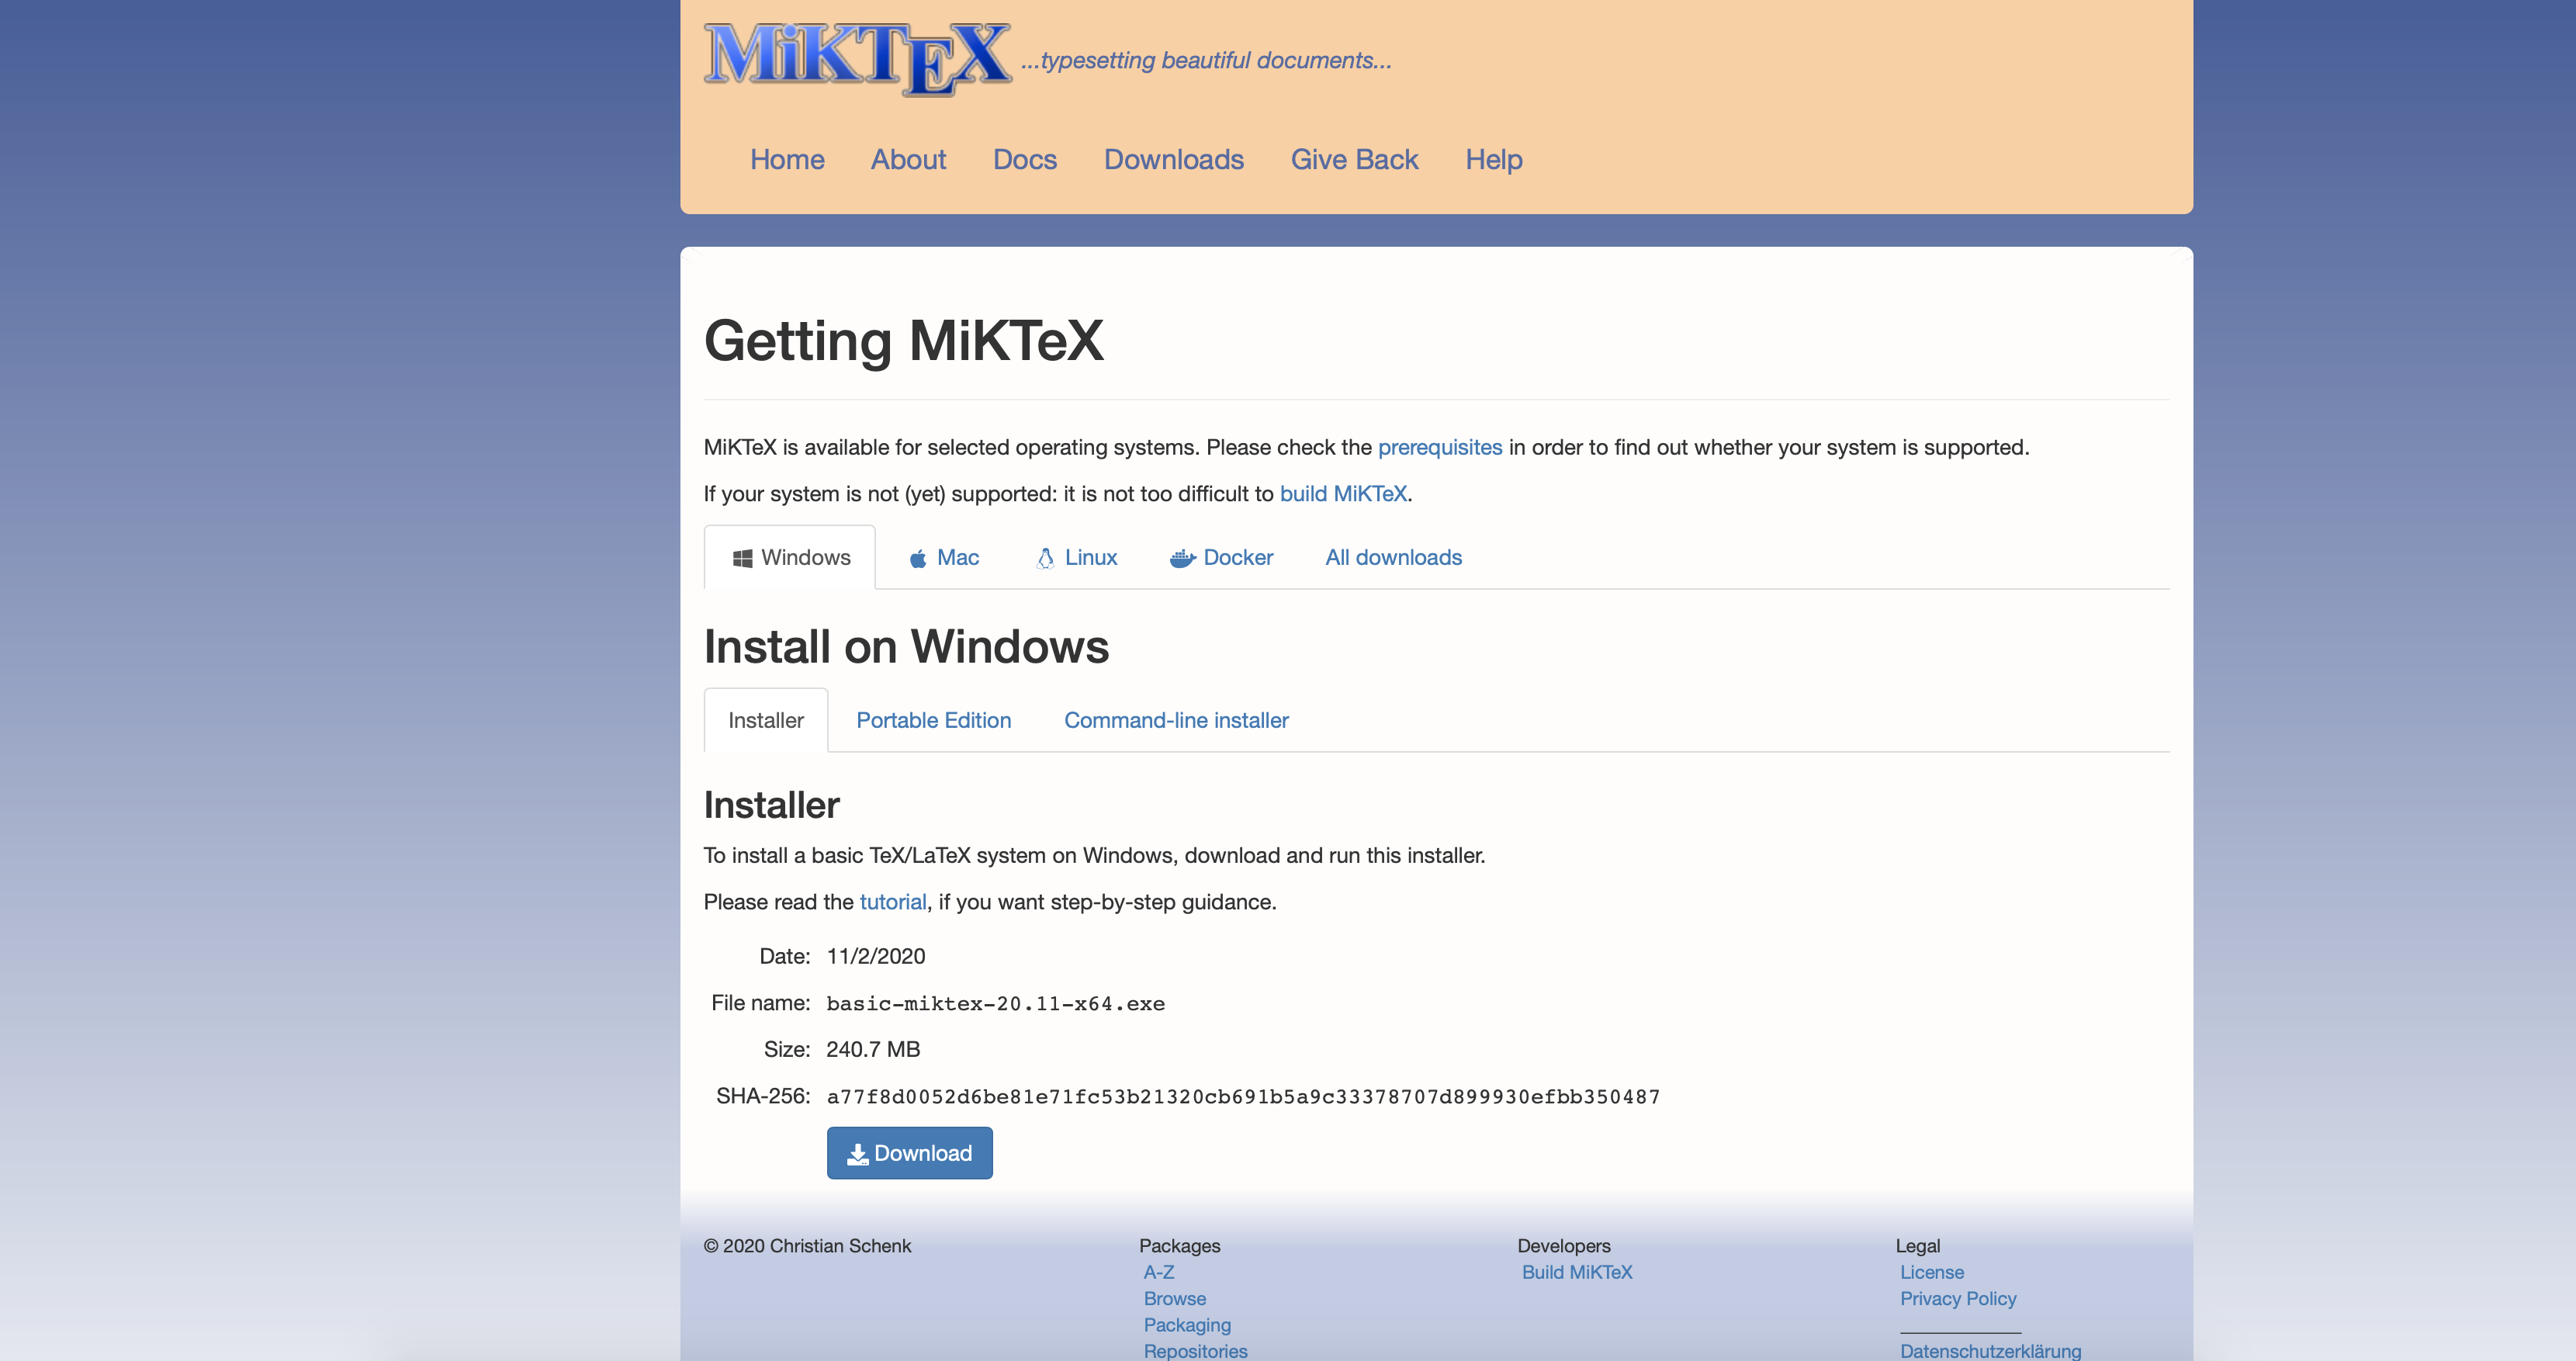
\includegraphics[width=1.0\textwidth]{./fig/miktex01}
  \caption{Site para download do MikTex}
  \label{fig:miktex01}
  \fontefig{Elaborada pelo autor}
\end{figure}
\item Rode o programa baixado;
\item Aceite os termos da \textit{copying conditions};
\begin{figure}[H]
  \centering
  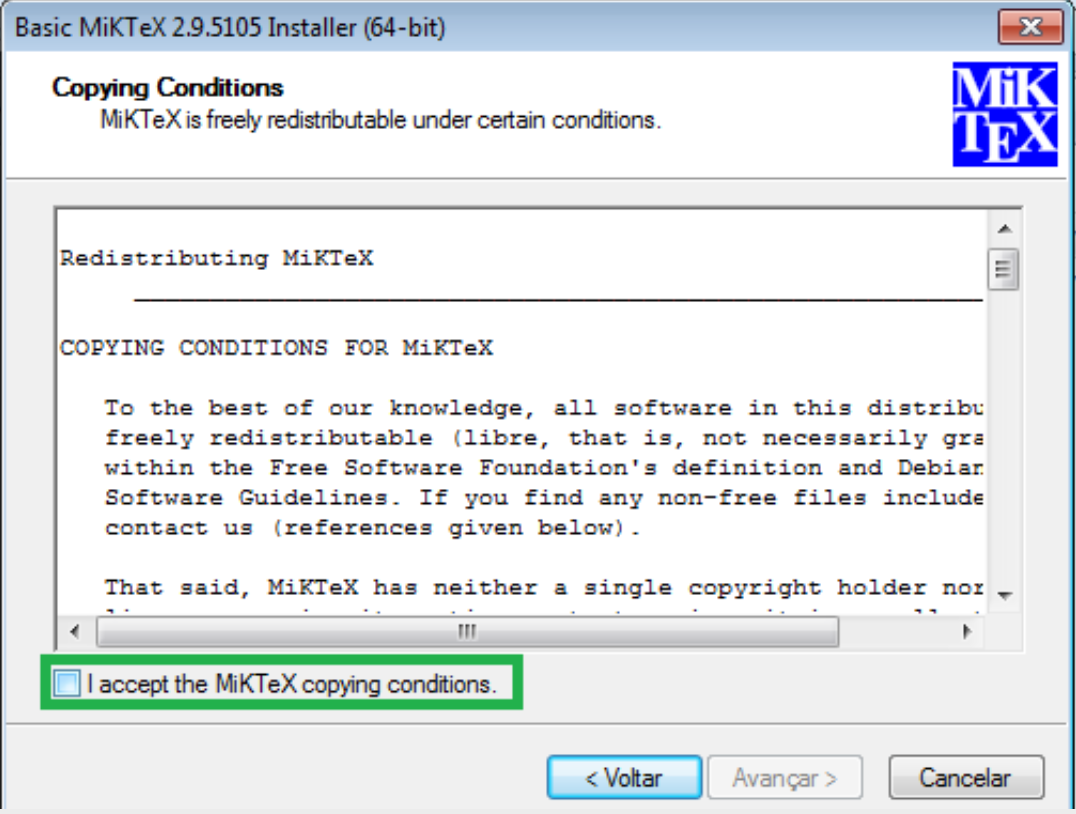
\includegraphics[width=0.6\textwidth]{./fig/miktex02}
  \caption{Instalação do MikTex - Aceitação dos termos.}
  \fontefig{Elaborada pelo autor.}
\end{figure}
\item Selecione instalar para todos os usuários do sistema;
\begin{figure}[H]
  \centering
  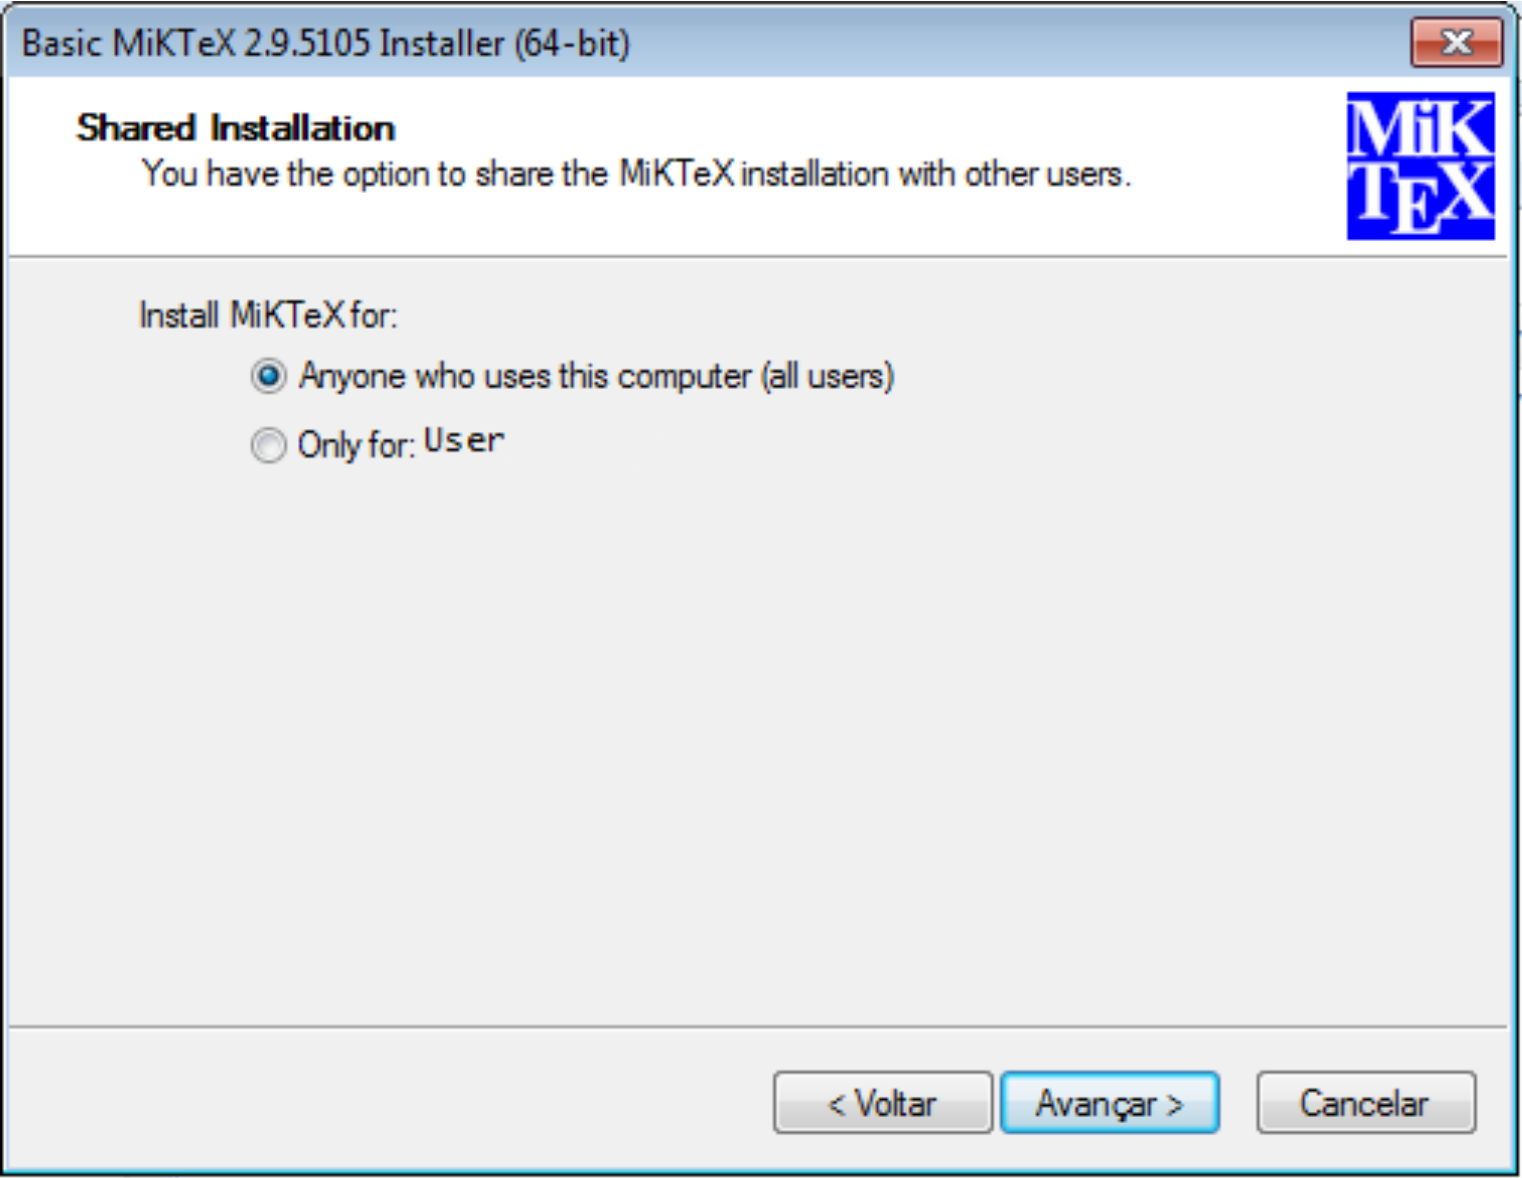
\includegraphics[width=0.6\textwidth]{./fig/miktex03}
  \caption{Instalação do MikTex - Seleção de usuários.}
  \fontefig{Elaborada pelo autor.}
\end{figure}
\item Escolha onde instalar o MiKTeX. É recomendado manter o local sugerido;
\begin{figure}[H]
  \centering
  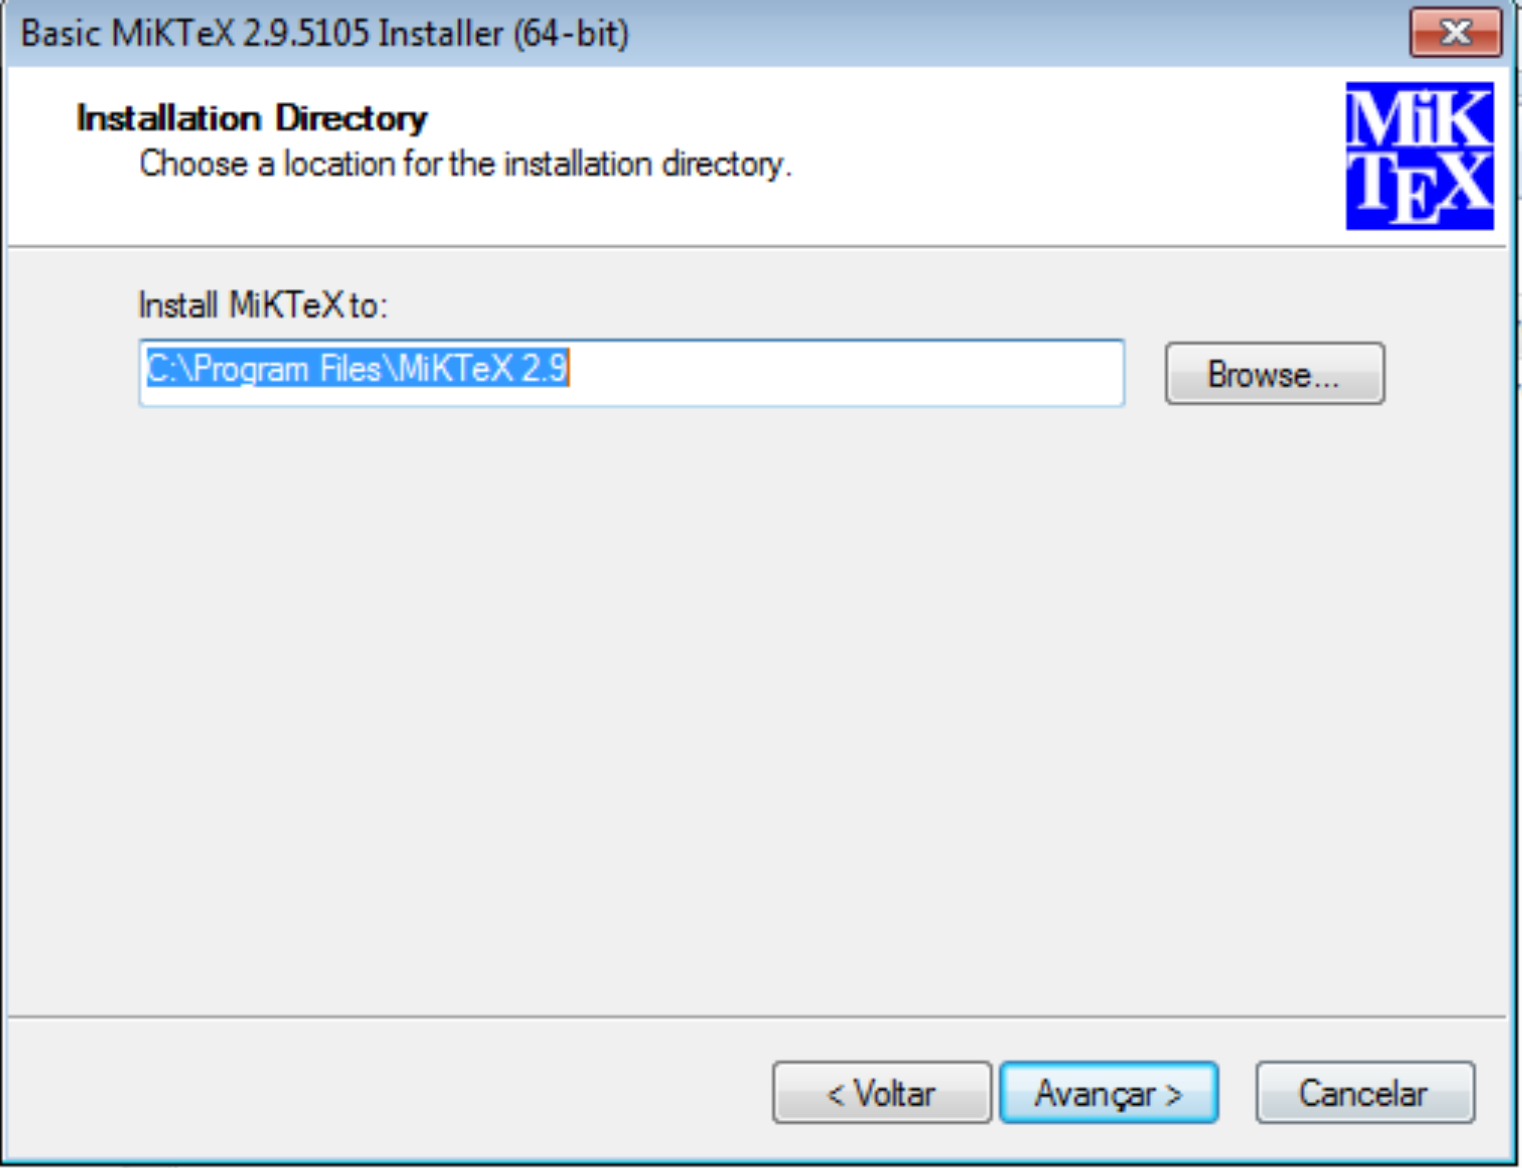
\includegraphics[width=0.6\textwidth]{./fig/miktex04}
  \caption{Instalação do MikTex - Local de instalação.}
  \fontefig{Elaborada pelo autor.}
\end{figure}
\item Escolha as opções solicitadas, é recomendado manter as sugestões A4 para o tipo de papel e \textbf{Ask me First} para instalar os pacotes faltantes;
\begin{figure}[H]
  \centering
  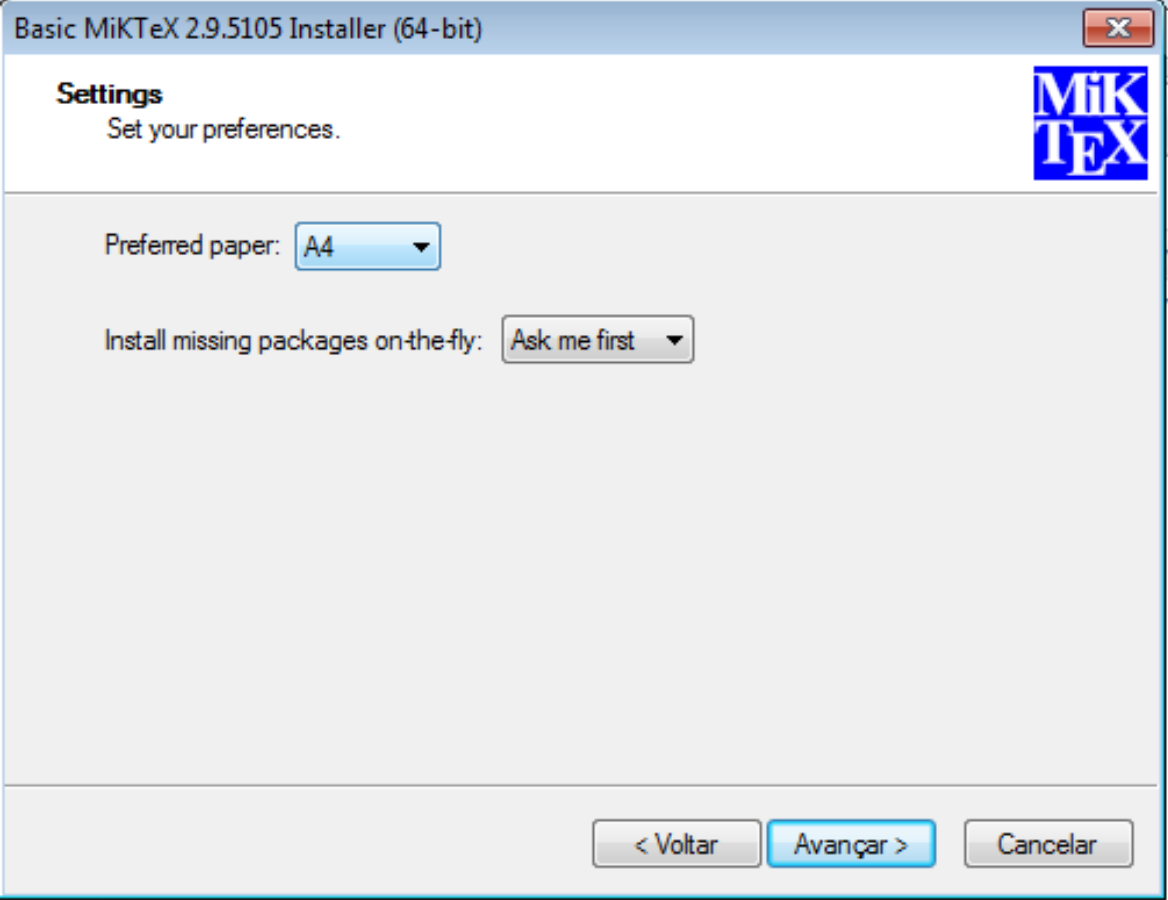
\includegraphics[width=0.6\textwidth]{./fig/miktex05}
  \caption{Instalação do MikTex - Seleção de opções.}
  \fontefig{Elaborada pelo autor.}
\end{figure}
\item Clique em \textbf{Start} para iniciar a instalação;
\begin{figure}[H]
  \centering
  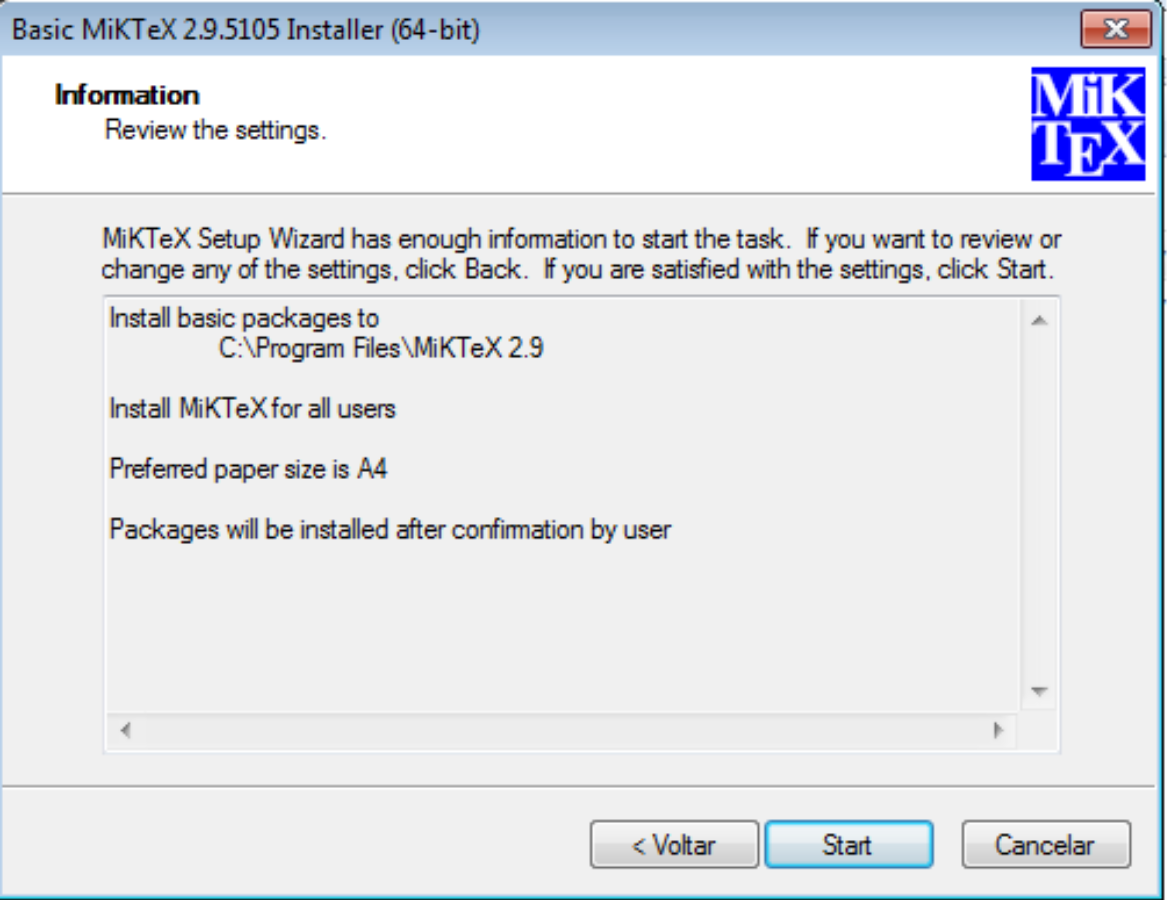
\includegraphics[width=0.6\textwidth]{./fig/miktex06}
  \caption{Instalação do MikTex - Início da instalação.}
  \fontefig{Elaborada pelo autor.}
\end{figure}
\item Autorize que o programa faça alterações no sistema;
\item Aguarde o final da instalação;
\begin{figure}[H]
  \centering
  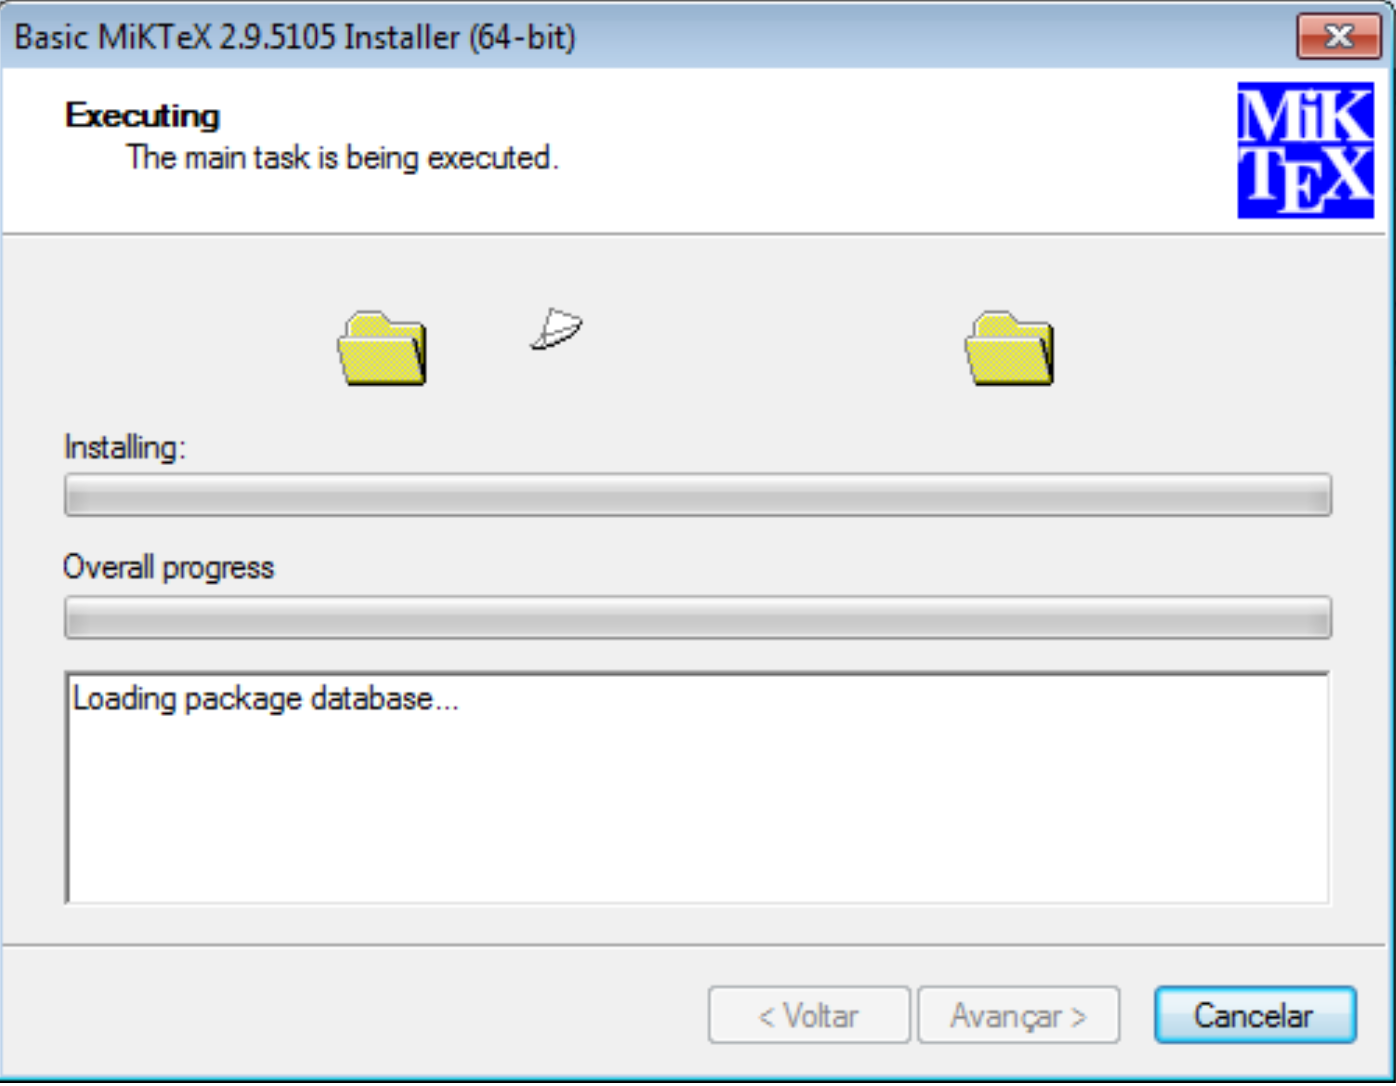
\includegraphics[width=0.6\textwidth]{./fig/miktex07}
  \caption{Instalação do MikTex - Execução da instalação.}
  \fontefig{Elaborada pelo autor.}
\end{figure}
\item Permita que o MikTeX busque por atualizações na internet;
\item Se desejar, desabilite a opção \textbf{Tell me more};
\item Conclua a instalação clicando em \textbf{Close}.
\begin{figure}[H]
  \centering
  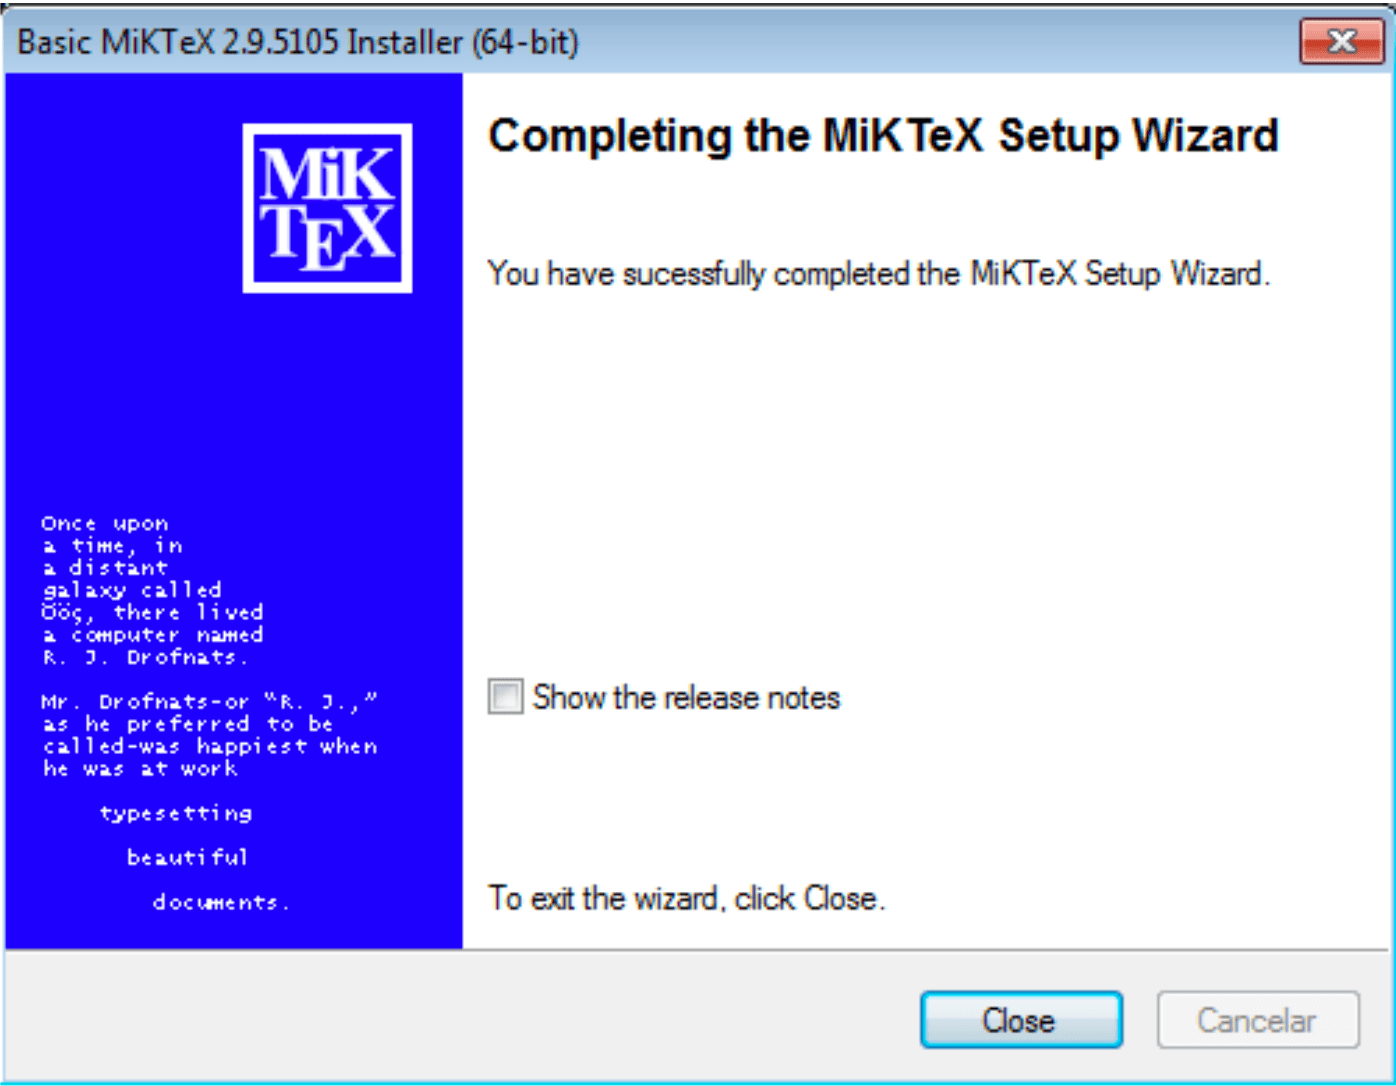
\includegraphics[width=0.6\textwidth]{./fig/miktex08}
  \caption{Instalação do MikTex - Fim da instalação.}
  \fontefig{Elaborada pelo autor.}
\end{figure}
\end{enumerate}

\subsection{Instalação Completa do MikTeX}

\textbf{ATENÇÃO:} A versão completa do MiKTeX é chamada Net \textbf{Installer} e não está na página inicial de download da página do MikTeX.

O processo de instalação da versão básica é simples, sendo exatamente igual ao processo de instalação de qualquer outro programa. Já a versão completa, é necessário abrir o instalador duas vezes. A primeira tem o objetivo de baixar e escolher uma pasta para armazenar os arquivos necessários. Uma vez baixado todos os arquivos, é necessário abrir o instalador novamente e indicar a pasta onde os arquivos foram baixados. Em seguida, o MikTeX será instalado.
 
O passo a passo para a instalação do MikTeX completo pode ser visto a seguir \cite{miktexfull}.

\begin{enumerate}
\item Entre na página de downloads do MiKTeX: \url{http://miktex.org/download} (\autoref{fig:miktex01});
\item \textbf{NÃO} clique no botão de download;
\item Selecione a aba \textbf{All Downloads};
\begin{figure}[H]
  \centering
  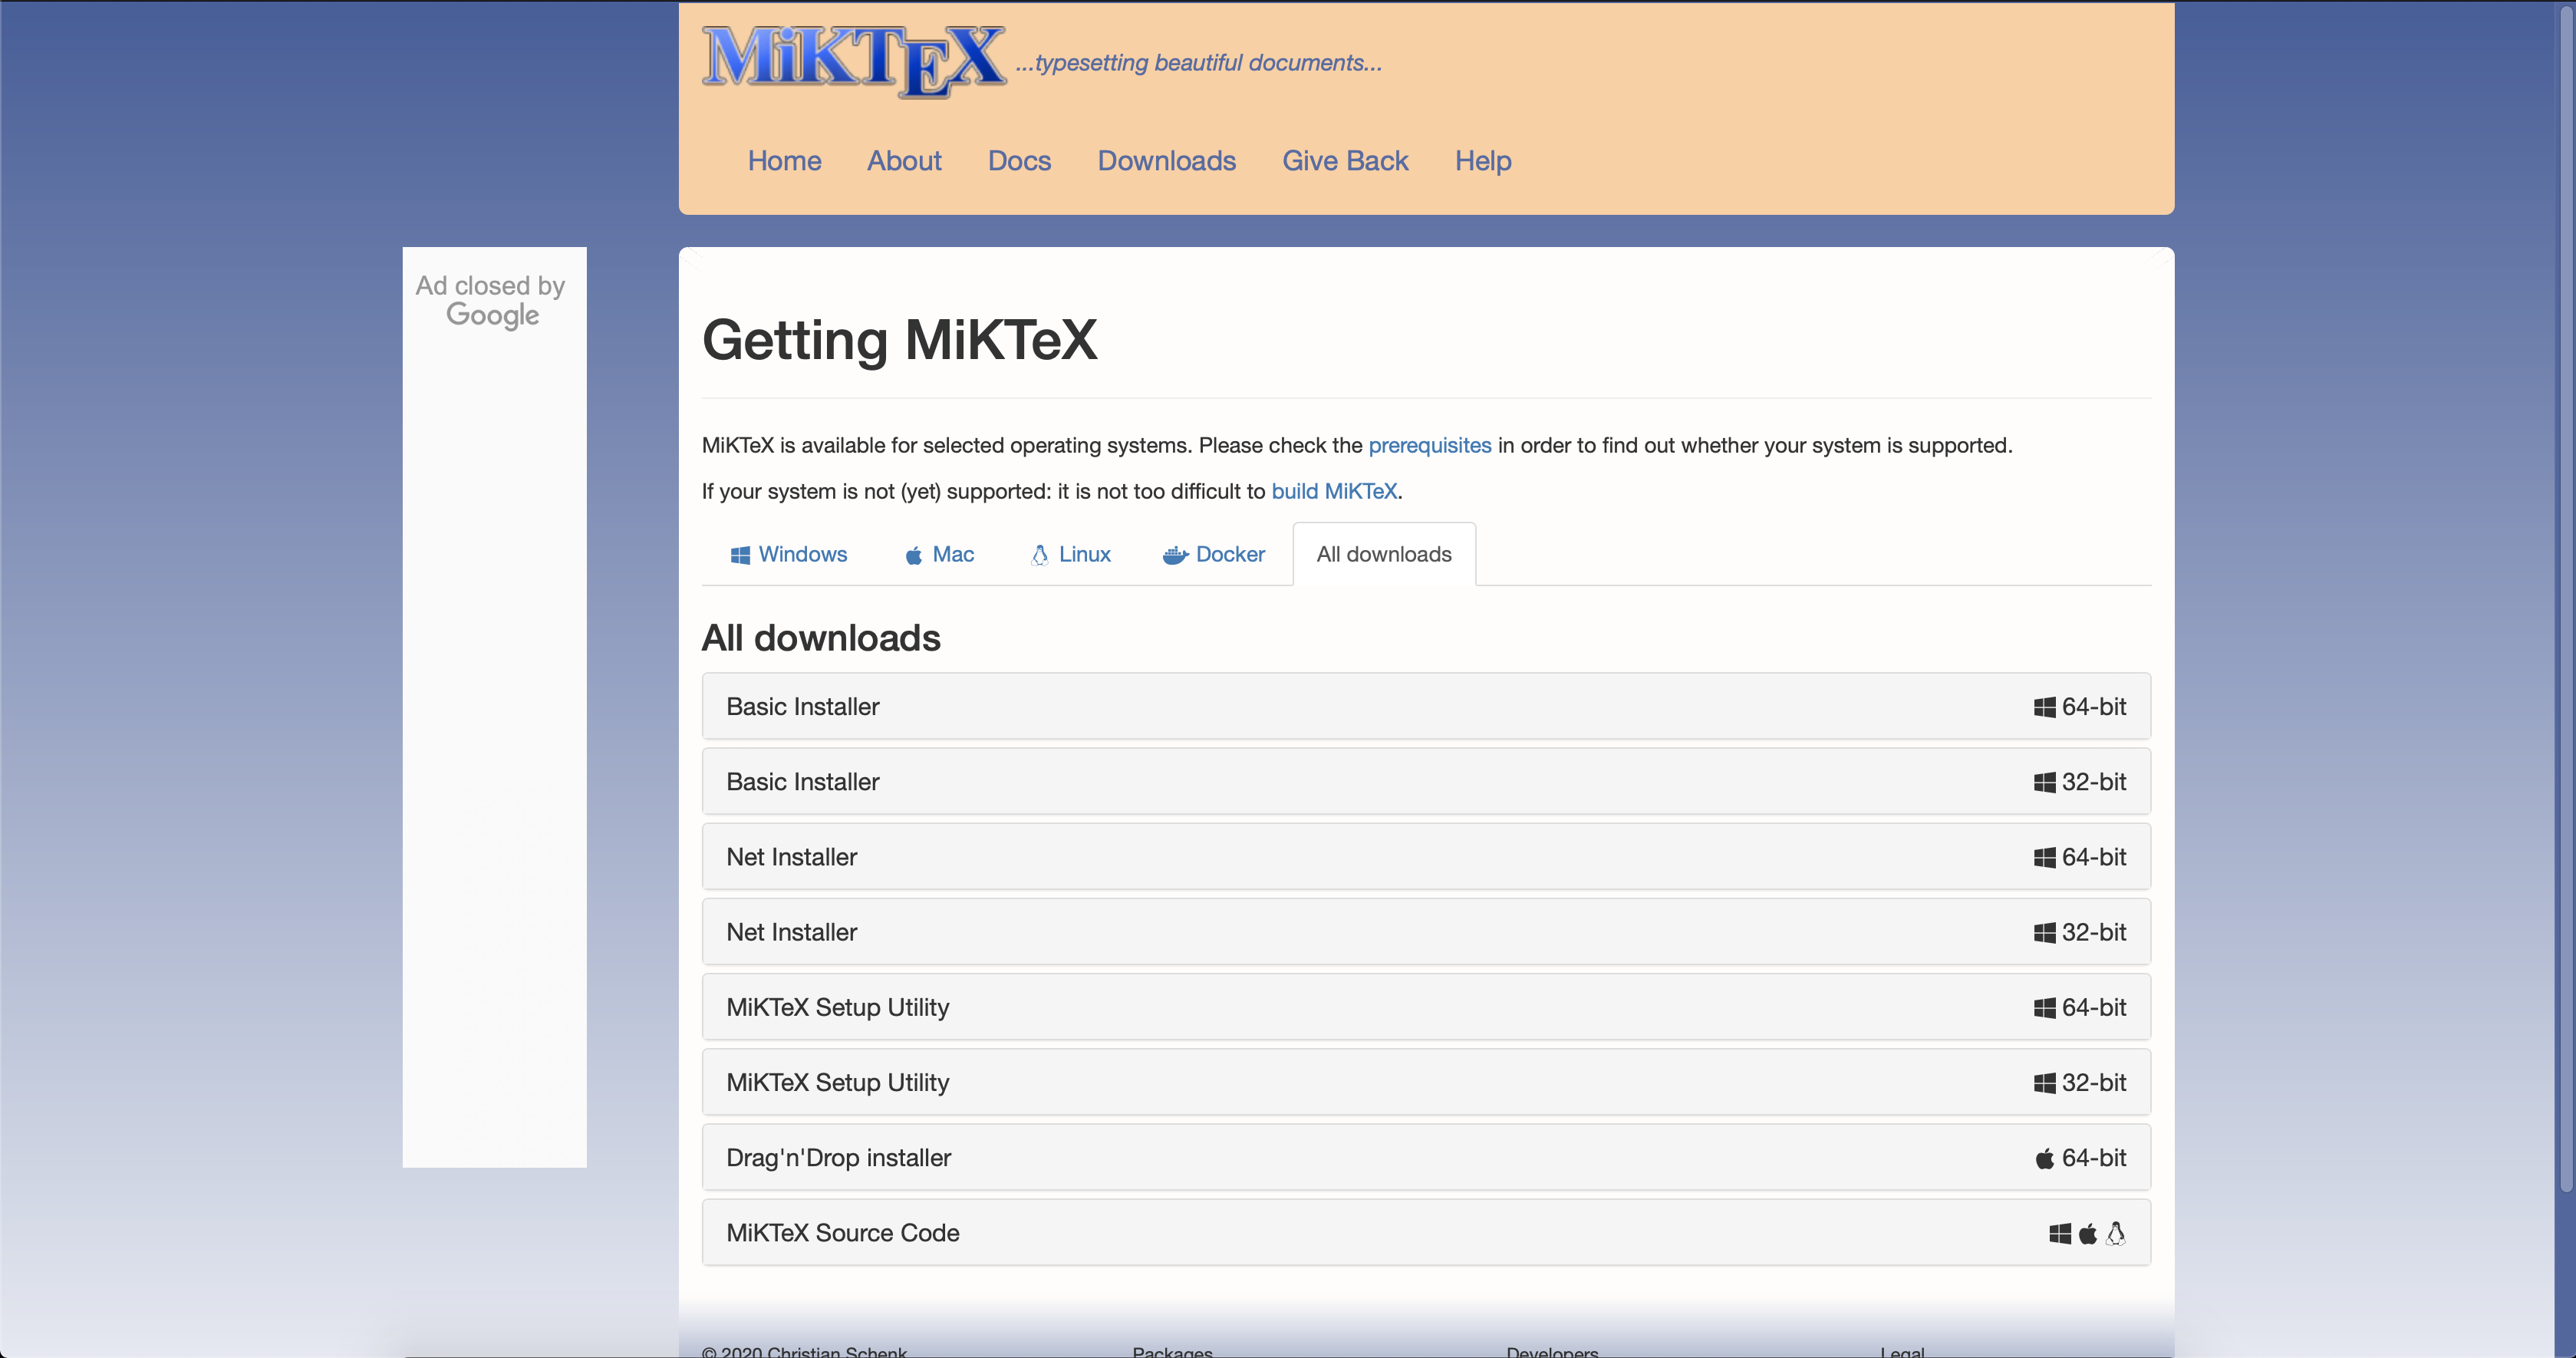
\includegraphics[width=1.0\textwidth]{./fig/miktex09}
  \caption{Instalação completa do MikTex - Página com todos os downloads.}
  \fontefig{Elaborada pelo autor}
\end{figure}
\item Selecione a opção \textbf{Net Installer}, escolha 32 ou 64 bits de acordo com seu computador;
\begin{figure}[H]
  \centering
  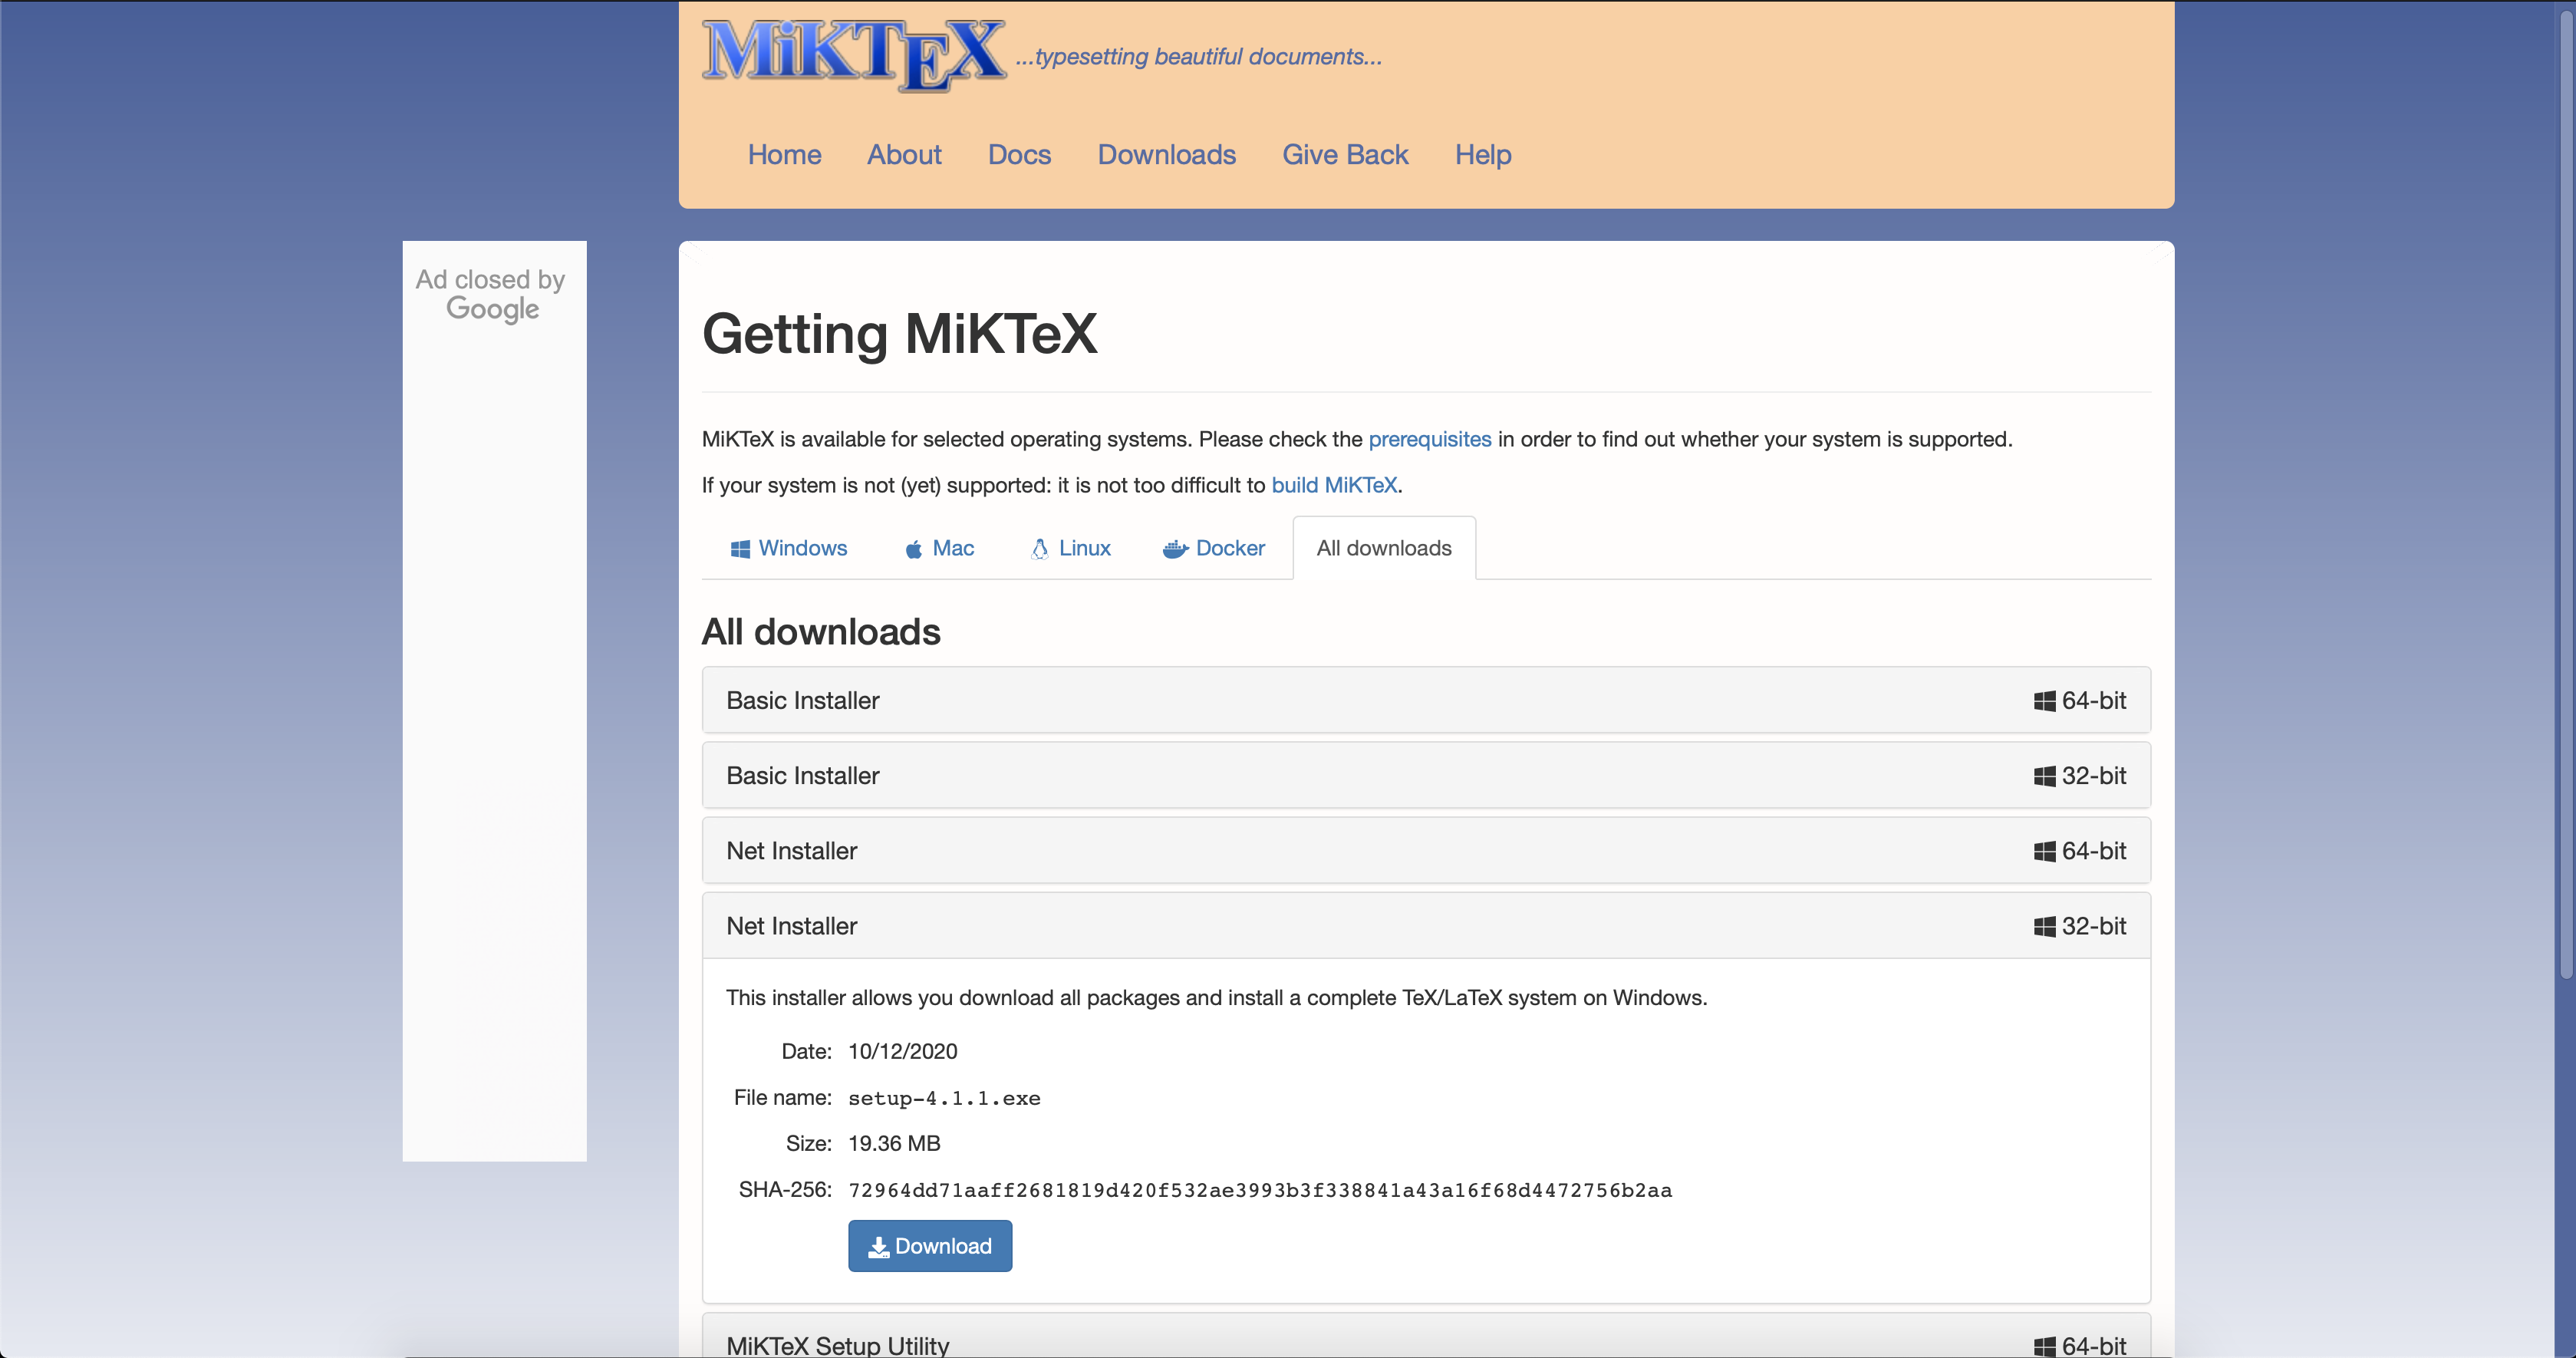
\includegraphics[width=1.0\textwidth]{./fig/miktex10}
  \caption{Instalação  completa do MikTex - Página com net installer.}
  \fontefig{Elaborada pelo autor}
\end{figure}
\item Clique em download para baixar o arquivo de instalação;
\item Abra o instalador e aceite as condições de uso para continuar;
\begin{figure}[H]
  \centering
  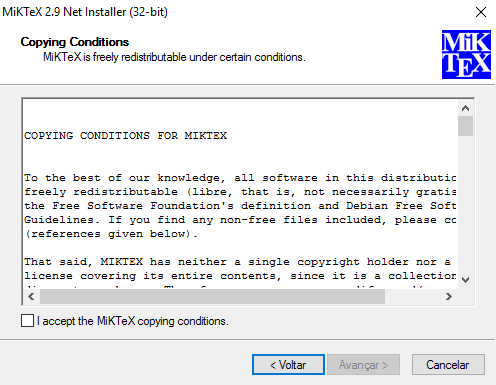
\includegraphics[width=0.6\textwidth]{./fig/miktex11}
  \caption{Instalação completa do MikTex - Primeira página do instalador MikTeX.}
  \fontefig{\cite{miktexfull}}
\end{figure}
\item Baixar o MikTeX;
Agora é possível escolher baixar ou instalar o MikTeX. Escolha a opção de baixar e clique em avançar.
\begin{figure}[H]
  \centering
  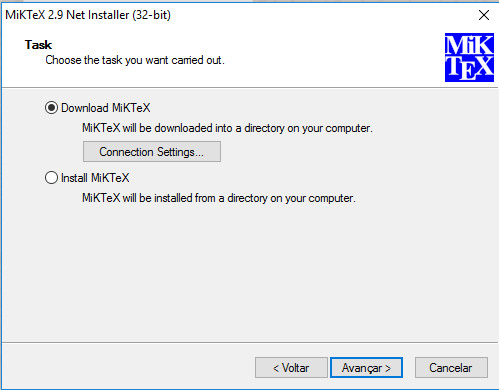
\includegraphics[width=0.6\textwidth]{./fig/miktex12}
  \caption{Instalação completa do MikTex - Segunda tela do instalador do MikTeX.}
  \fontefig{\cite{miktexfull}}
\end{figure}
\item Escolha o tipo de download que deve ser feito.
Escolha qual versão do MikTeX você deseja instalar. O ideal é a instalação completa, que ocupa mais espaço em disco. Se preferir, pode escolher a versão básica para economizar espaço em disco e baixar pacotes adicionais conforme for precisando deles (como na seção anterior). Após escolher uma opção, clique em Avançar.
\begin{figure}[H]
  \centering
  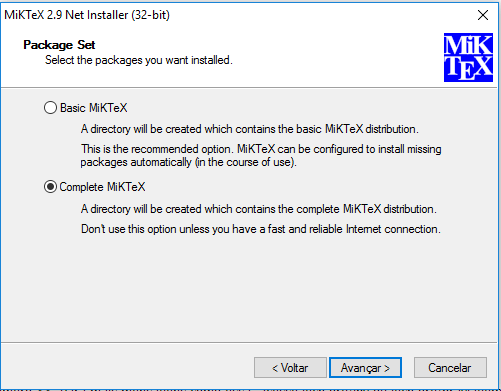
\includegraphics[width=0.6\textwidth]{./fig/miktex13}
  \caption{Instalação completa do MikTex - Tipo de distribuição: básica ou completa.}
  \fontefig{\cite{miktexfull}}
\end{figure}
\item Escolha de onde você deseja baixar.
Nesse passo, é necessário escolher de qual servidor você deseja baixar o MikTeX. É recomendado que você escolha o servidor que estiver mais próximo de onde você estiver acessando a internet. Uma vez escolhido o servidor, o botão Avançar será habilitado e você poderá prosseguir com a instalação.
\begin{figure}[H]
  \centering
  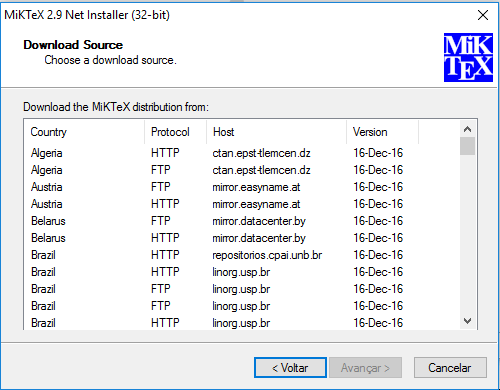
\includegraphics[width=0.6\textwidth]{./fig/miktex14}
  \caption{Instalação completa do MikTex - Lista de servidores que permitem o download do MikTeX.}
  \fontefig{\cite{miktexfull}}
\end{figure}
\item Escolha o local do seu computador onde os arquivos devem ser salvos.
Agora é necessário que você determine uma pasta do seu computador para que os arquivos sejam baixados. É importante que seja um local fácil, já que posteriormente será necessário indicar para o instalador do MikTeX essa mesma pasta para que a instalação seja iniciada. Uma vez escolhida uma pasta, basta continuar.
\begin{figure}[H]
  \centering
  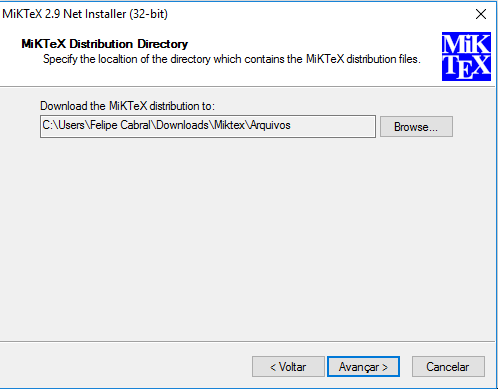
\includegraphics[width=0.6\textwidth]{./fig/miktex15}
  \caption{Instalação completa do MikTex - Determine o local onde os arquivos devem ser salvos em seu computador.}
  \fontefig{\cite{miktexfull}}
\end{figure}
\item Revise suas opções e inicie o download.
Se estiver tudo certo, clique em \textbf{Start} e o download será iniciado. Assim que terminar o download, você poderá finalizar o instalador.
\begin{figure}[H]
  \centering
  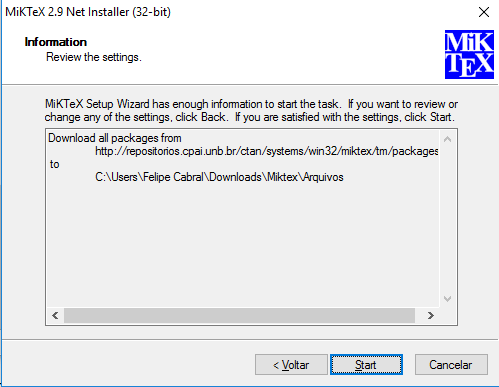
\includegraphics[width=0.6\textwidth]{./fig/miktex16}
  \caption{Instalação completa do MikTex - Resumo das opções escolhidas para iniciar o download.}
  \fontefig{\cite{miktexfull}}
\end{figure}
\item Instalação do MikTeX.
Uma vez terminado o download, é necessário dar início ao processo de instalação do MikTeX. Para isso, abra novamente o instalador e escolha a opção \textbf{Install MikTeX} para que o processo de instalação se inicie.
\begin{figure}[H]
  \centering
  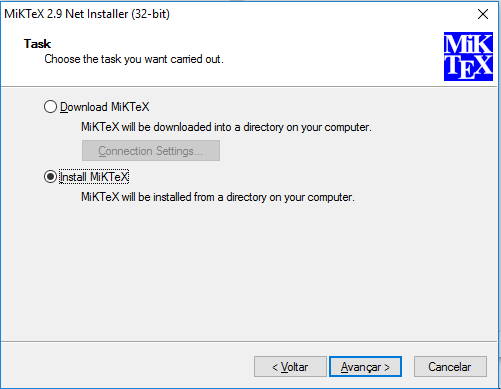
\includegraphics[width=0.6\textwidth]{./fig/miktex17}
  \caption{Instalação completa do MikTex - Instalação do MikTeX após o download concluído.}
  \fontefig{\cite{miktexfull}}
\end{figure}
\item Escolha o tipo de distribuição.
\begin{figure}[H]
  \centering
  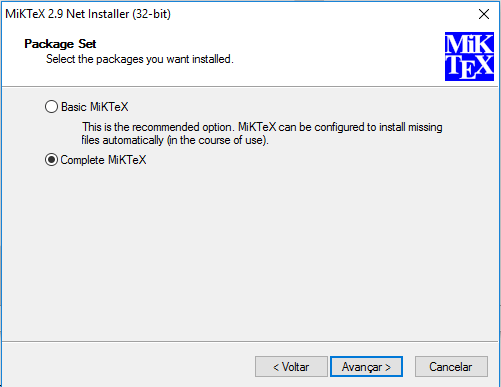
\includegraphics[width=0.6\textwidth]{./fig/miktex18}
  \caption{Instalação completa do MikTex - Escolha entre a versão básica e a completa. Basta escolher a que você baixou.}
  \fontefig{\cite{miktexfull}}
\end{figure}
\item Escolha a pasta onde o download do MikTeX foi realizado.
Nesse momento, é necessário escolher a pasta onde o download do MikTeX foi realizado. Geralmente, o instalador preenche o caminho para a pasta escolhida automaticamente, mas você pode alterar a pasta clicando em \textbf{Browse} caso o caminho esteja errado.
\begin{figure}[H]
  \centering
  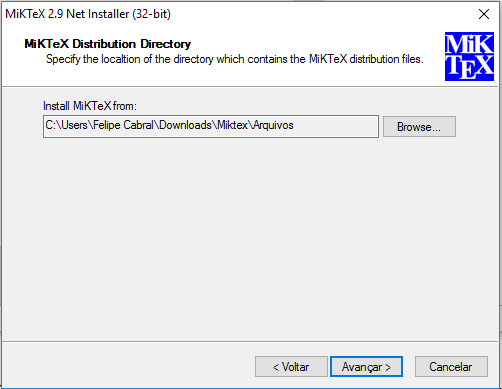
\includegraphics[width=0.6\textwidth]{./fig/miktex19}
  \caption{Instalação completa do MikTex - Escolha a pasta onde o MikTeX foi baixado.}
  \fontefig{\cite{miktexfull}}
\end{figure}
\item Escolha o local de instalação.
Finalmente, escolha o local onde o MikTeX deve ser instalado em seu computador e prossiga com a instalação. 
\begin{figure}[H]
  \centering
  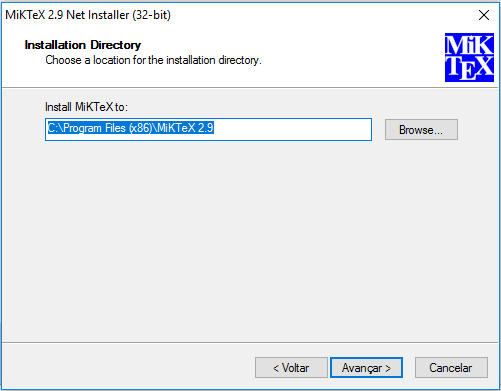
\includegraphics[width=0.6\textwidth]{./fig/miktex20}
  \caption{Instalação completa do MikTex - Local onde o MikTeX será instalado em seu computador.}
  \fontefig{\cite{miktexfull}}
\end{figure}
\end{enumerate}

\section{Instalando o editor}

Para realizar a edição de documentos \LaTeX\ no computador, além do compilador MikTex é necessário instalar o editor. Neste documento, para o sistema operacional Windows é sugerido o uso do TeXnicCenter, cuja instalação é detalhada a seguir \cite{texnic}.

\begin{enumerate}
\item Faça o download do arquivo de instalação disponível em \url{https://www.texniccenter.org/download/}. Selecione a opção de acordo com a versão do seu sistema operacional. 
\item Abra o arquivo baixado.
\item Se uma janela de aviso de segurança for aberta apenas clique na opção \aspas{Executar} para prosseguir a instalação, caso contrário vá para o passo seguinte.
\begin{figure}[H]
  \centering
  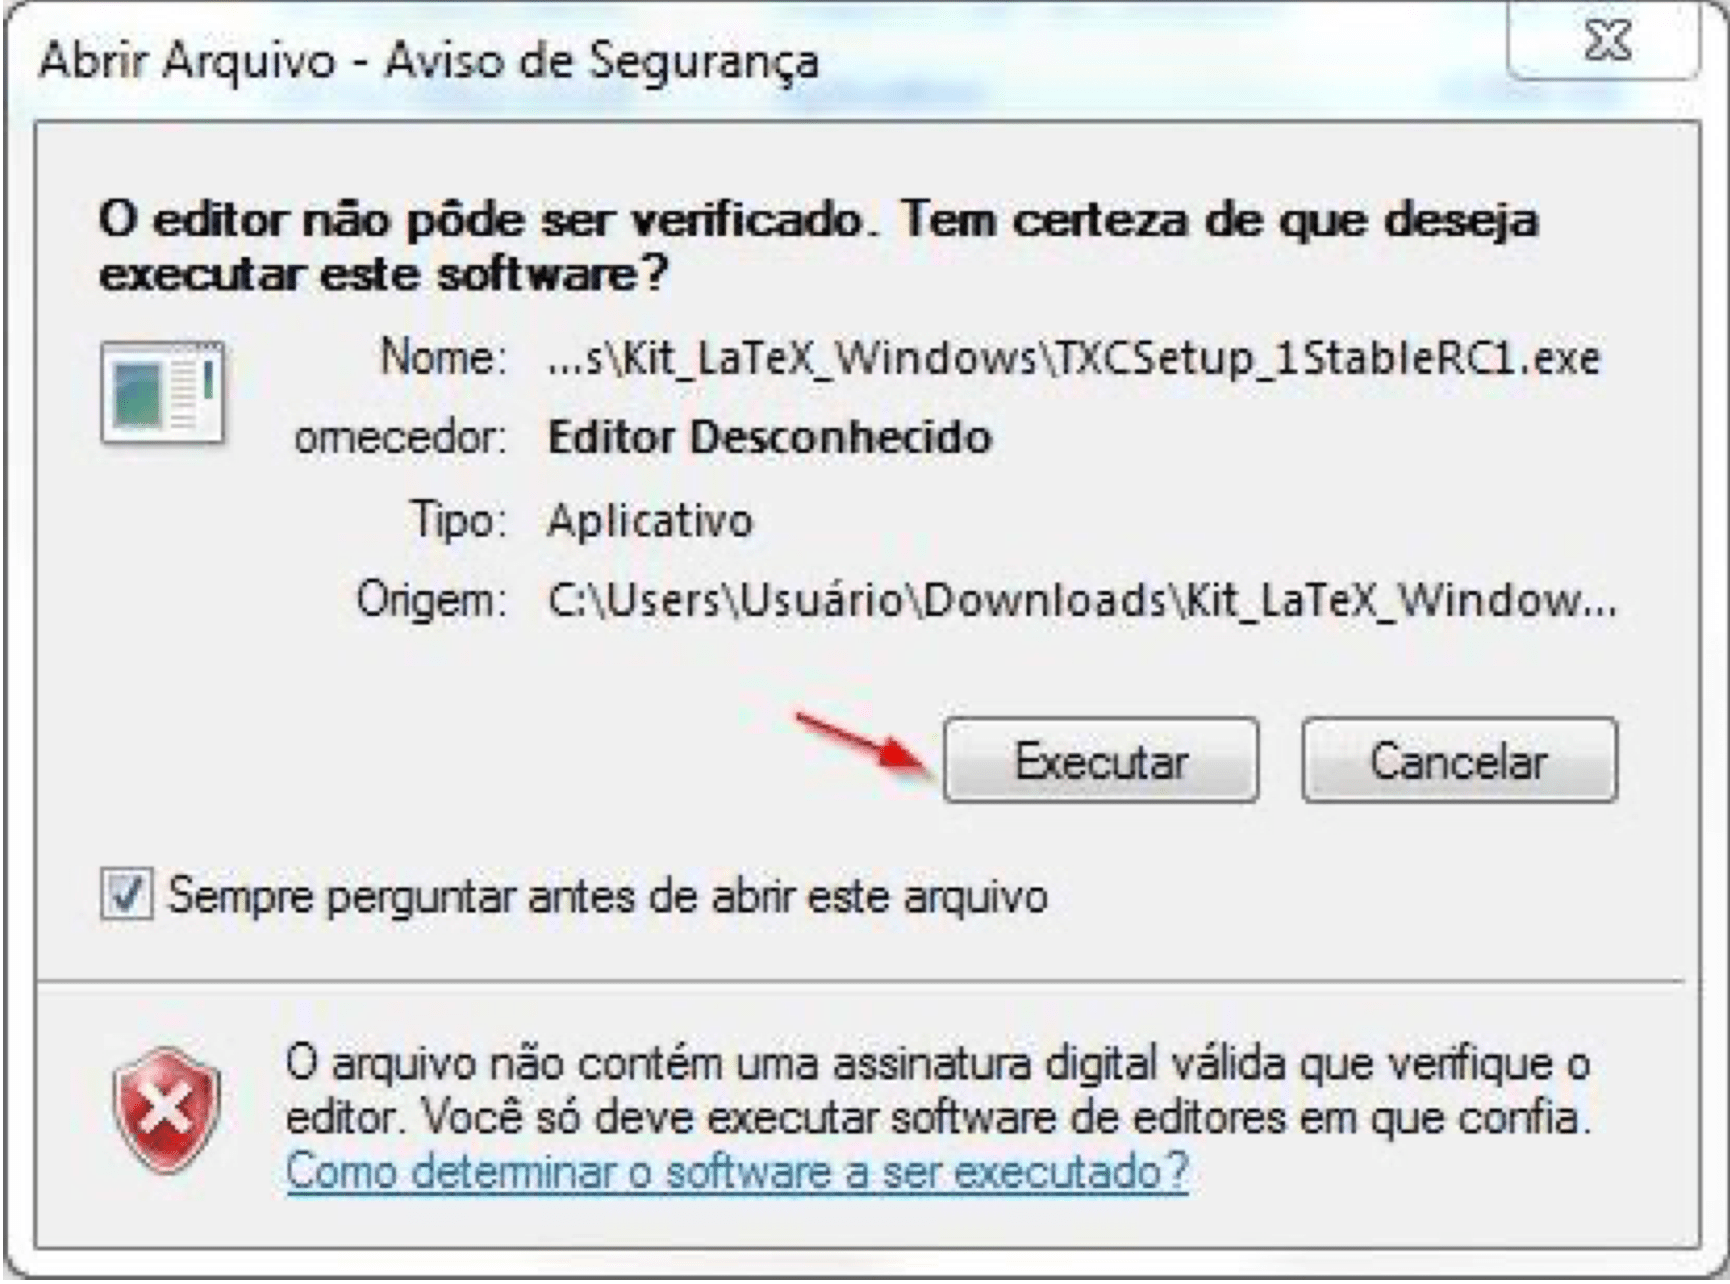
\includegraphics[width=0.6\textwidth]{./fig/texniccenter01}
  \caption{Instalação do TeXnicCenter - Aviso de segurança.}
  \fontefig{\cite{texnic}}
\end{figure}
\item Para iniciar o processo de instalação na tela exibida clique no botão \textbf{Next}.
\begin{figure}[H]
  \centering
  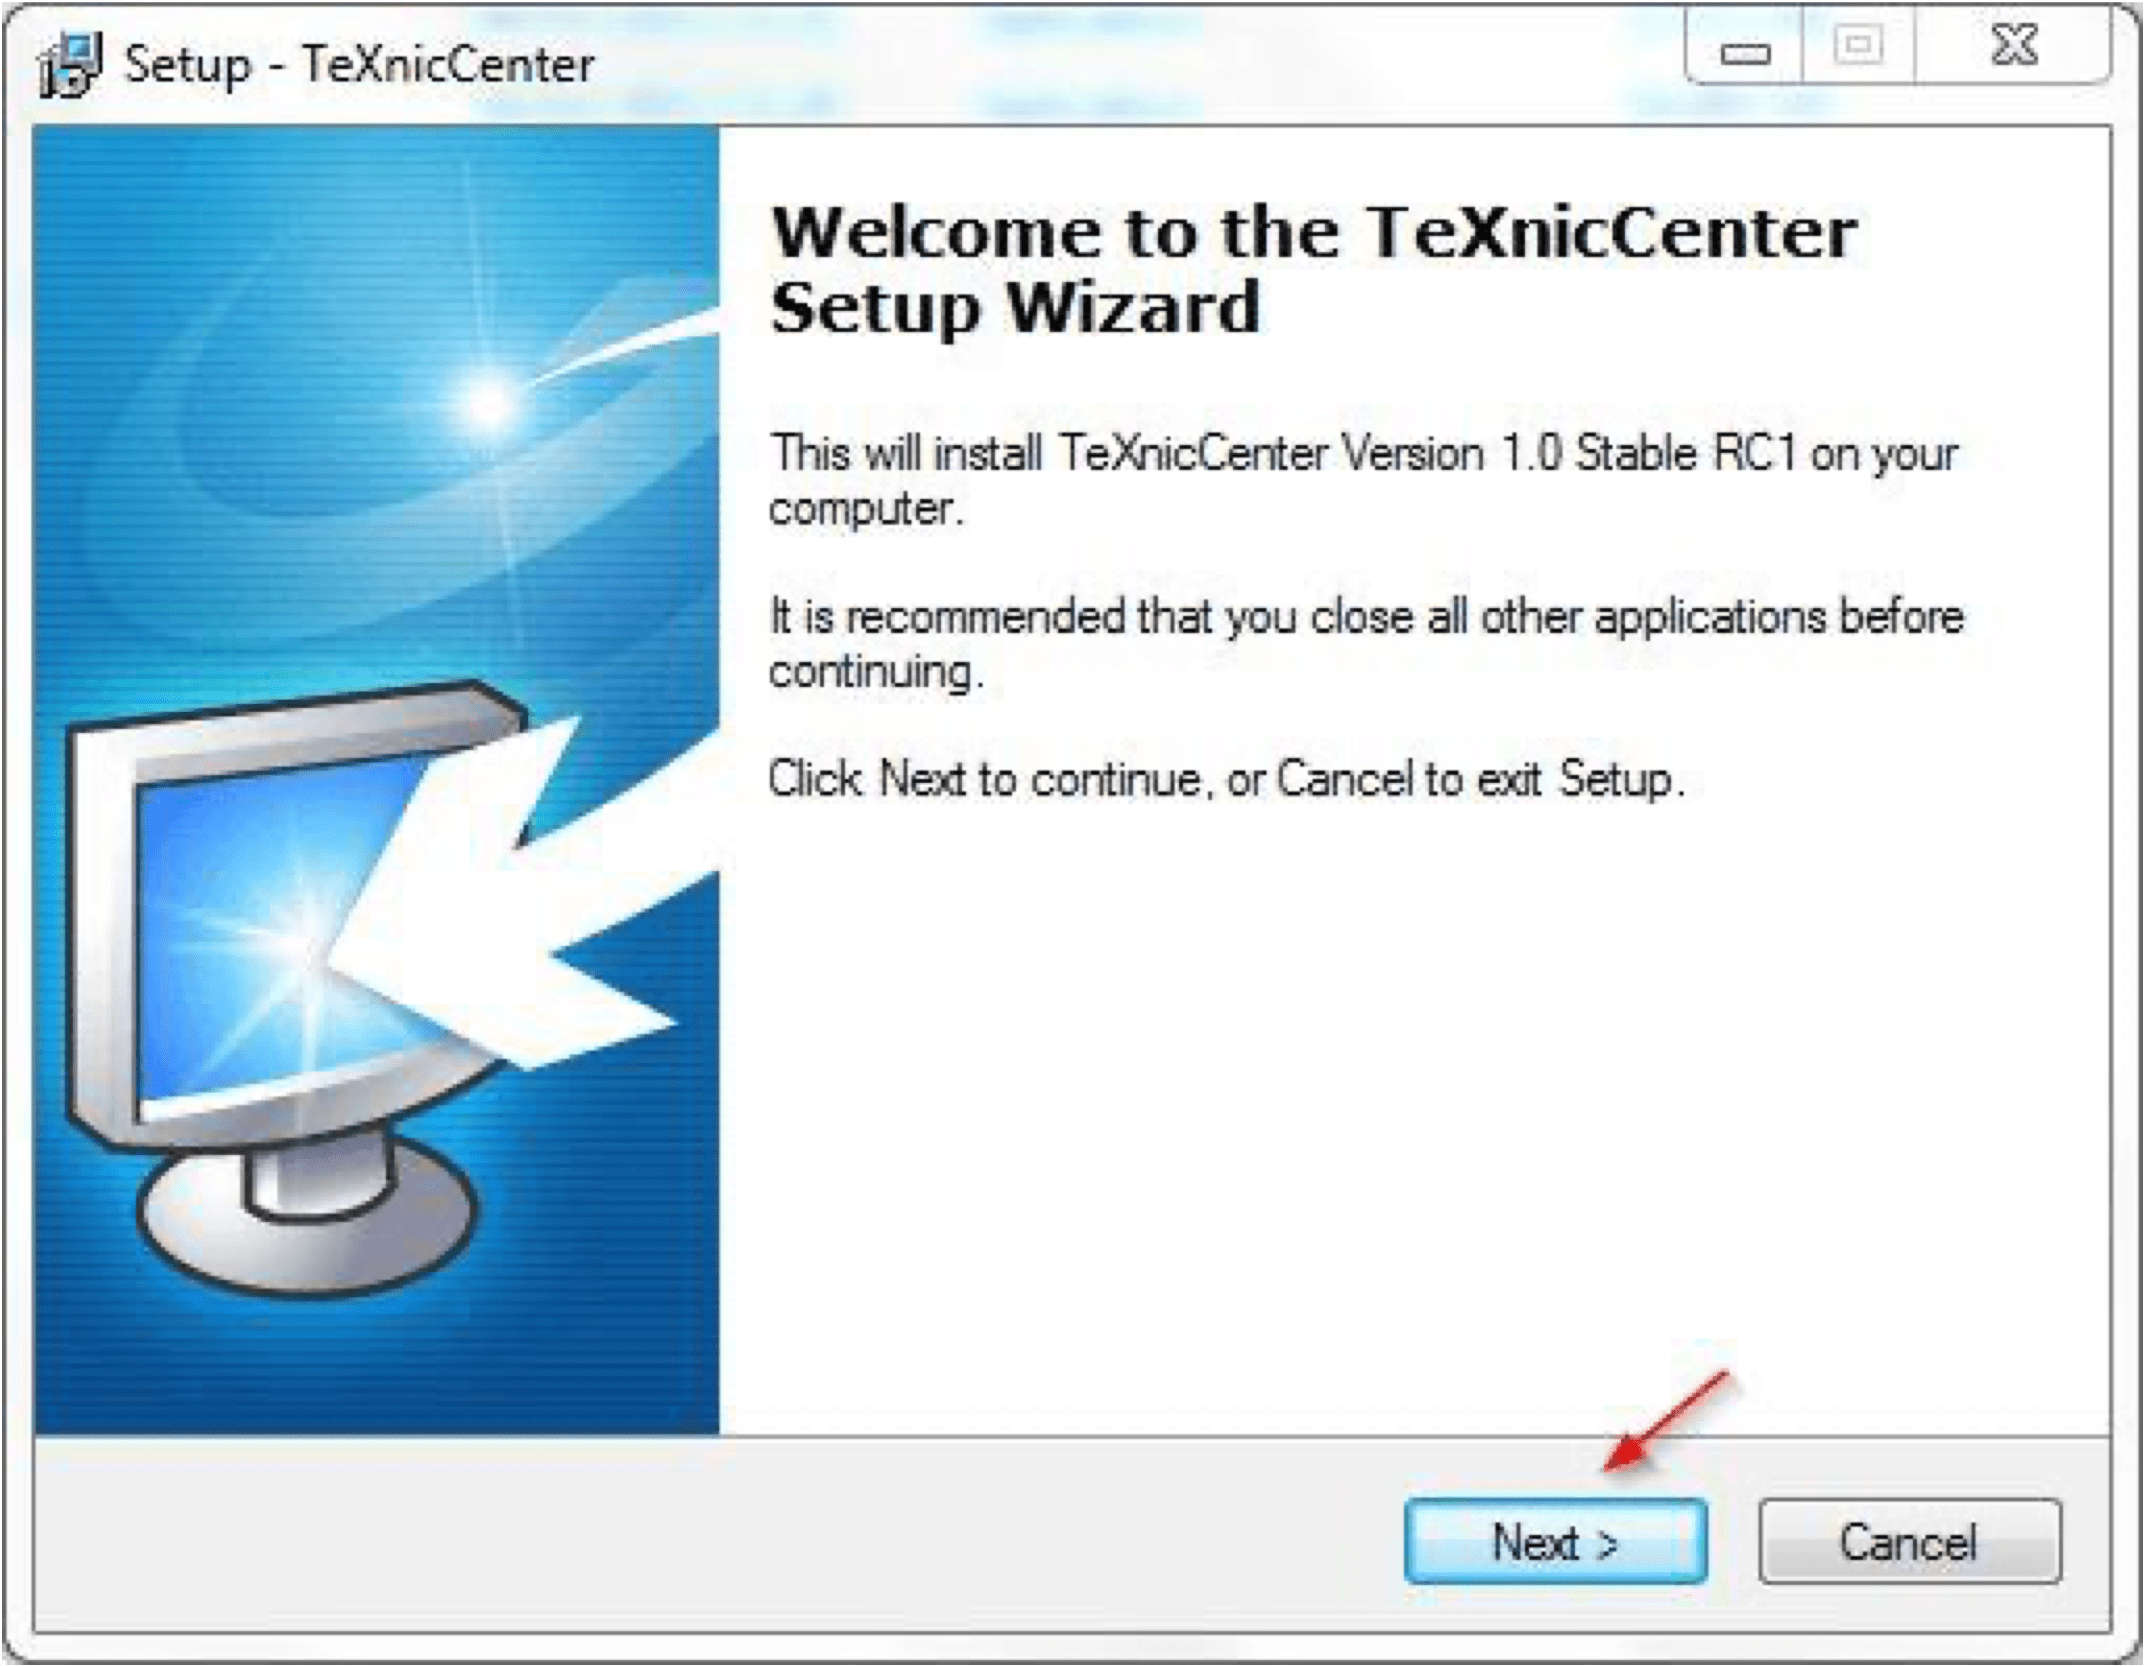
\includegraphics[width=0.6\textwidth]{./fig/texniccenter02}
  \caption{Instalação do TeXnicCenter - Primeira tela.}
  \fontefig{\cite{texnic}}
\end{figure}
\item É necessário aceitar a licença de uso do software selecionando a opção \textbf{I accept the agreement}.
\begin{figure}[H]
  \centering
  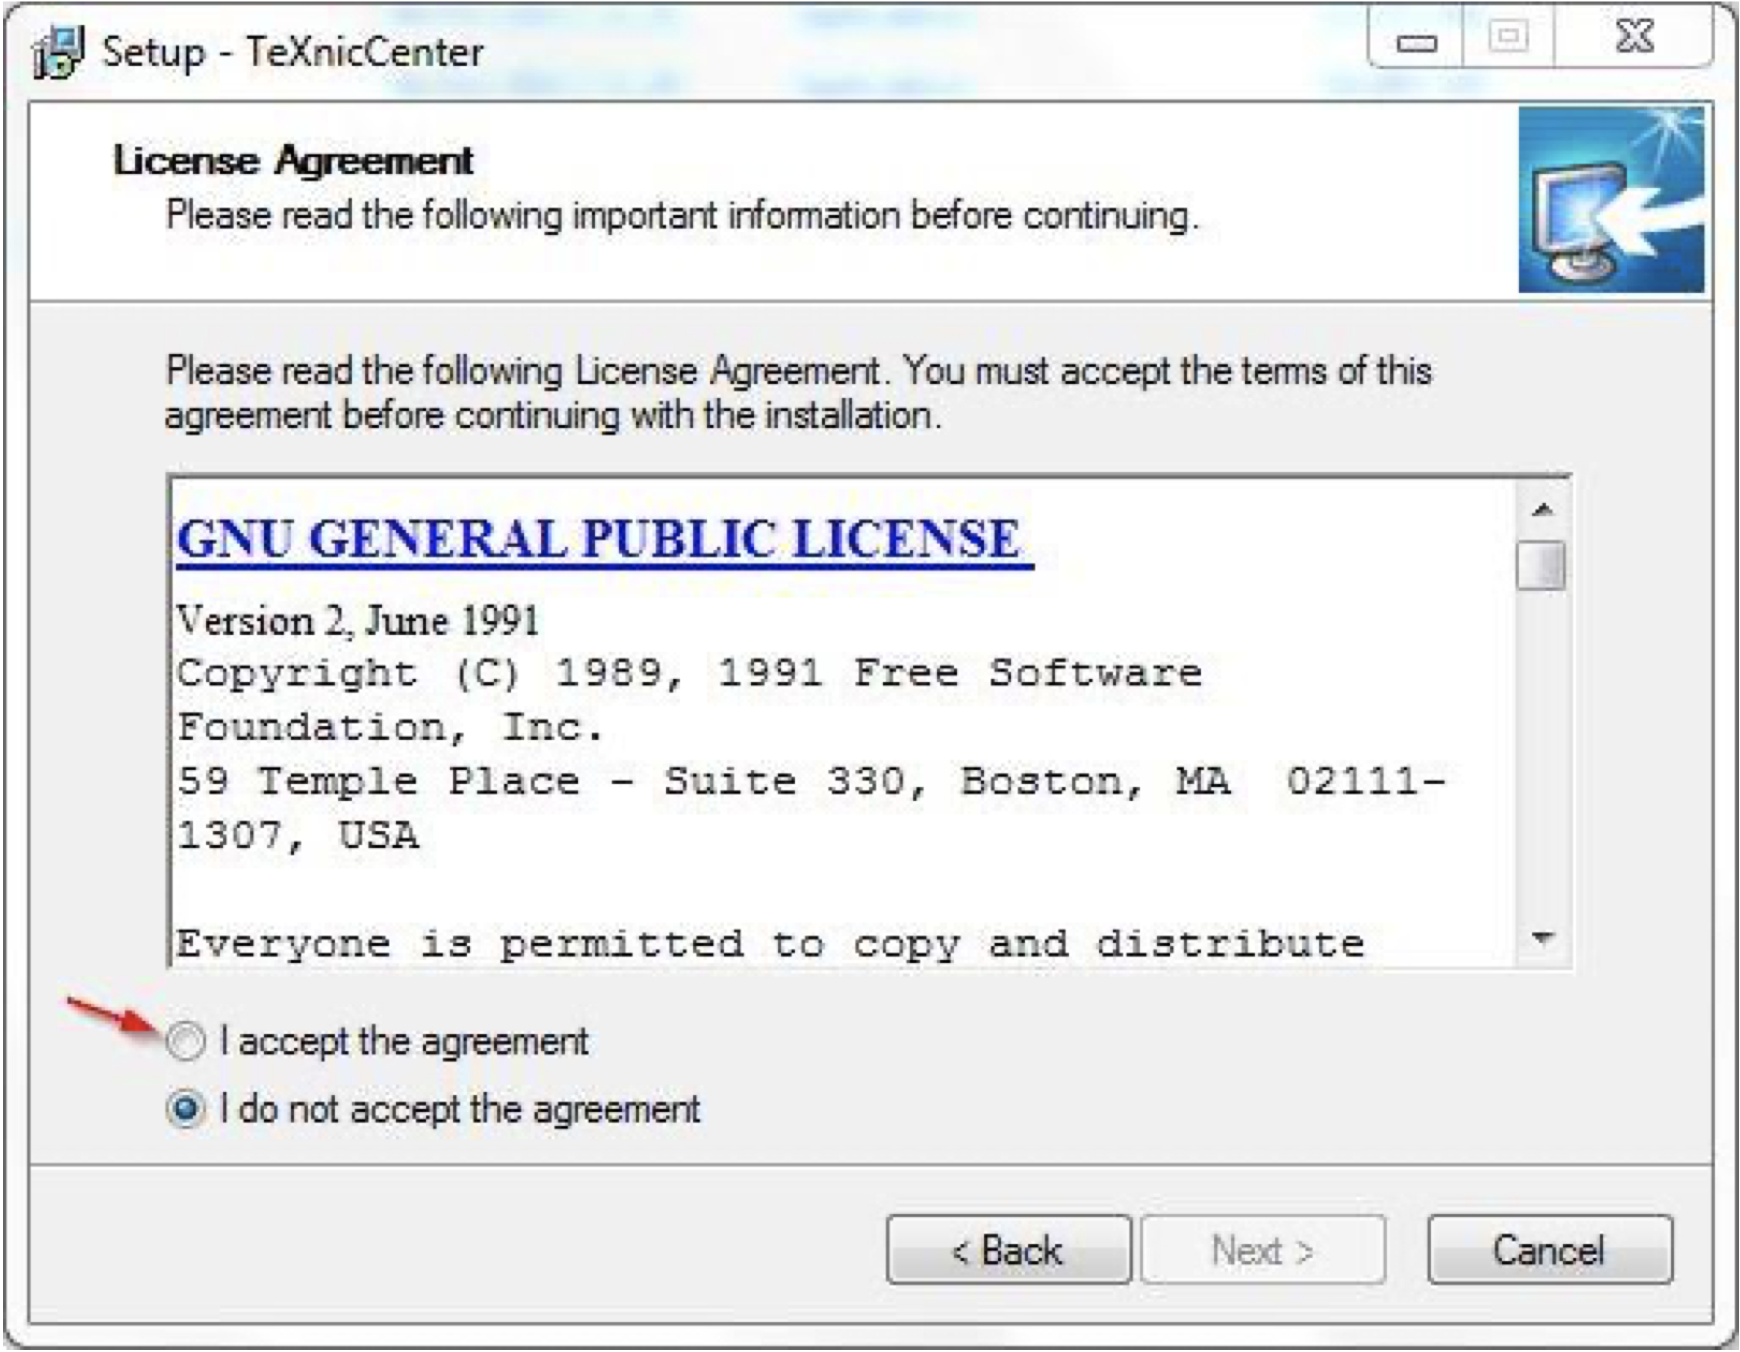
\includegraphics[width=0.6\textwidth]{./fig/texniccenter03}
  \caption{Instalação do TeXnicCenter - Segunda tela.}
  \fontefig{\cite{texnic}}
\end{figure}
\item Após aceitar a licença do software clique no botão \textbf{Next}.
\begin{figure}[H]
  \centering
  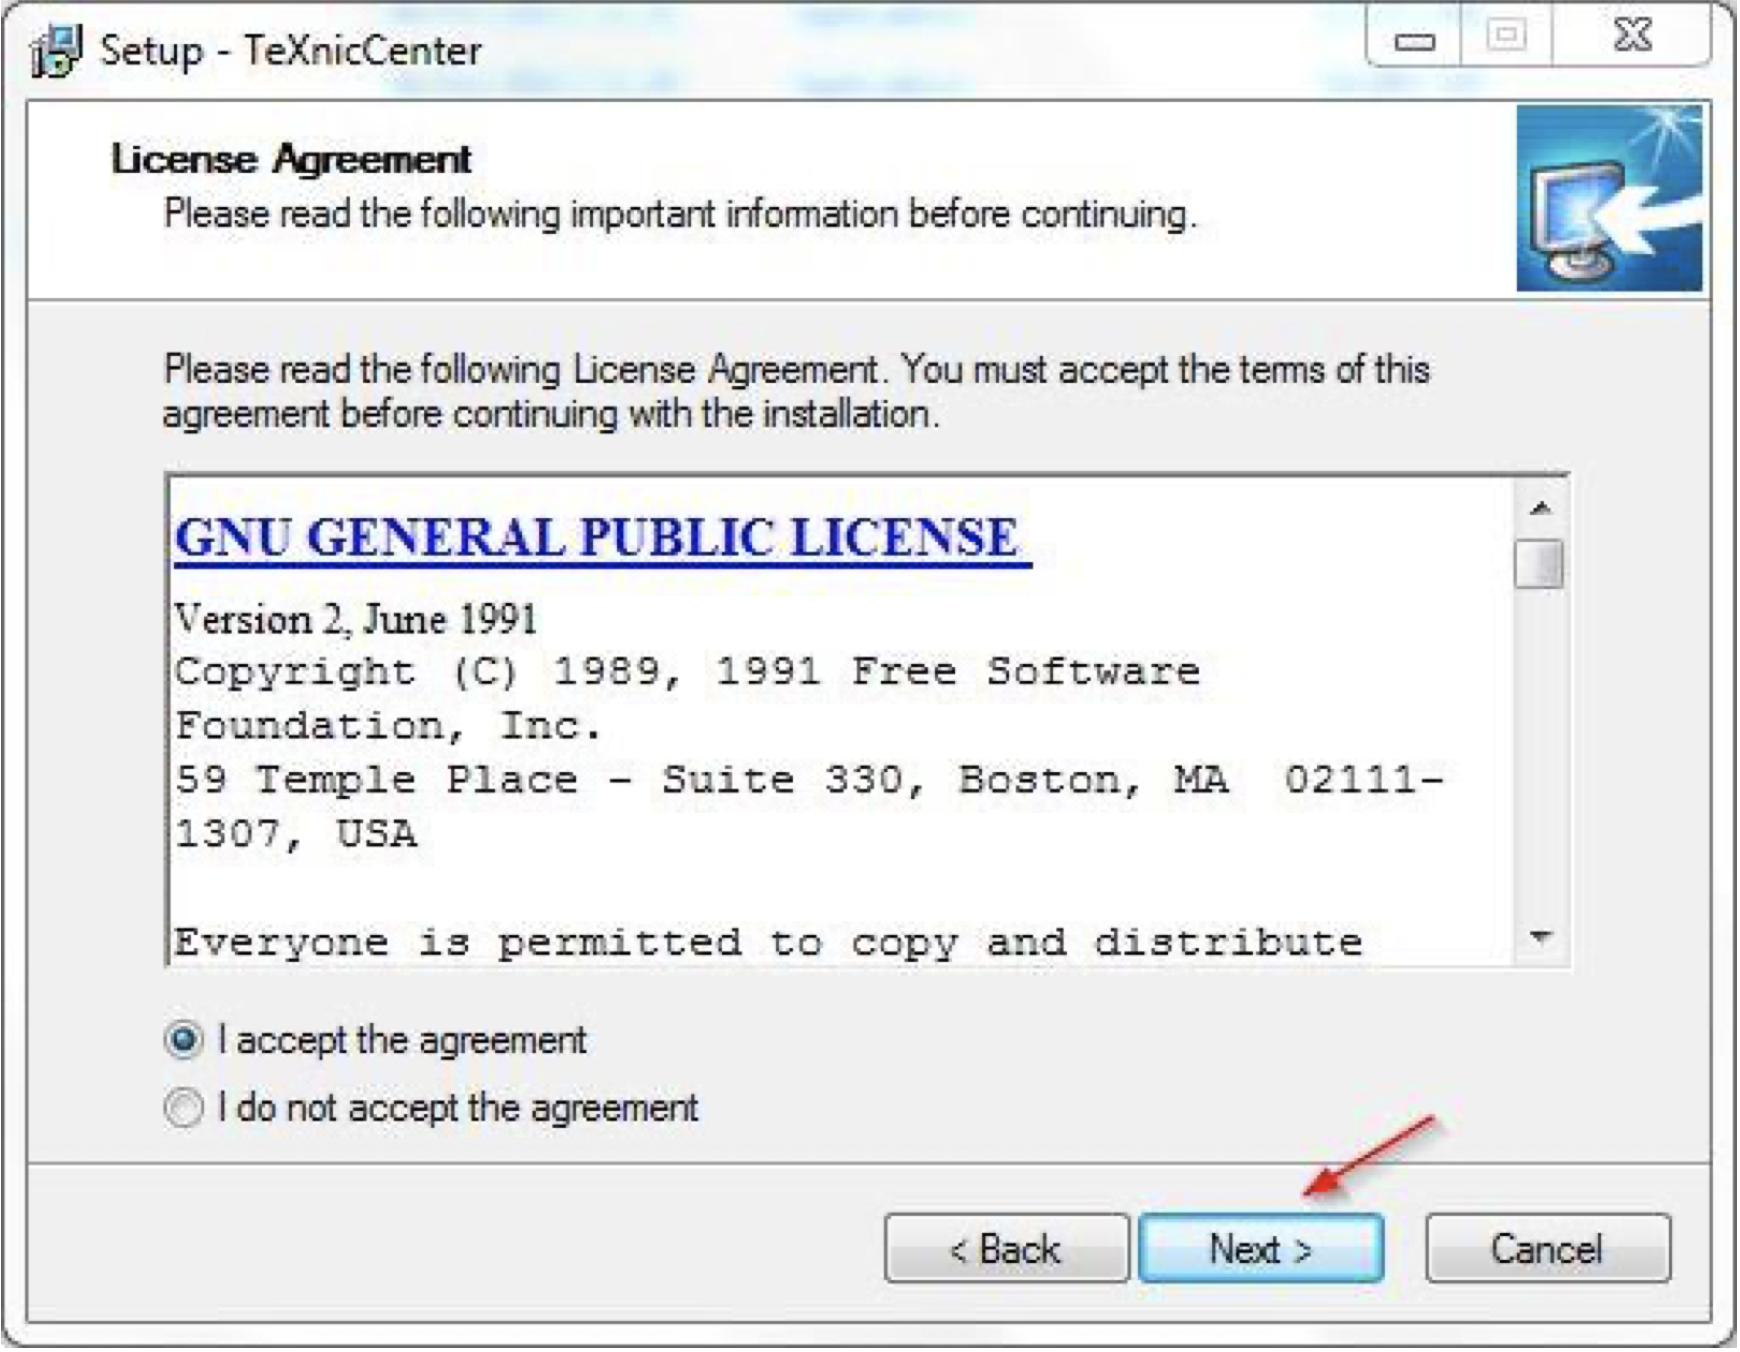
\includegraphics[width=0.6\textwidth]{./fig/texniccenter04}
  \caption{Instalação do TeXnicCenter - Segunda tela (após aceitar termos).}
  \fontefig{\cite{texnic}}
\end{figure}
\item Agora é apresentado o local onde o software será instalado, não é necessário selecionar outra pasta, copie o local indicado como padrão (neste tutorial é o: \aspas{C:$\backslash$Program Files (x86)$\backslash$TeXnicCenter}, mas pode variar dependendo da versão do Windows utilizado) para posteriormente instalar o corretor ortográfico Vero. Clique em \textbf{Next} para continuar o processo de instalação.
\begin{figure}[H]
  \centering
  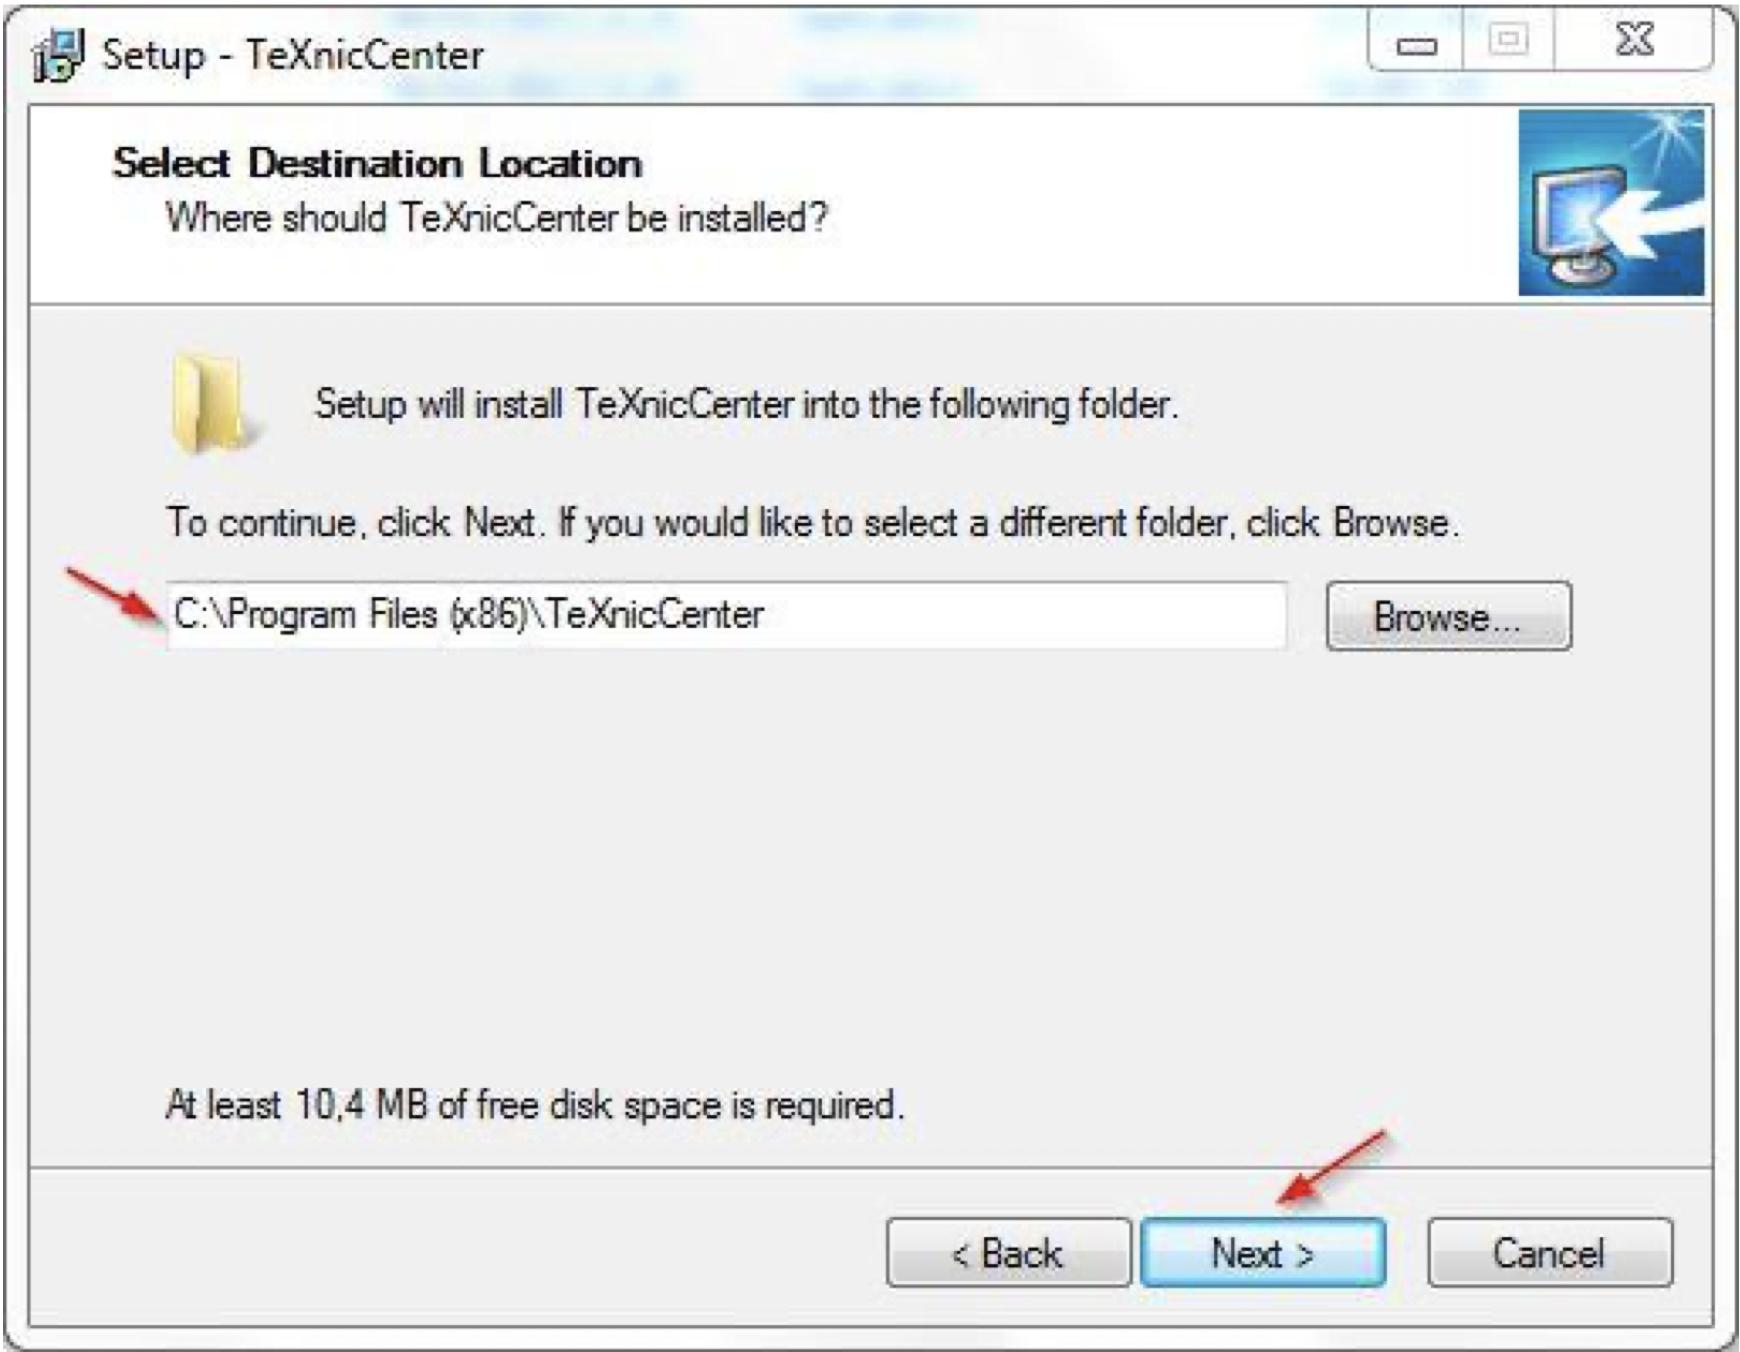
\includegraphics[width=0.6\textwidth]{./fig/texniccenter05}
  \caption{Instalação do TeXnicCenter - Terceira tela.}
  \fontefig{\cite{texnic}}
\end{figure}
\item A tela de seleção de componentes será exibida, não será necessário selecionar nenhuma opção apenas mantenha as opções selecionadas por padrão e clique no botão \textbf{Next} para continuar o processo.
\begin{figure}[H]
  \centering
  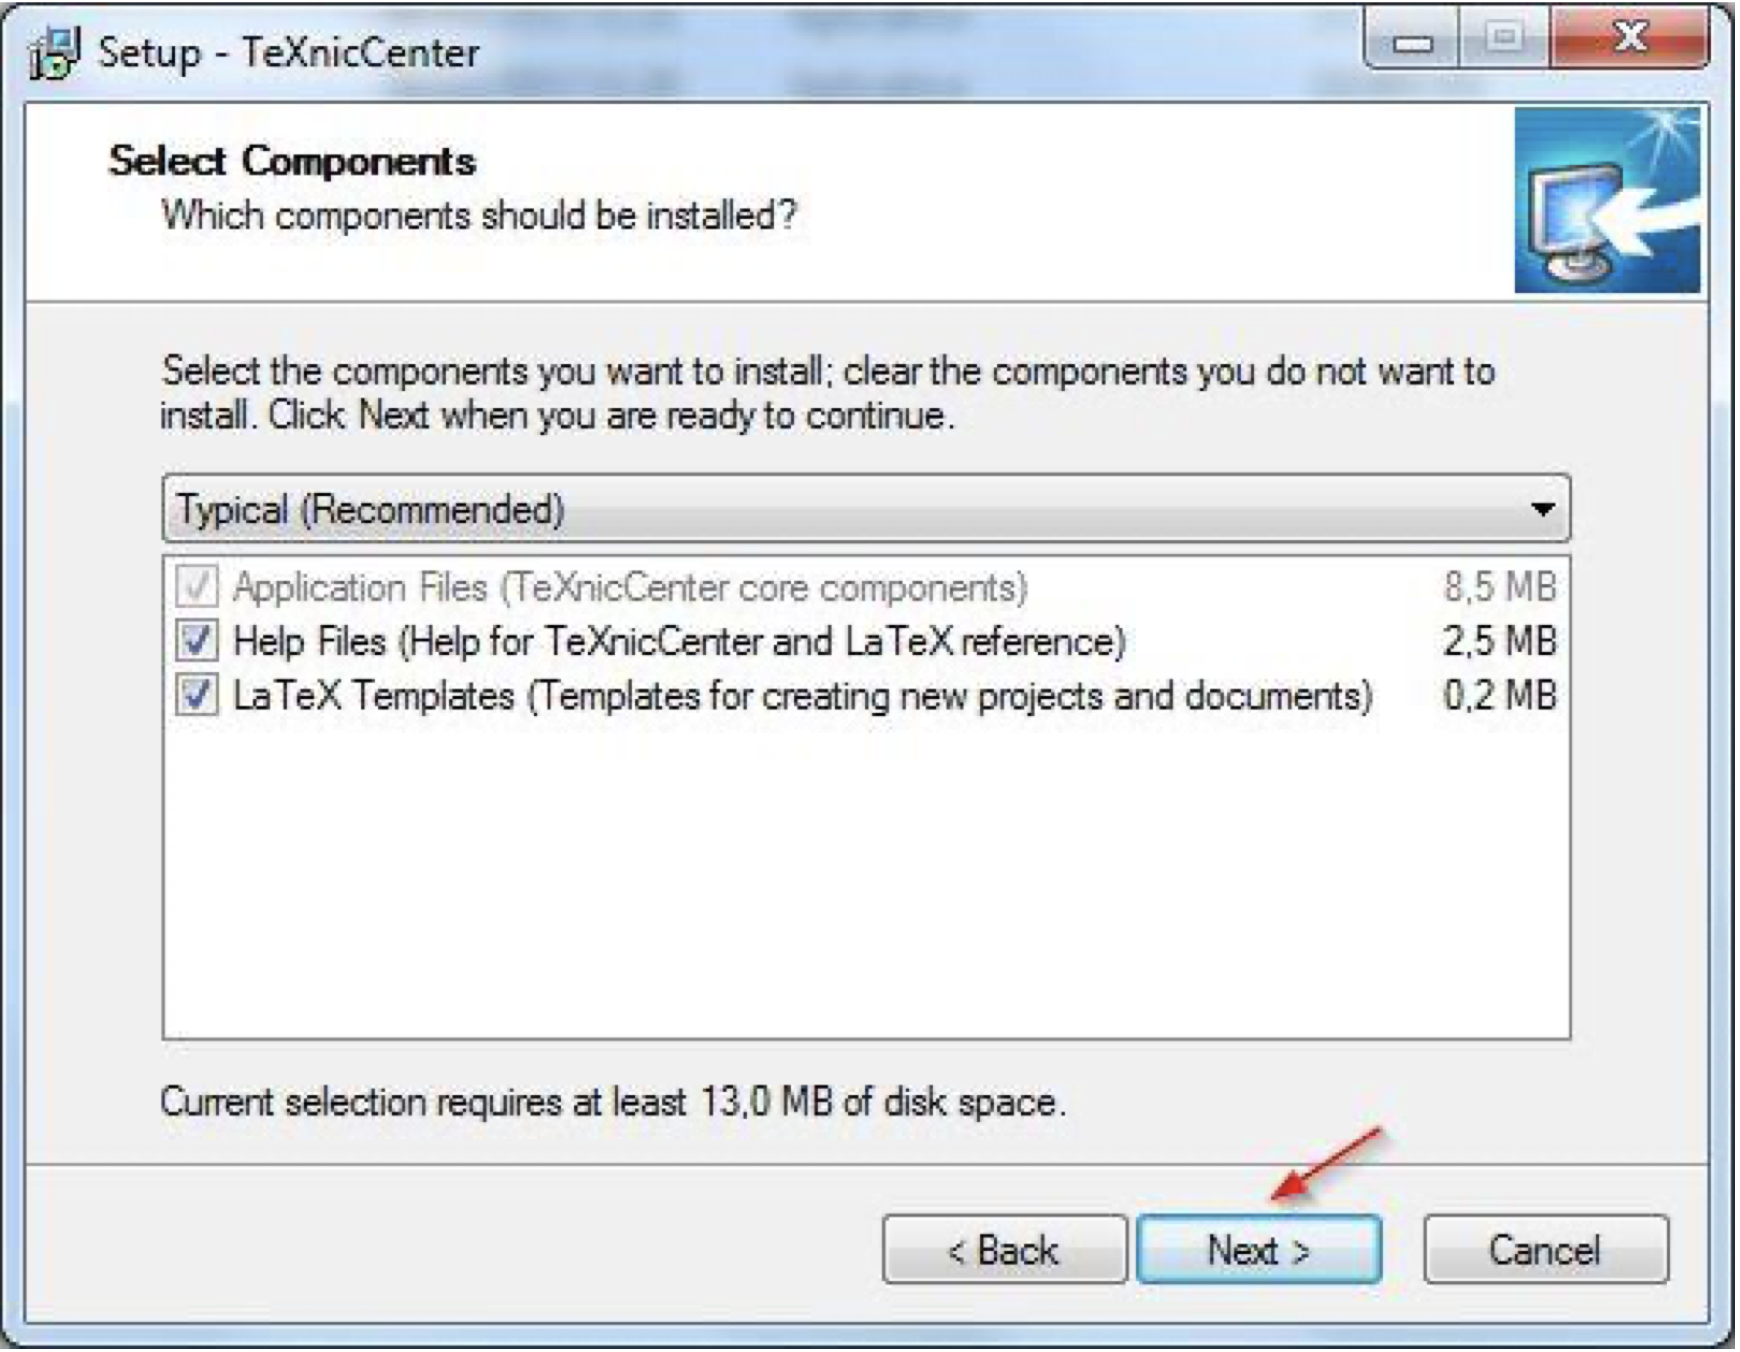
\includegraphics[width=0.6\textwidth]{./fig/texniccenter06}
  \caption{Instalação do TeXnicCenter - Quarta tela.}
  \fontefig{\cite{texnic}}
\end{figure}
\item Agora será exibida a opção para a criação os ícones do software no menu do Windows, apenas clique em \textbf{Next}.
\begin{figure}[H]
  \centering
  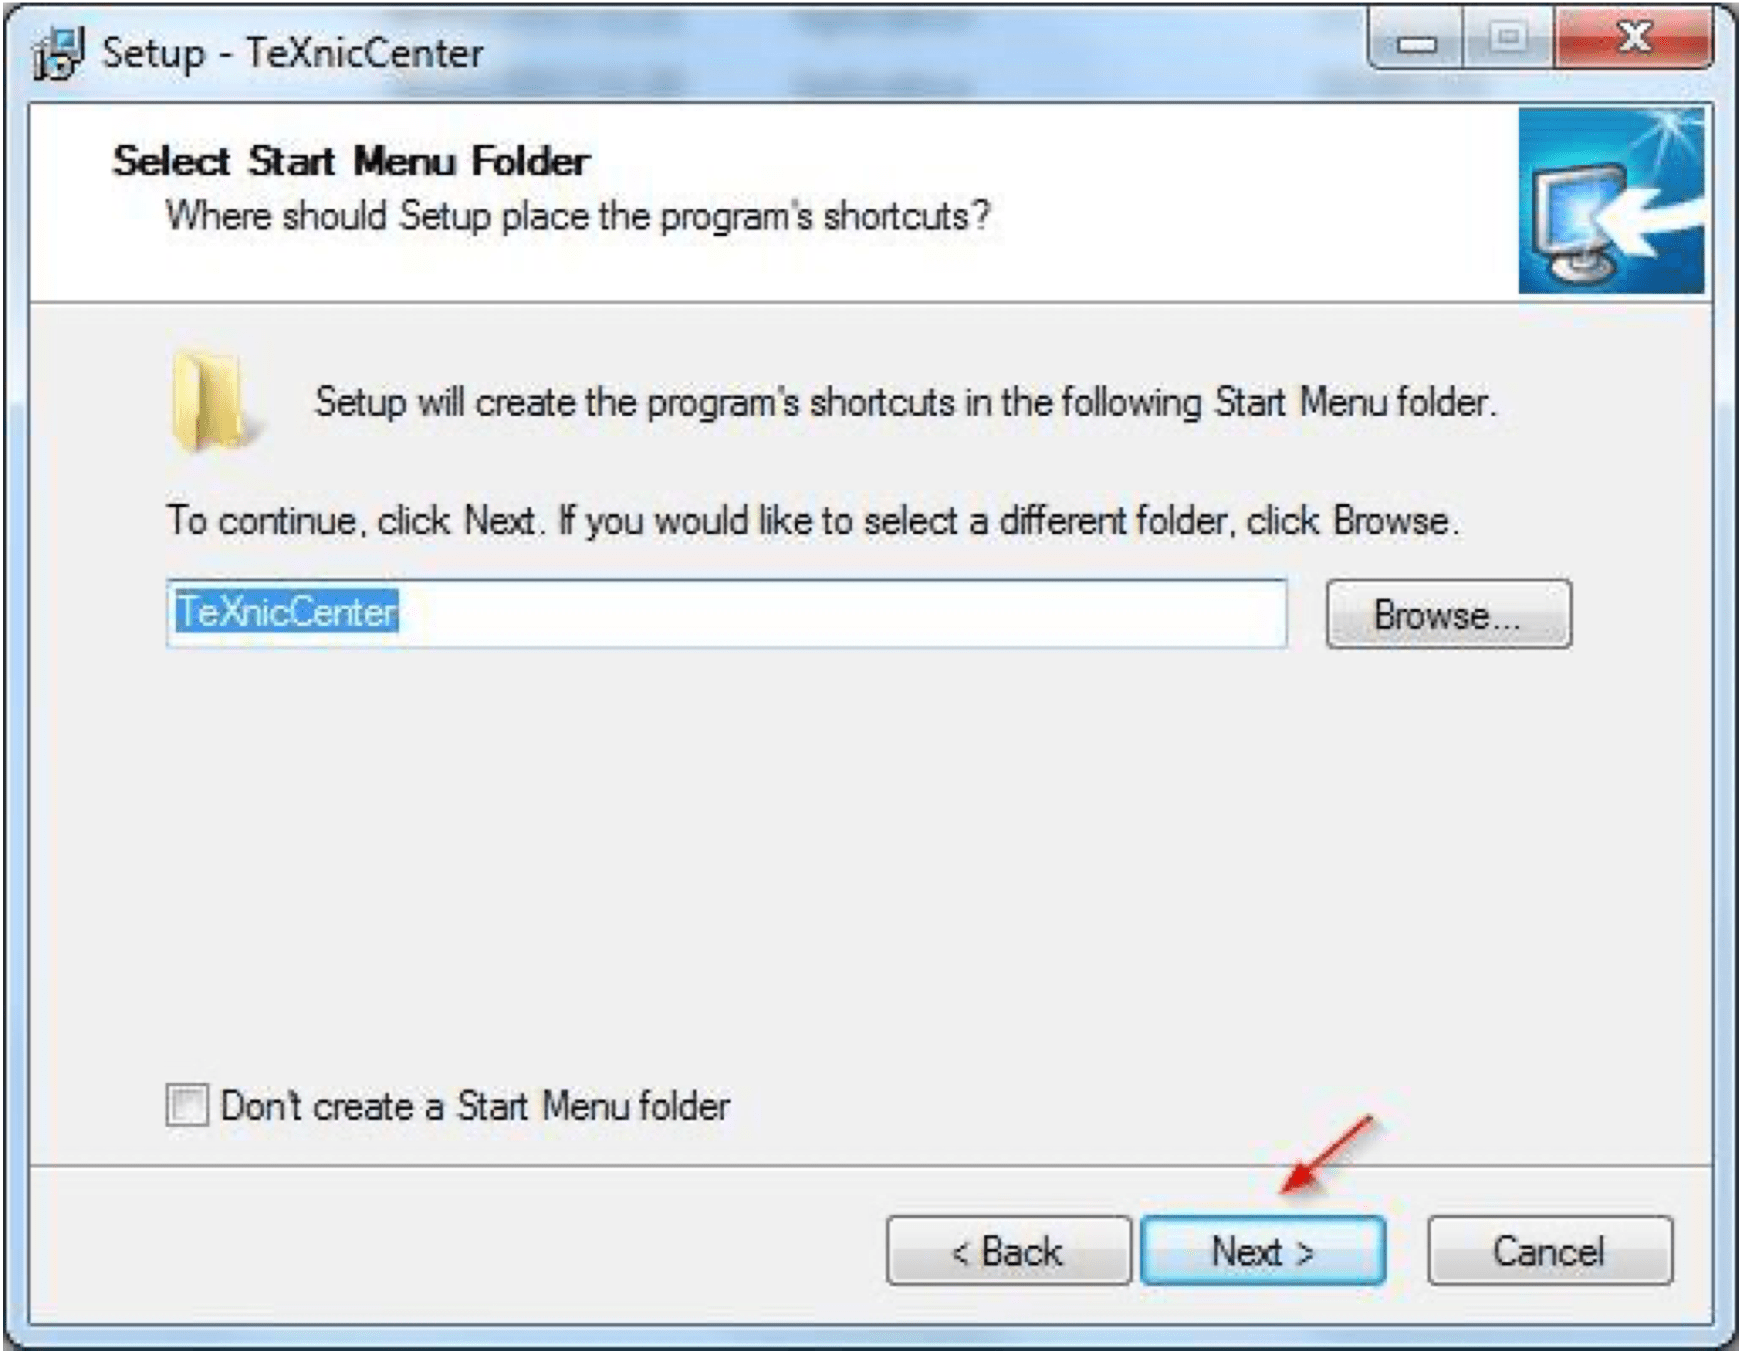
\includegraphics[width=0.6\textwidth]{./fig/texniccenter07}
  \caption{Instalação do TeXnicCenter - Quinta tela.}
  \fontefig{\cite{texnic}}
\end{figure}
\item Serão exibidas as opções para a criação de ícones adicionais para acesso ao software, apenas clique em \textbf{Next} para continuar.
\begin{figure}[H]
  \centering
  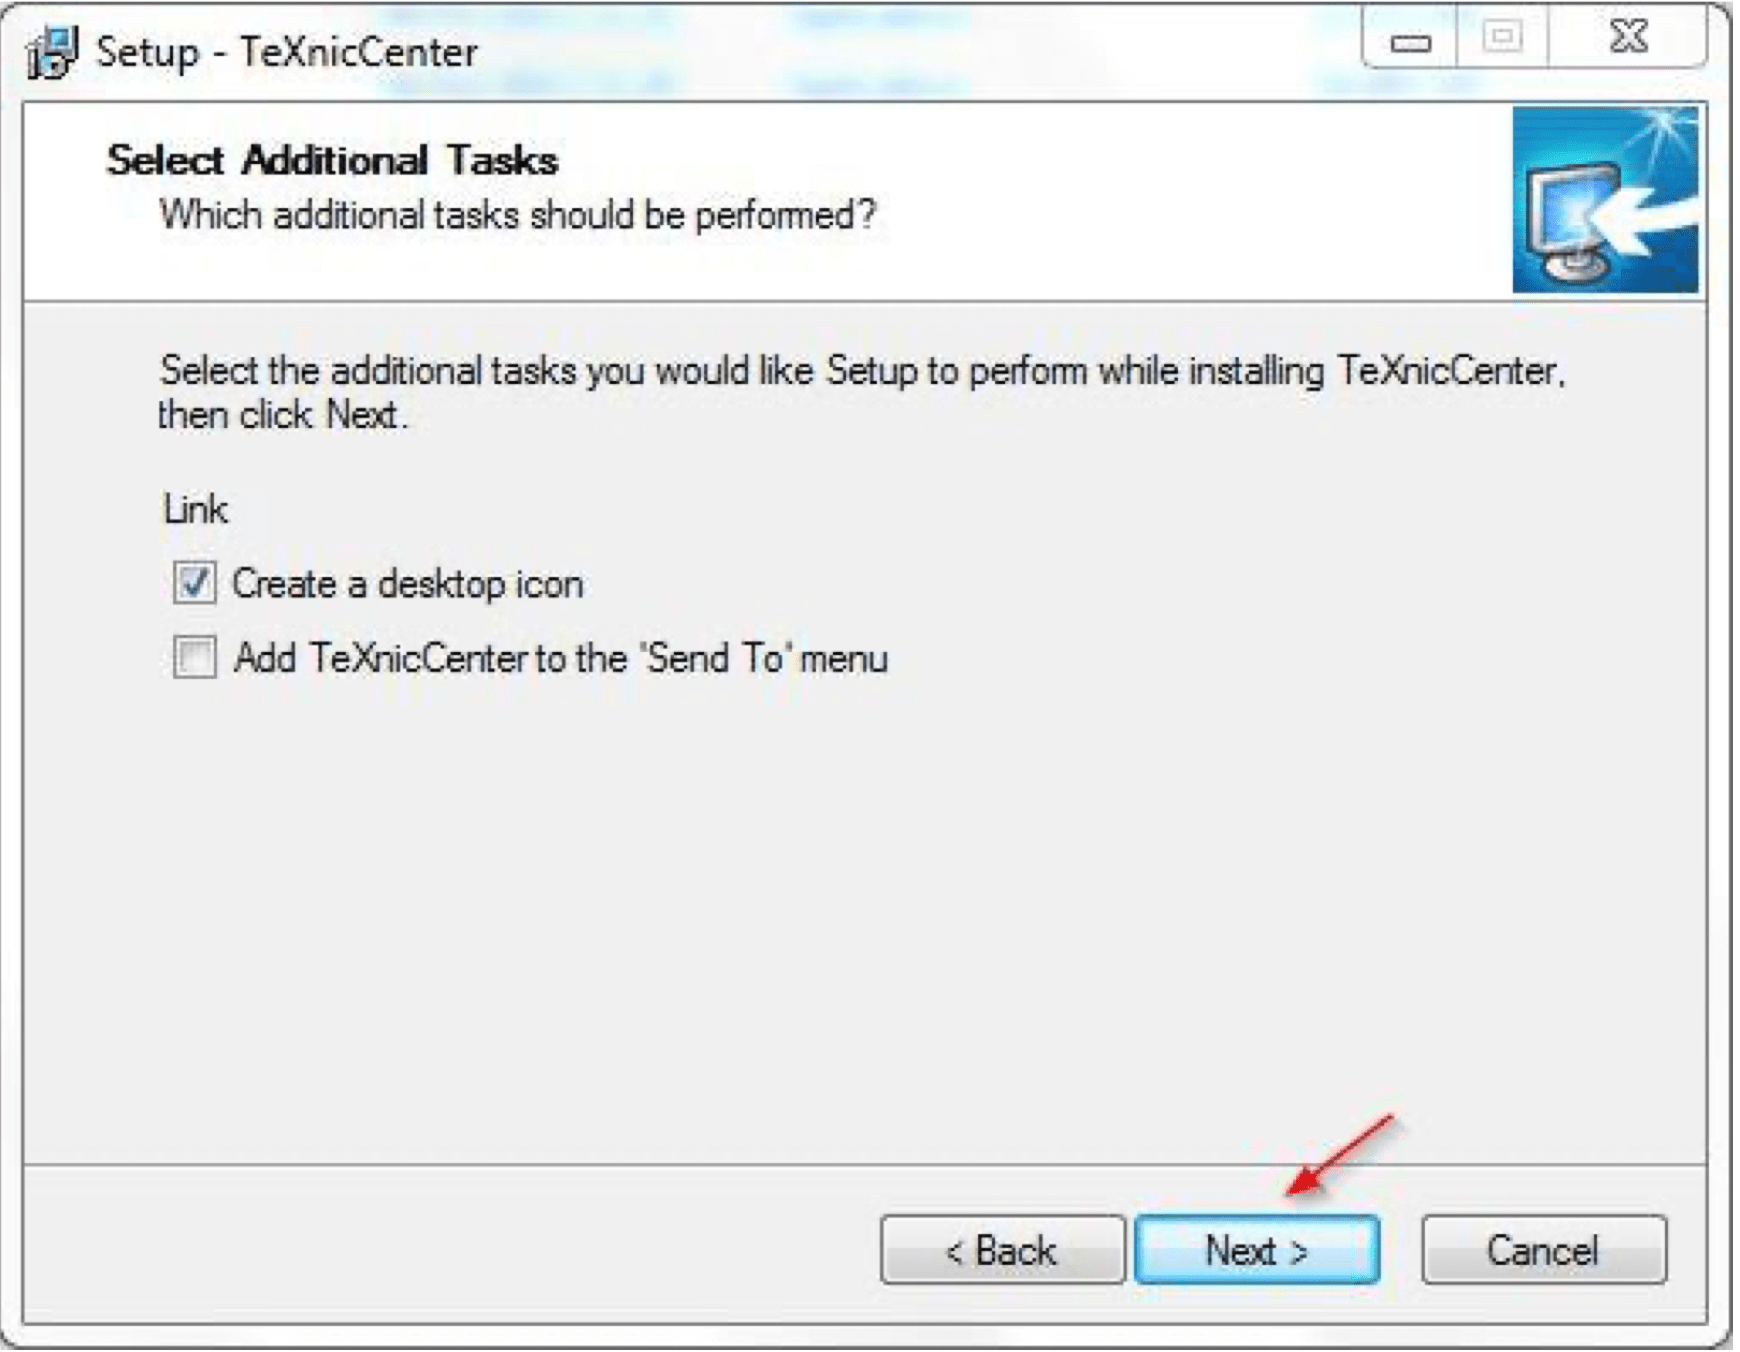
\includegraphics[width=0.6\textwidth]{./fig/texniccenter08}
  \caption{Instalação do TeXnicCenter - Sexta tela.}
  \fontefig{\cite{texnic}}
\end{figure}
\item Um resumo com as opções anteriormente selecionadas será exibido, clique em \textbf{Install} para continuar o processo de instalação do software.
\begin{figure}[H]
  \centering
  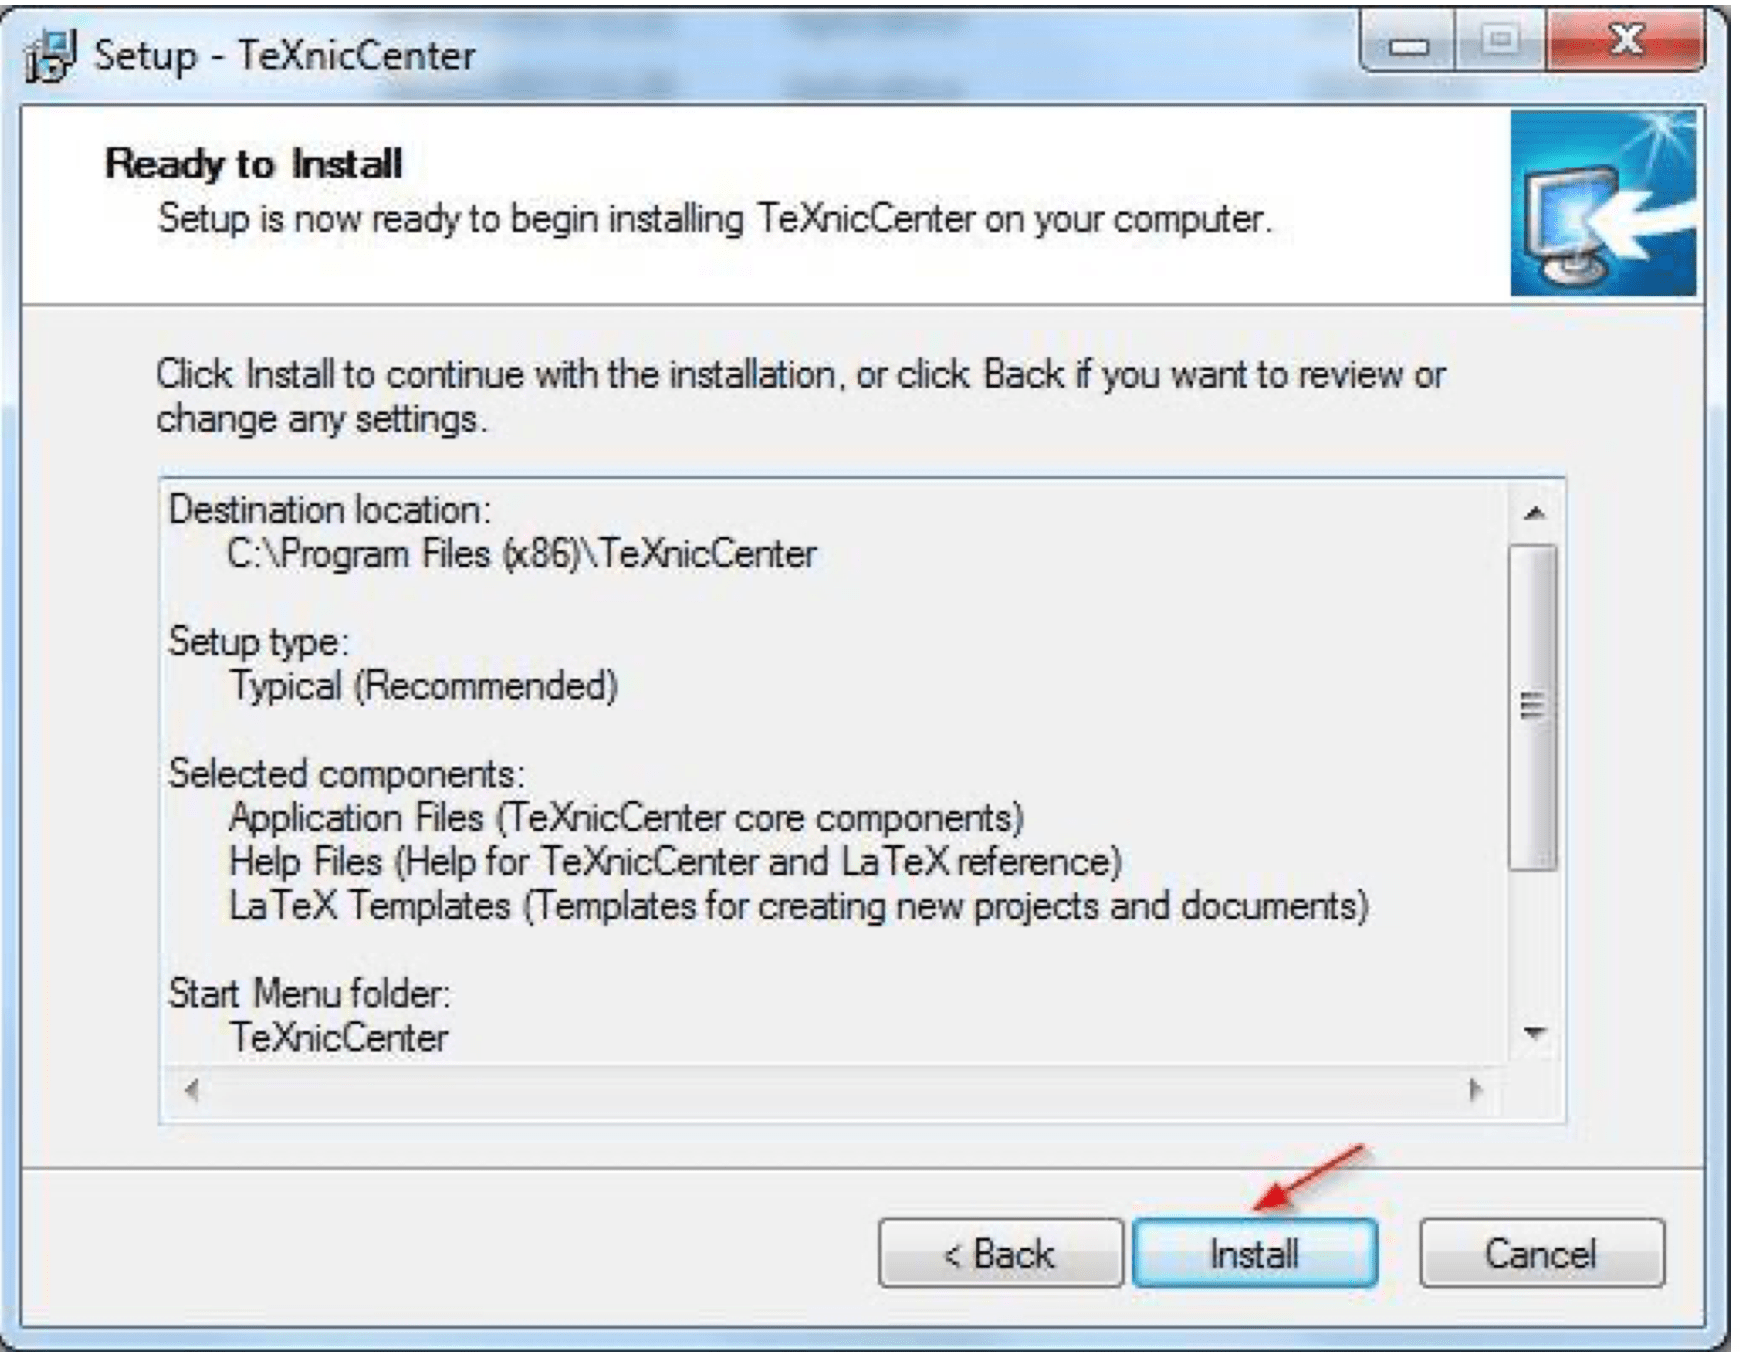
\includegraphics[width=0.6\textwidth]{./fig/texniccenter09}
  \caption{Instalação do TeXnicCenter - Sétima tela.}
  \fontefig{\cite{texnic}}
\end{figure}
\item Apenas aguarde a finalização do processo de instalação.
\begin{figure}[H]
  \centering
  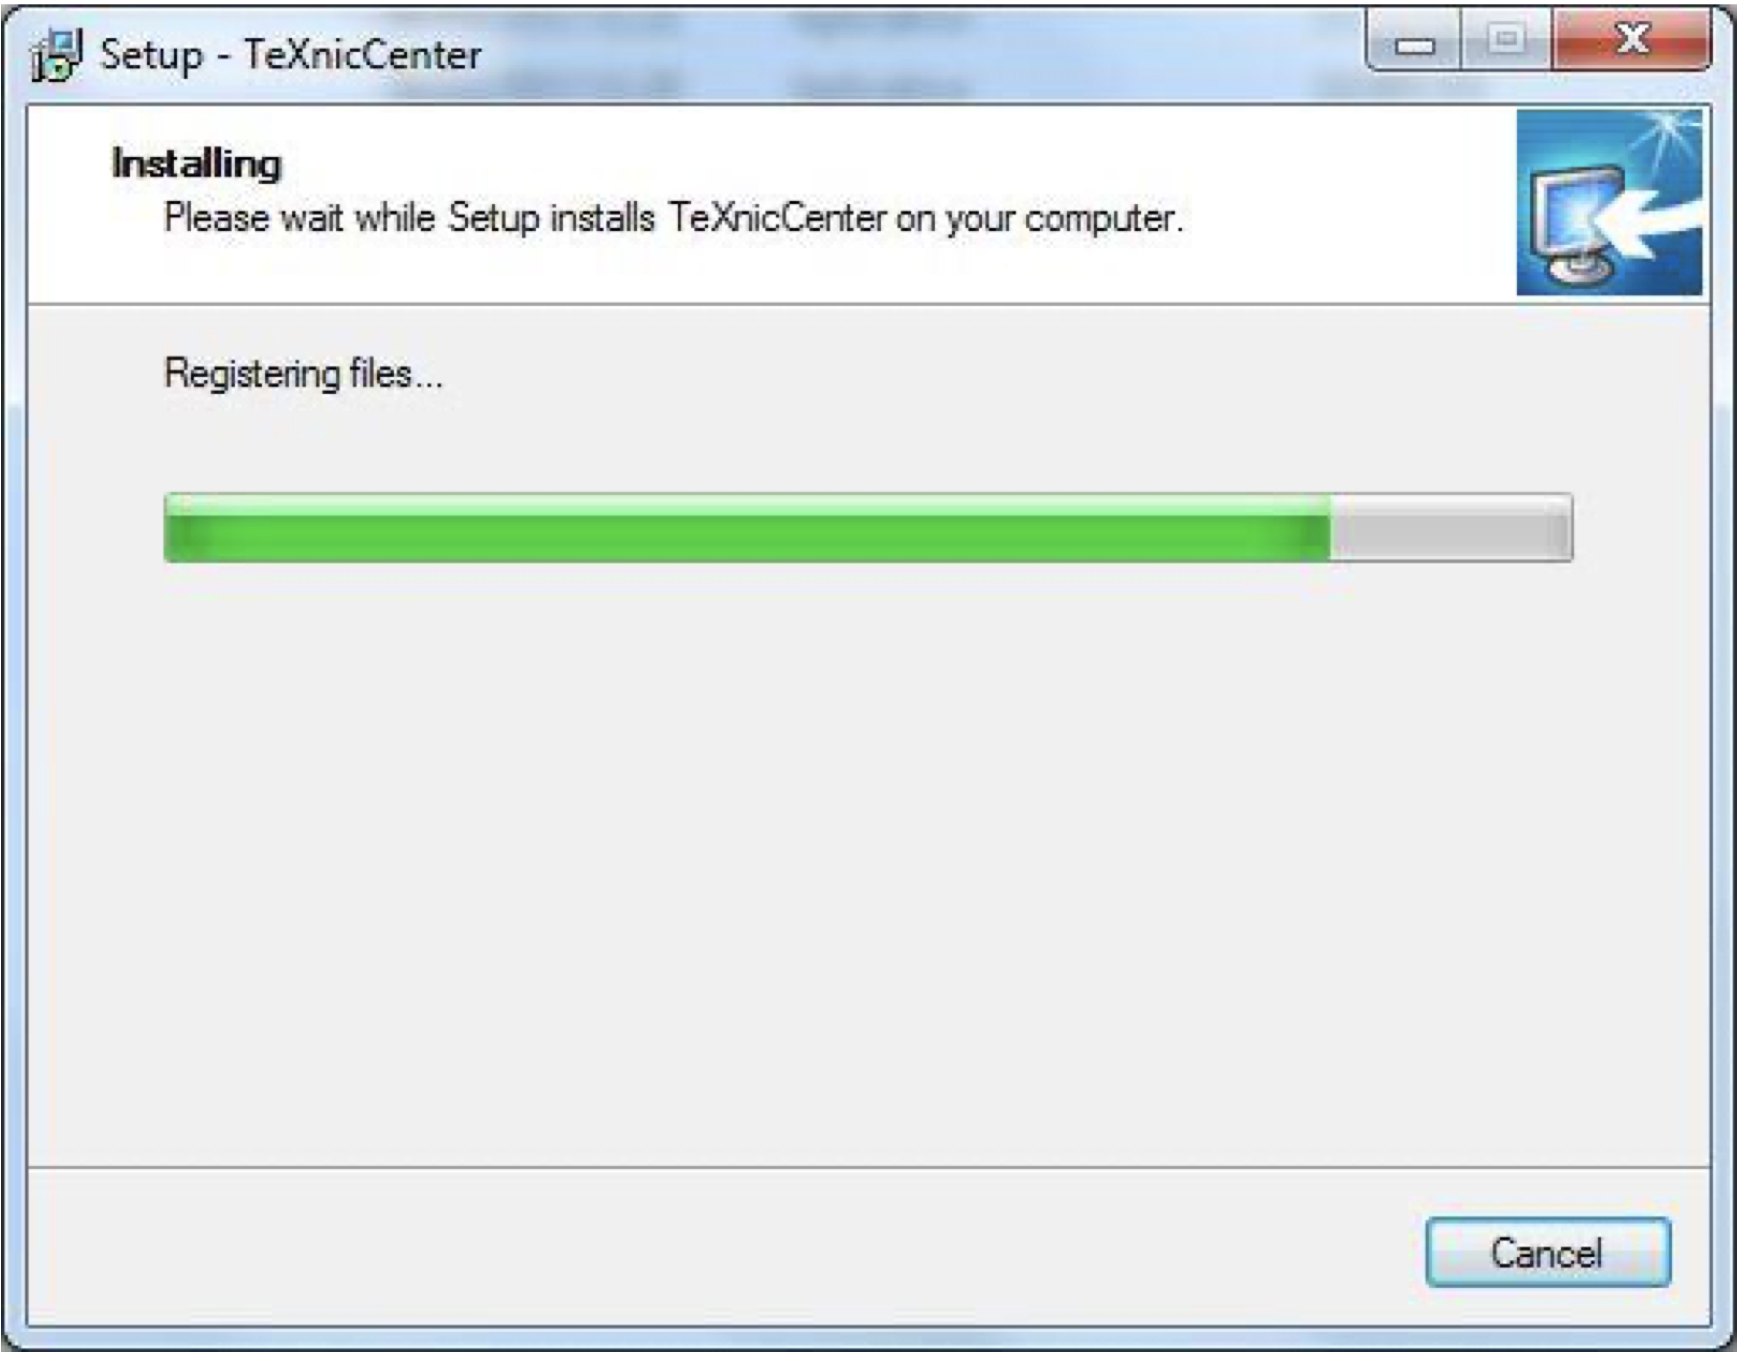
\includegraphics[width=0.6\textwidth]{./fig/texniccenter10}
  \caption{Instalação do TeXnicCenter - Oitava tela.}
  \fontefig{\cite{texnic}}
\end{figure}
\item Para finalizar o processo de instalação clique no botão \textbf{Finish}.
\begin{figure}[H]
  \centering
  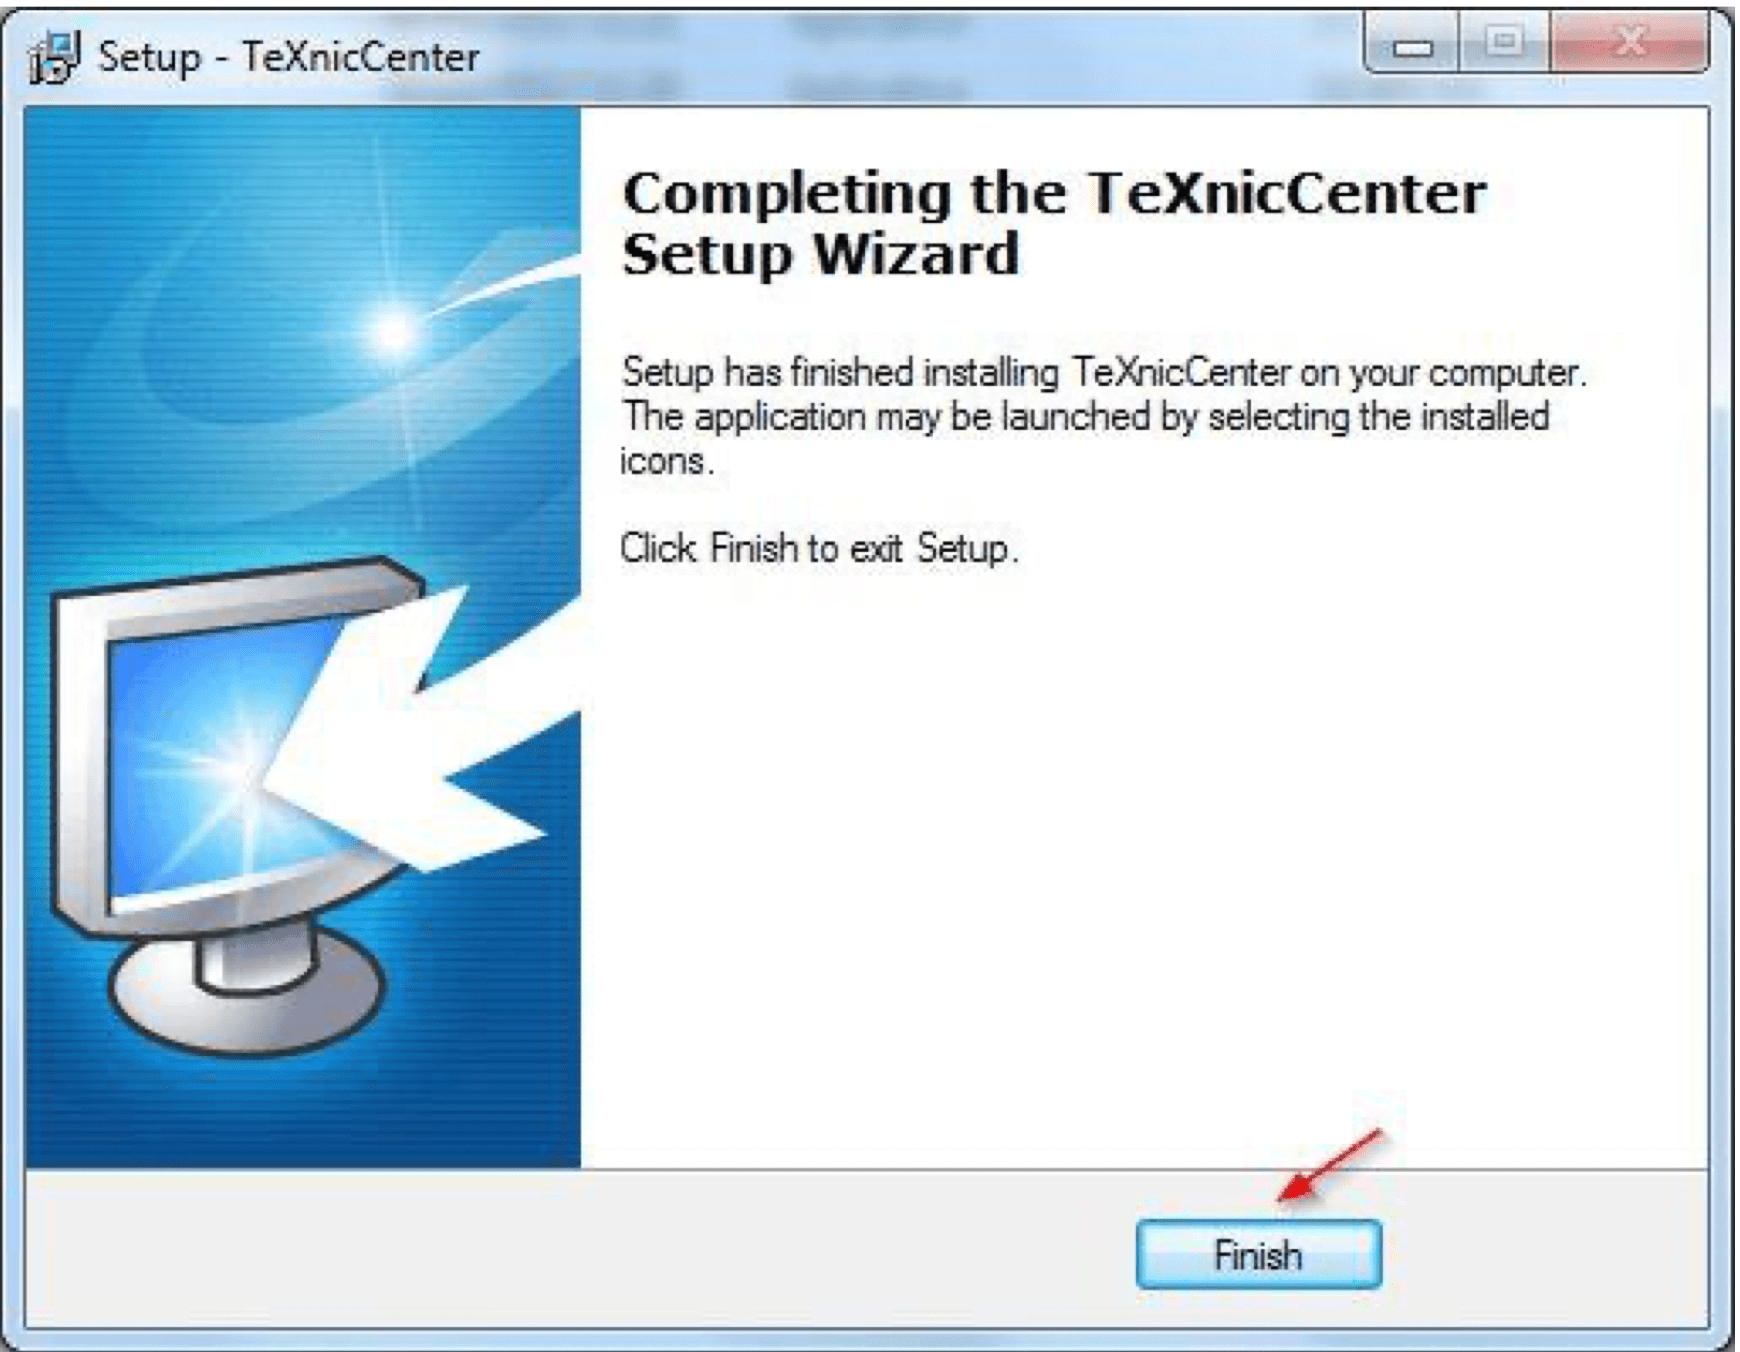
\includegraphics[width=0.6\textwidth]{./fig/texniccenter11}
  \caption{Instalação do TeXnicCenter - Nona tela.}
  \fontefig{\cite{texnic}}
\end{figure}
\end{enumerate}

O TeXnicCenter está instalado em seu computador, agora será necessário configurar o software em sua primeira execução. Os passos a seguir ilustram como deve ser feita a configuração inicial do TeXnicCenter.

\begin{enumerate}
\item Abra o programa TeXnicCenter, ao abrir será exibida uma janela de dicas de uso, clique no botão \textbf{Close} para fechar a janela.
\begin{figure}[H]
  \centering
  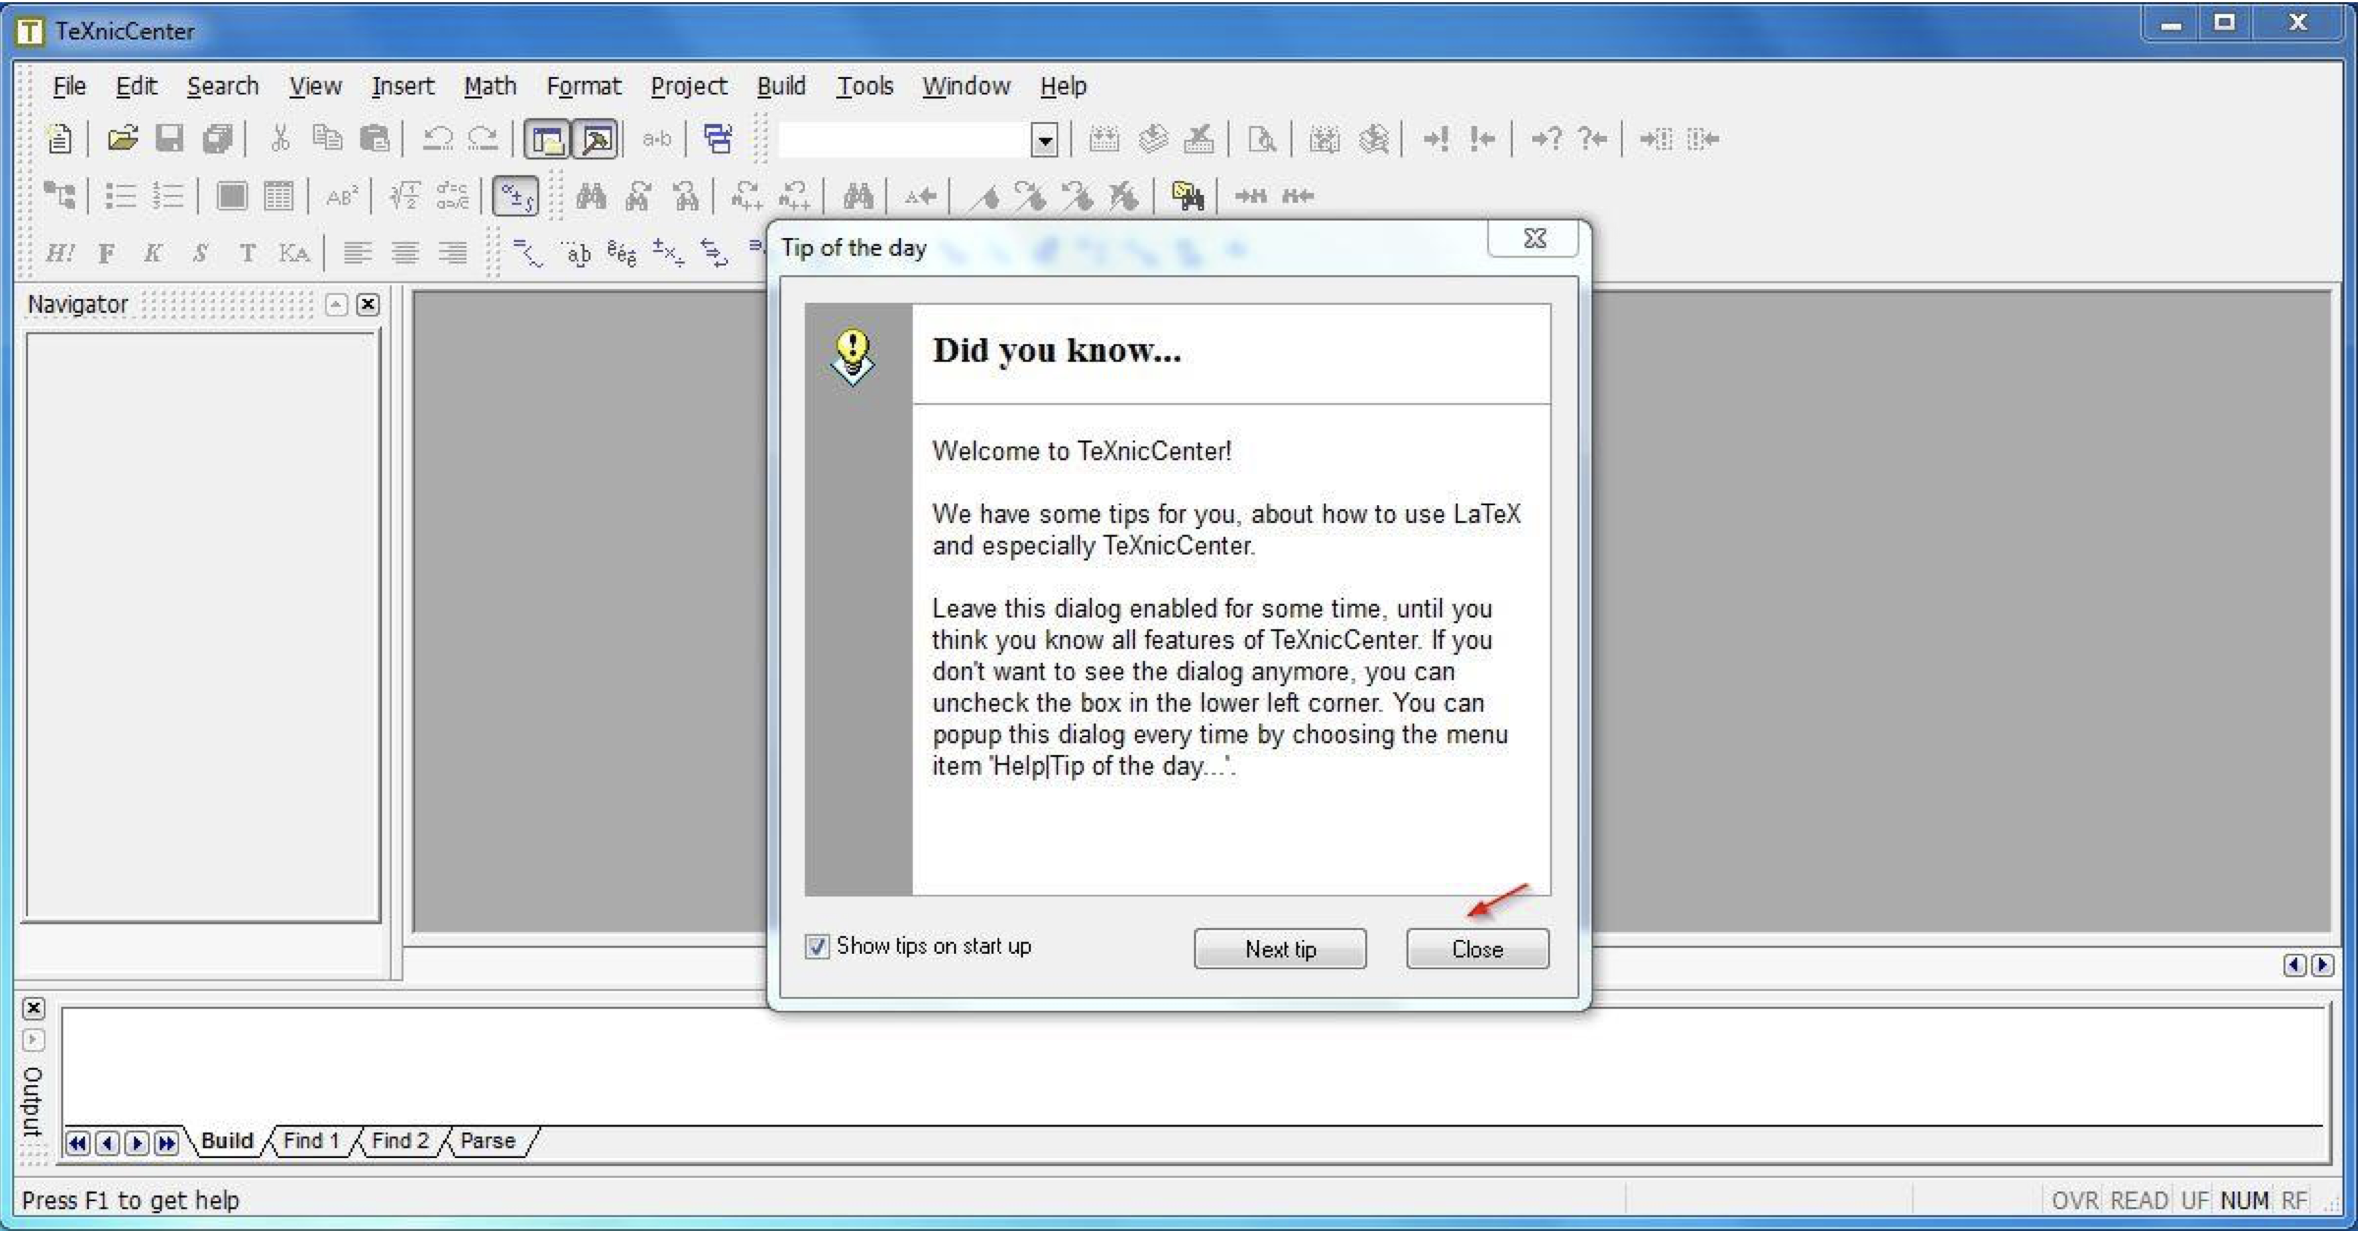
\includegraphics[width=1.0\textwidth]{./fig/texniccenter12}
  \caption{Configuração do TeXnicCenter - Primeira tela.}
  \fontefig{\cite{texnic}}
\end{figure}
\item A janela de configuração inicial do software será exibida clique no botão \textbf{Avançar} para iniciar o processo.
\begin{figure}[H]
  \centering
  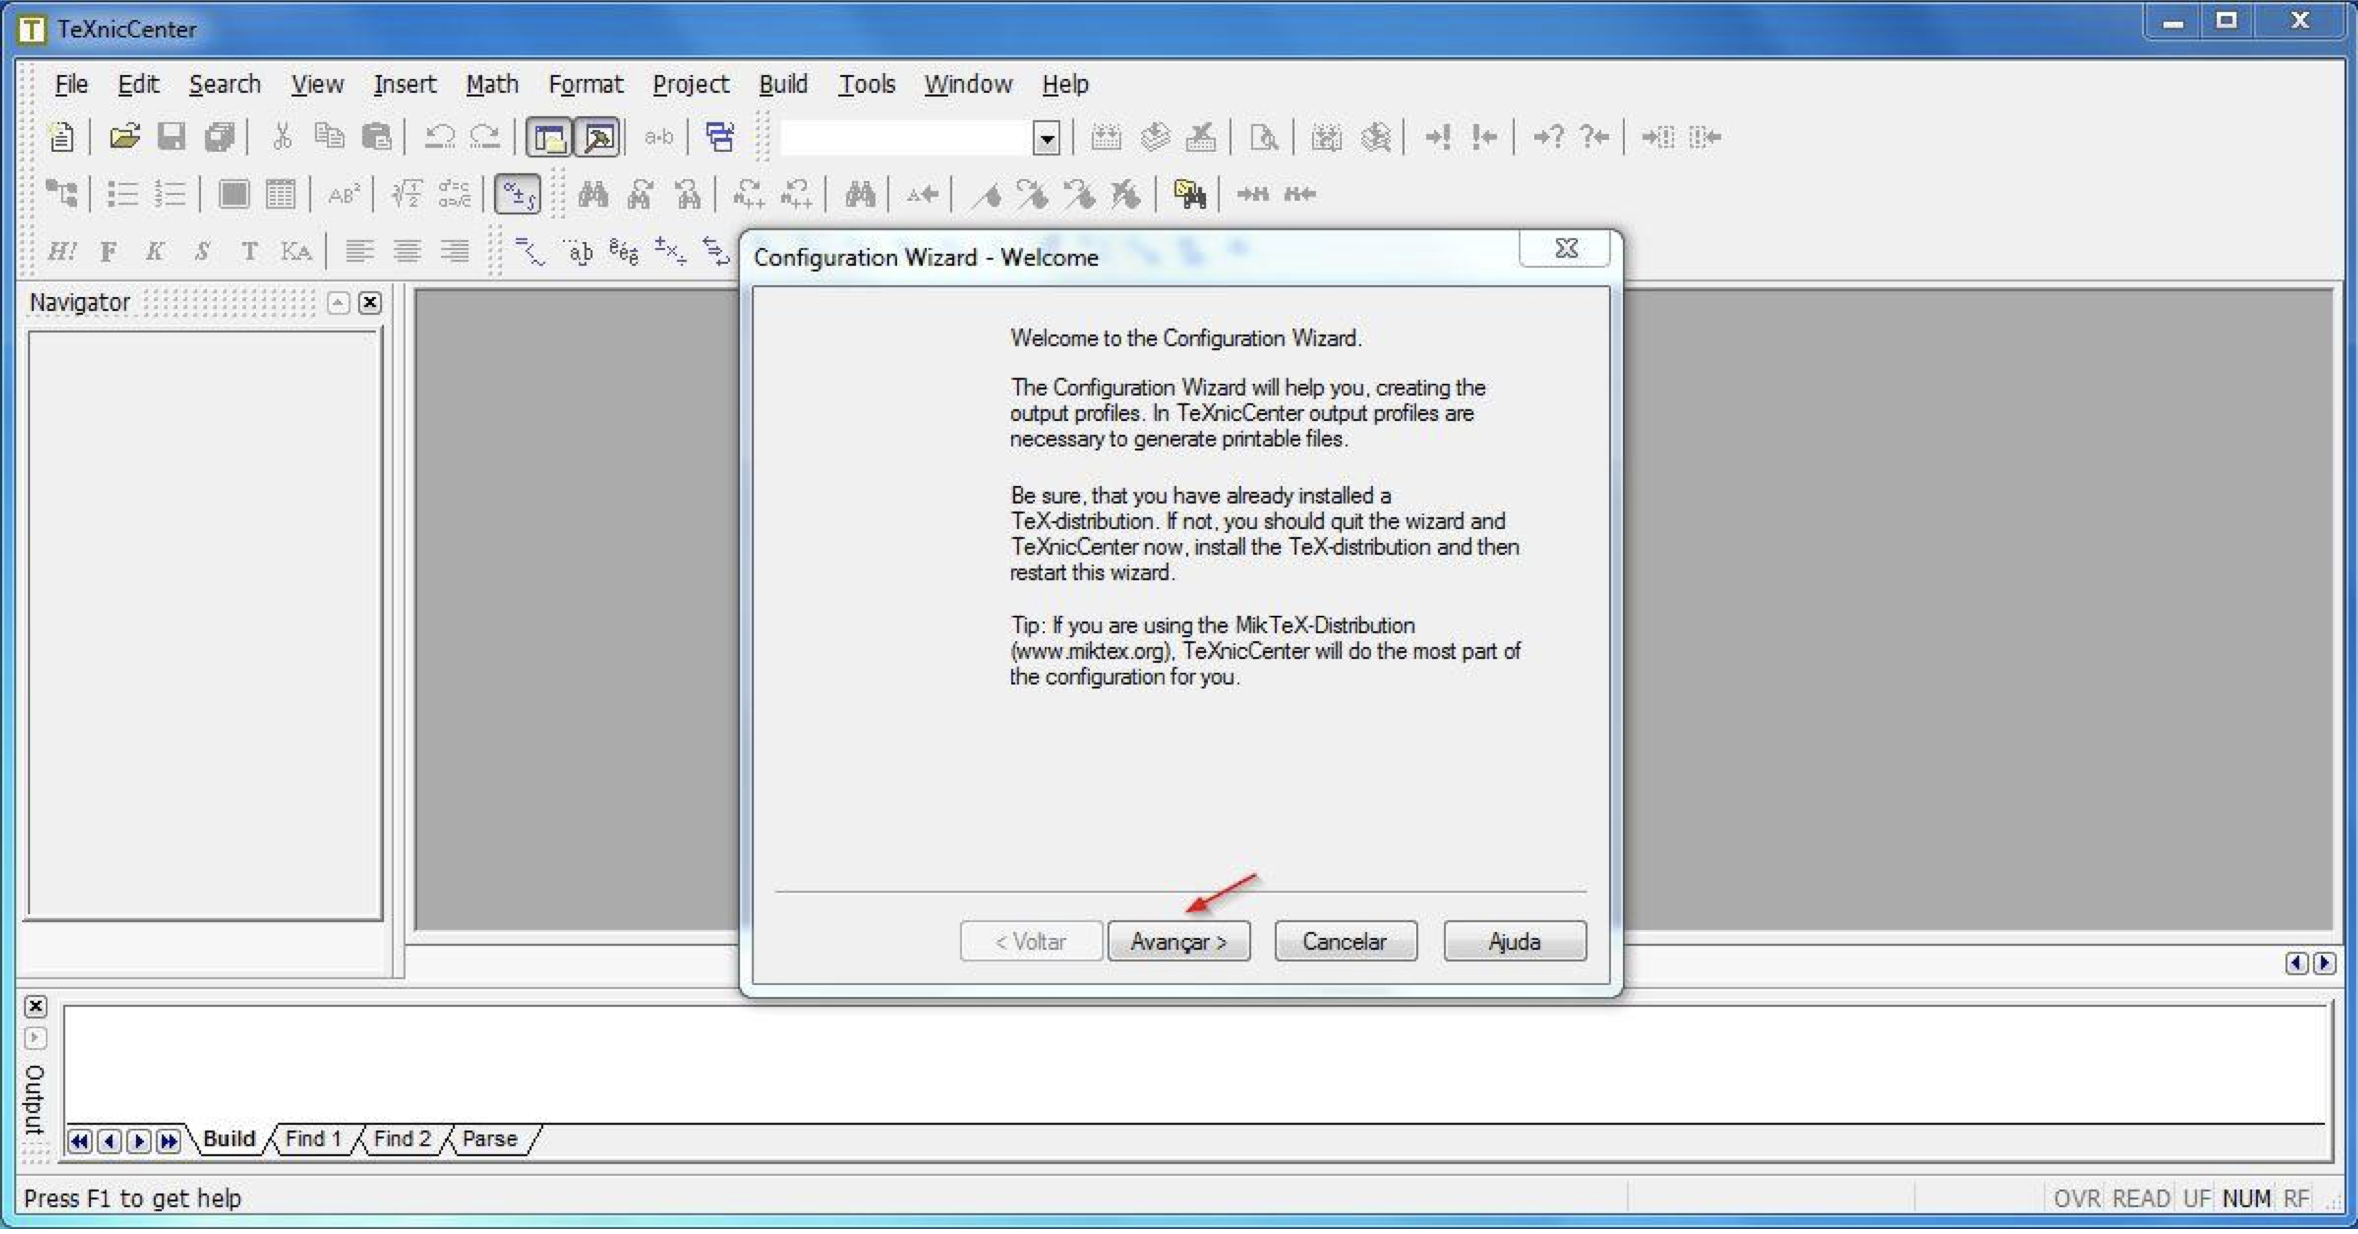
\includegraphics[width=1.0\textwidth]{./fig/texniccenter13}
  \caption{Configuração do TeXnicCenter - Segunda tela.}
  \fontefig{\cite{texnic}}
\end{figure}
\item Na janela exibida será necessário informar na caixa em branco o local onde estão os executáveis do MiKTeX, para isto localize a pasta onde foi instalado o MikTeX (conforme anotado em seu processo de instalação, neste tutorial é a pasta: \aspas{C:$\backslash$Program Files (x86)$\backslash$MiKTeX 2.9}, mas pode variar dependendo da versão do Windows utilizado), dentro da pasta do MikTeX localize a pasta \textbf{miktex} e dentro dela a pasta \textbf{bin}.
\begin{figure}[H]
  \centering
  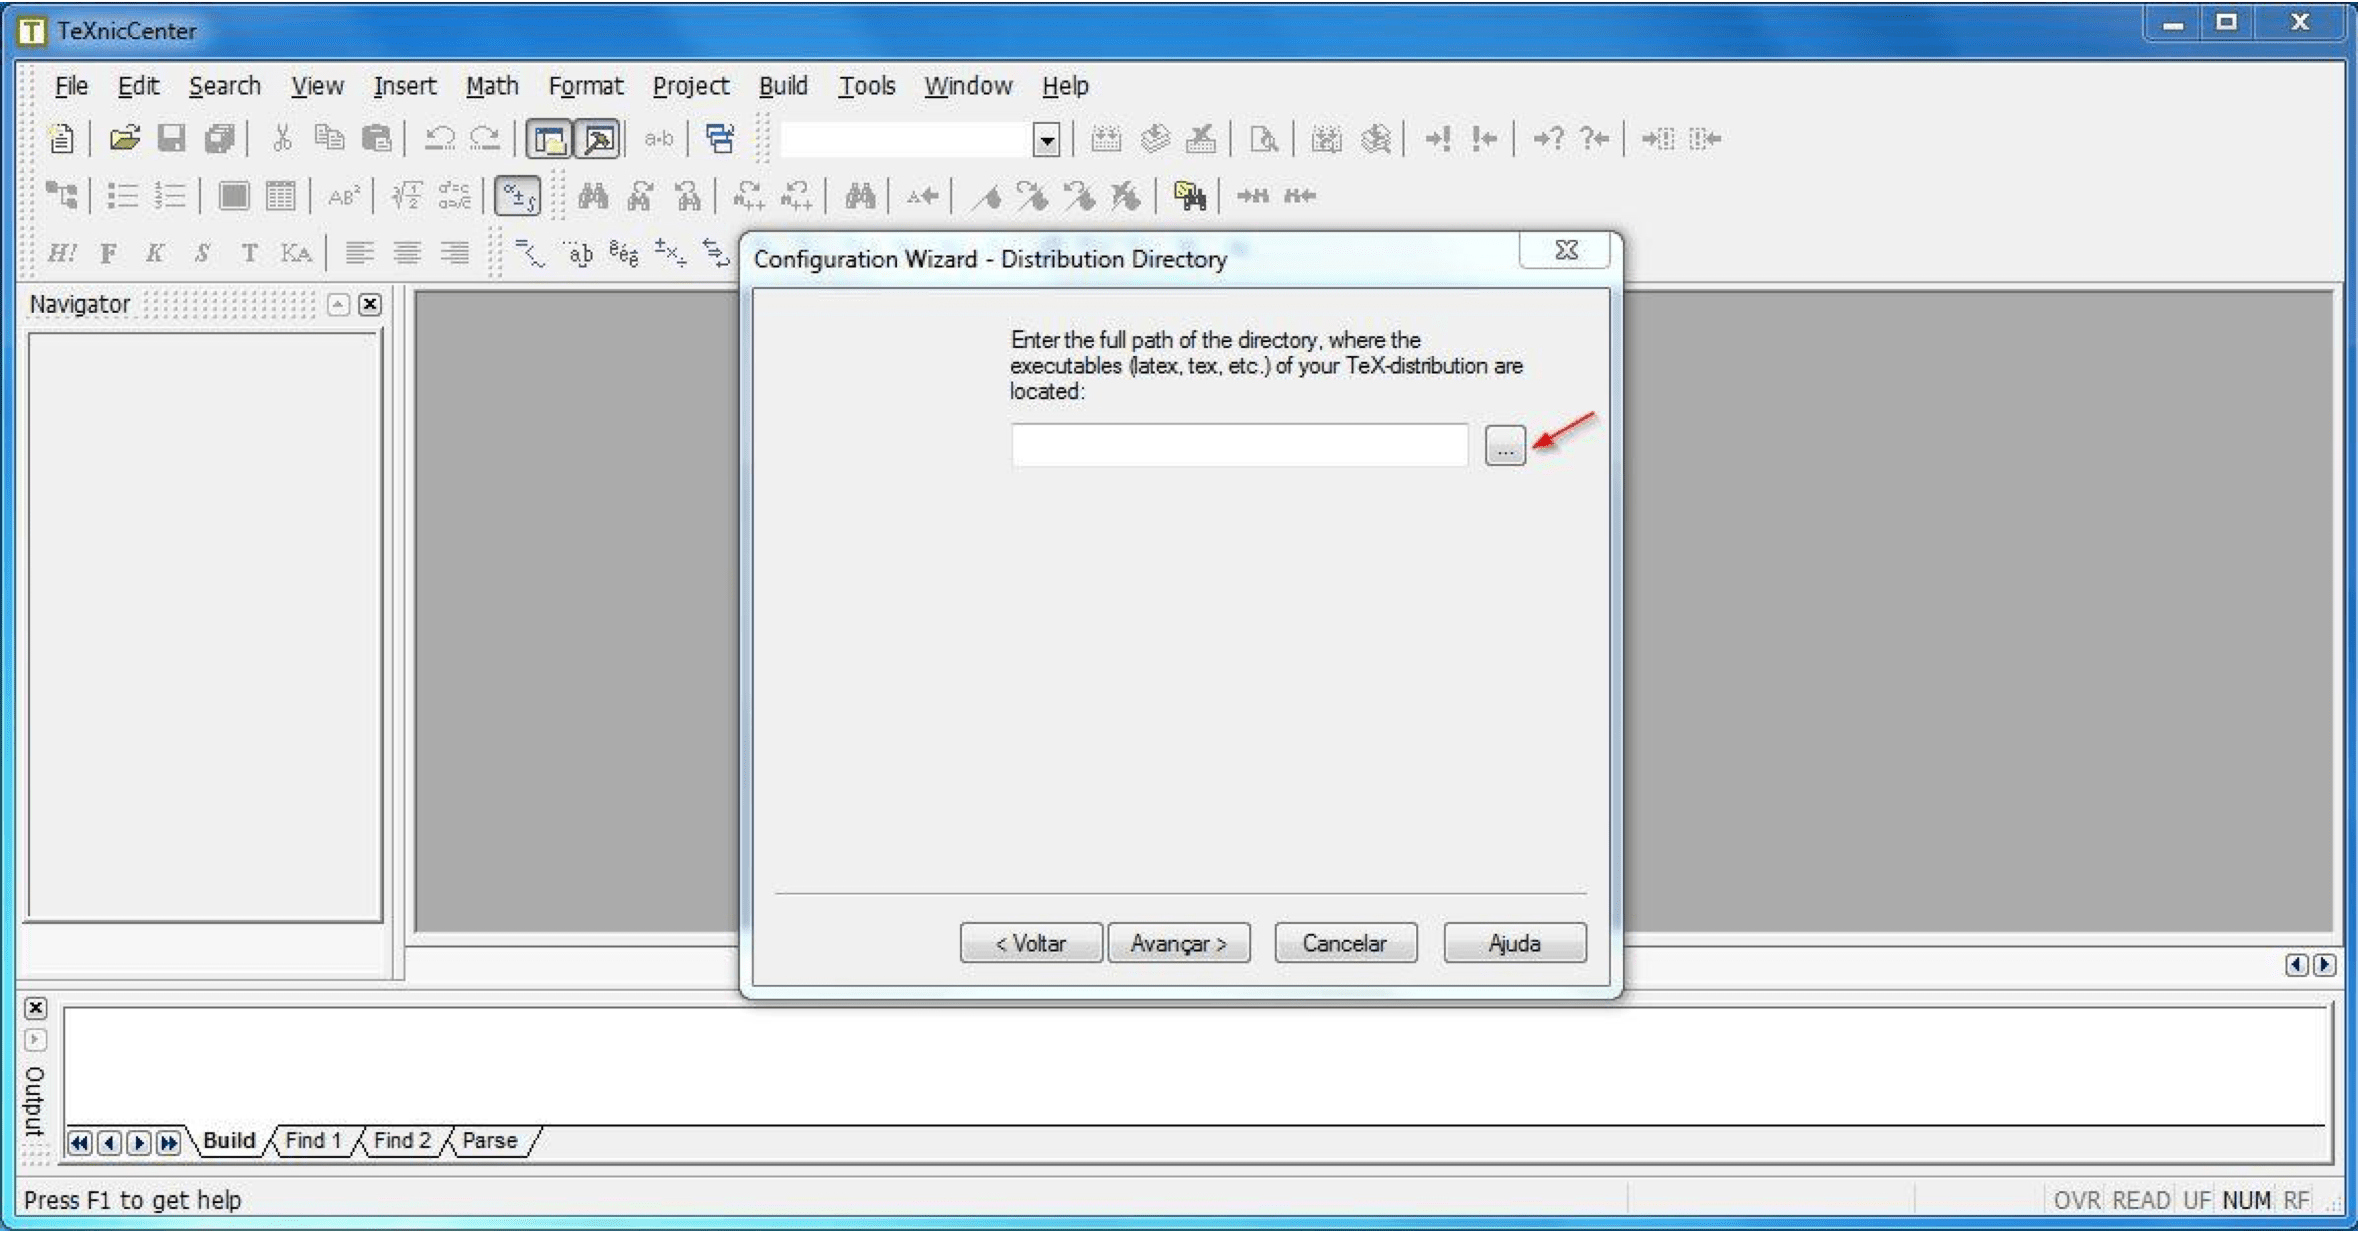
\includegraphics[width=1.0\textwidth]{./fig/texniccenter14}
  \caption{Configuração do TeXnicCenter - Terceira tela.}
  \fontefig{\cite{texnic}}
\end{figure}
Você pode copiar e colar o local dos executáveis do MiKTeX (neste tutorial é: \aspas{C:$\backslash$Program Files (x86)$\backslash$MiKTeX 2. 9$\backslash$miktex$\backslash$bin}, mas pode variar dependendo da versão do Windows utilizado) na caixa em branco ou pode procurar a pasta utilizando o botão \aspas{...}.
\item Após selecionada a pasta dos executáveis do MiKTeX, clique no botão \textbf{Avançar}.
\begin{figure}[H]
  \centering
  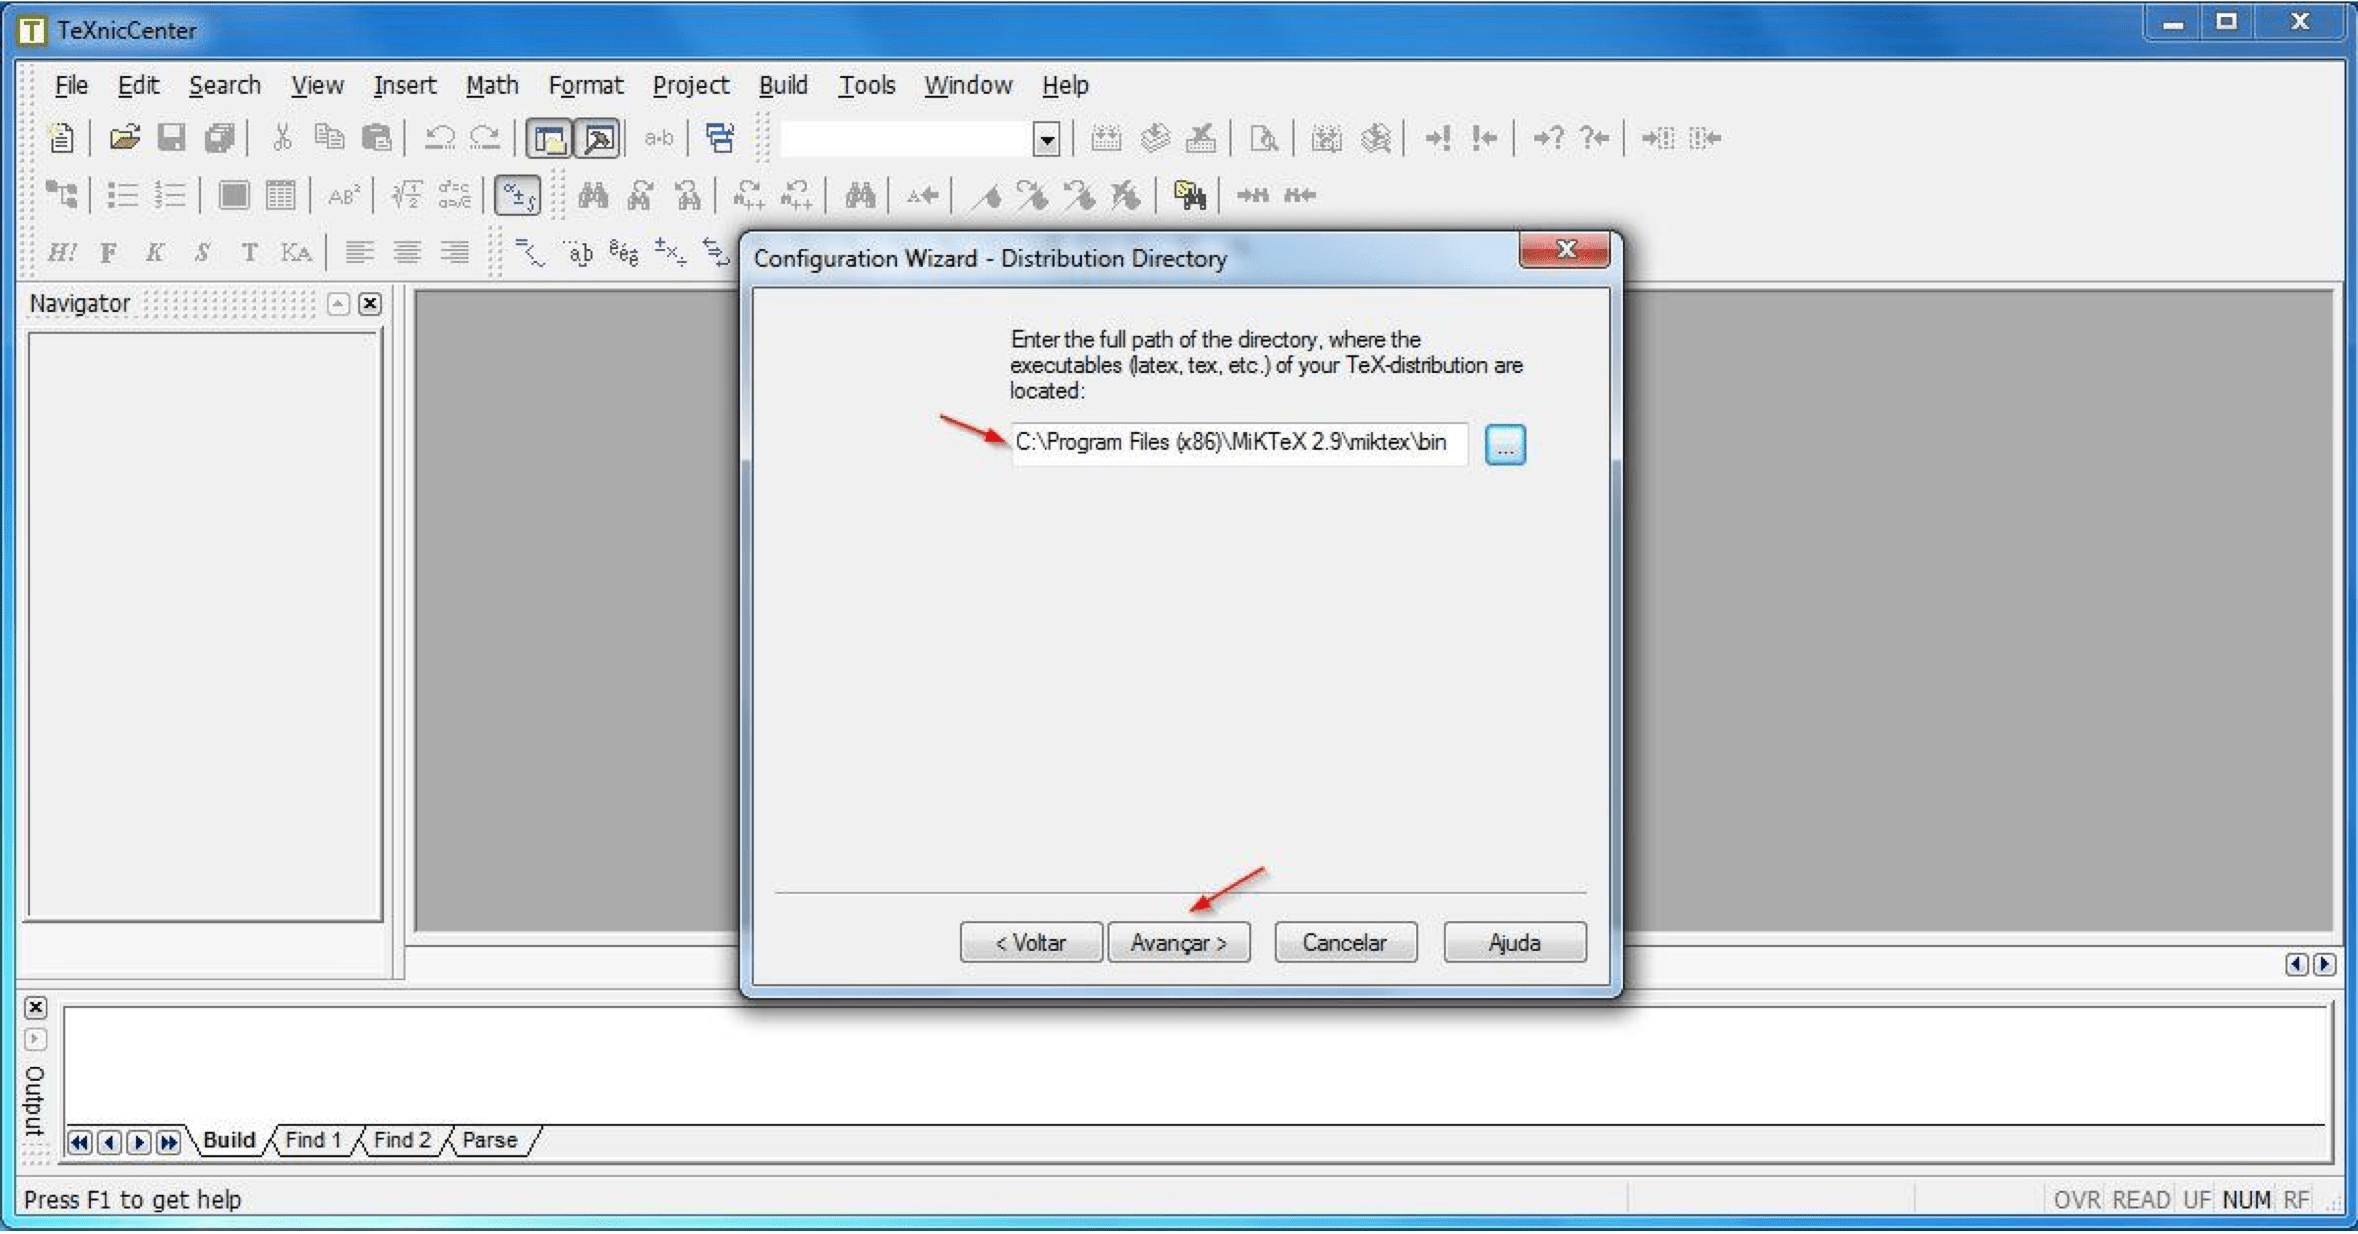
\includegraphics[width=1.0\textwidth]{./fig/texniccenter15}
  \caption{Configuração do TeXnicCenter - Quarta tela.}
  \fontefig{\cite{texnic}}
\end{figure}
\item Serão exibidas as opções para configuração do PostScript que são opcionais, clique apenas no botão \textbf{Avançar}.
\begin{figure}[H]
  \centering
  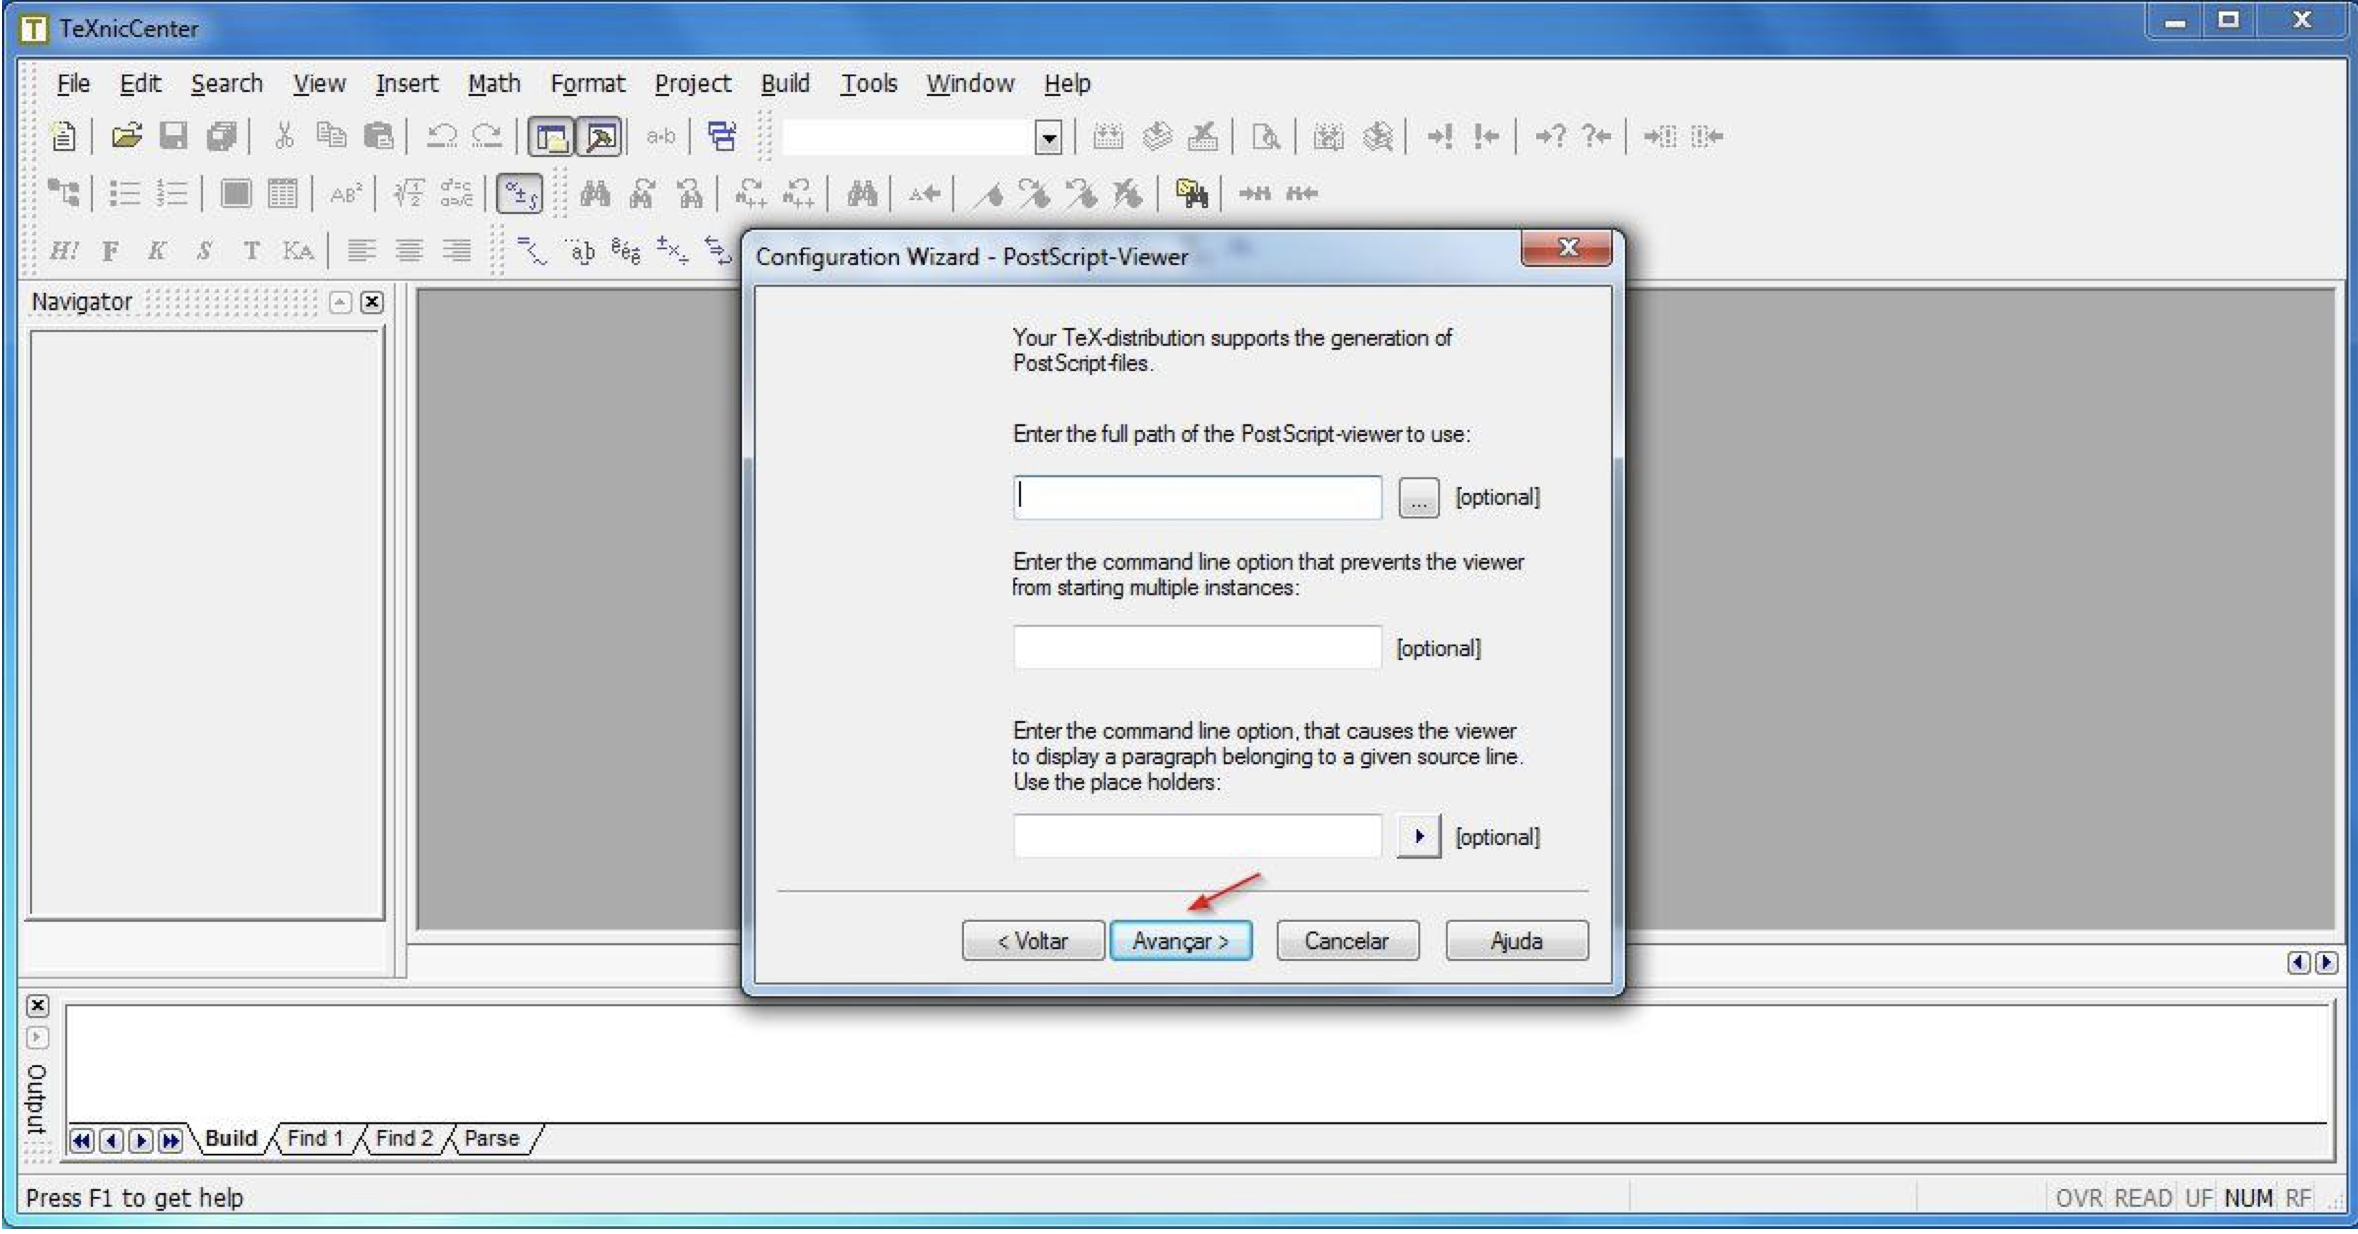
\includegraphics[width=1.0\textwidth]{./fig/texniccenter16}
  \caption{Configuração do TeXnicCenter - Quinta tela.}
  \fontefig{\cite{texnic}}
\end{figure}
\item Agora serão exibidas as opções de PDF opcionais, apenas clique no botão \textbf{Avançar}.
\begin{figure}[H]
  \centering
  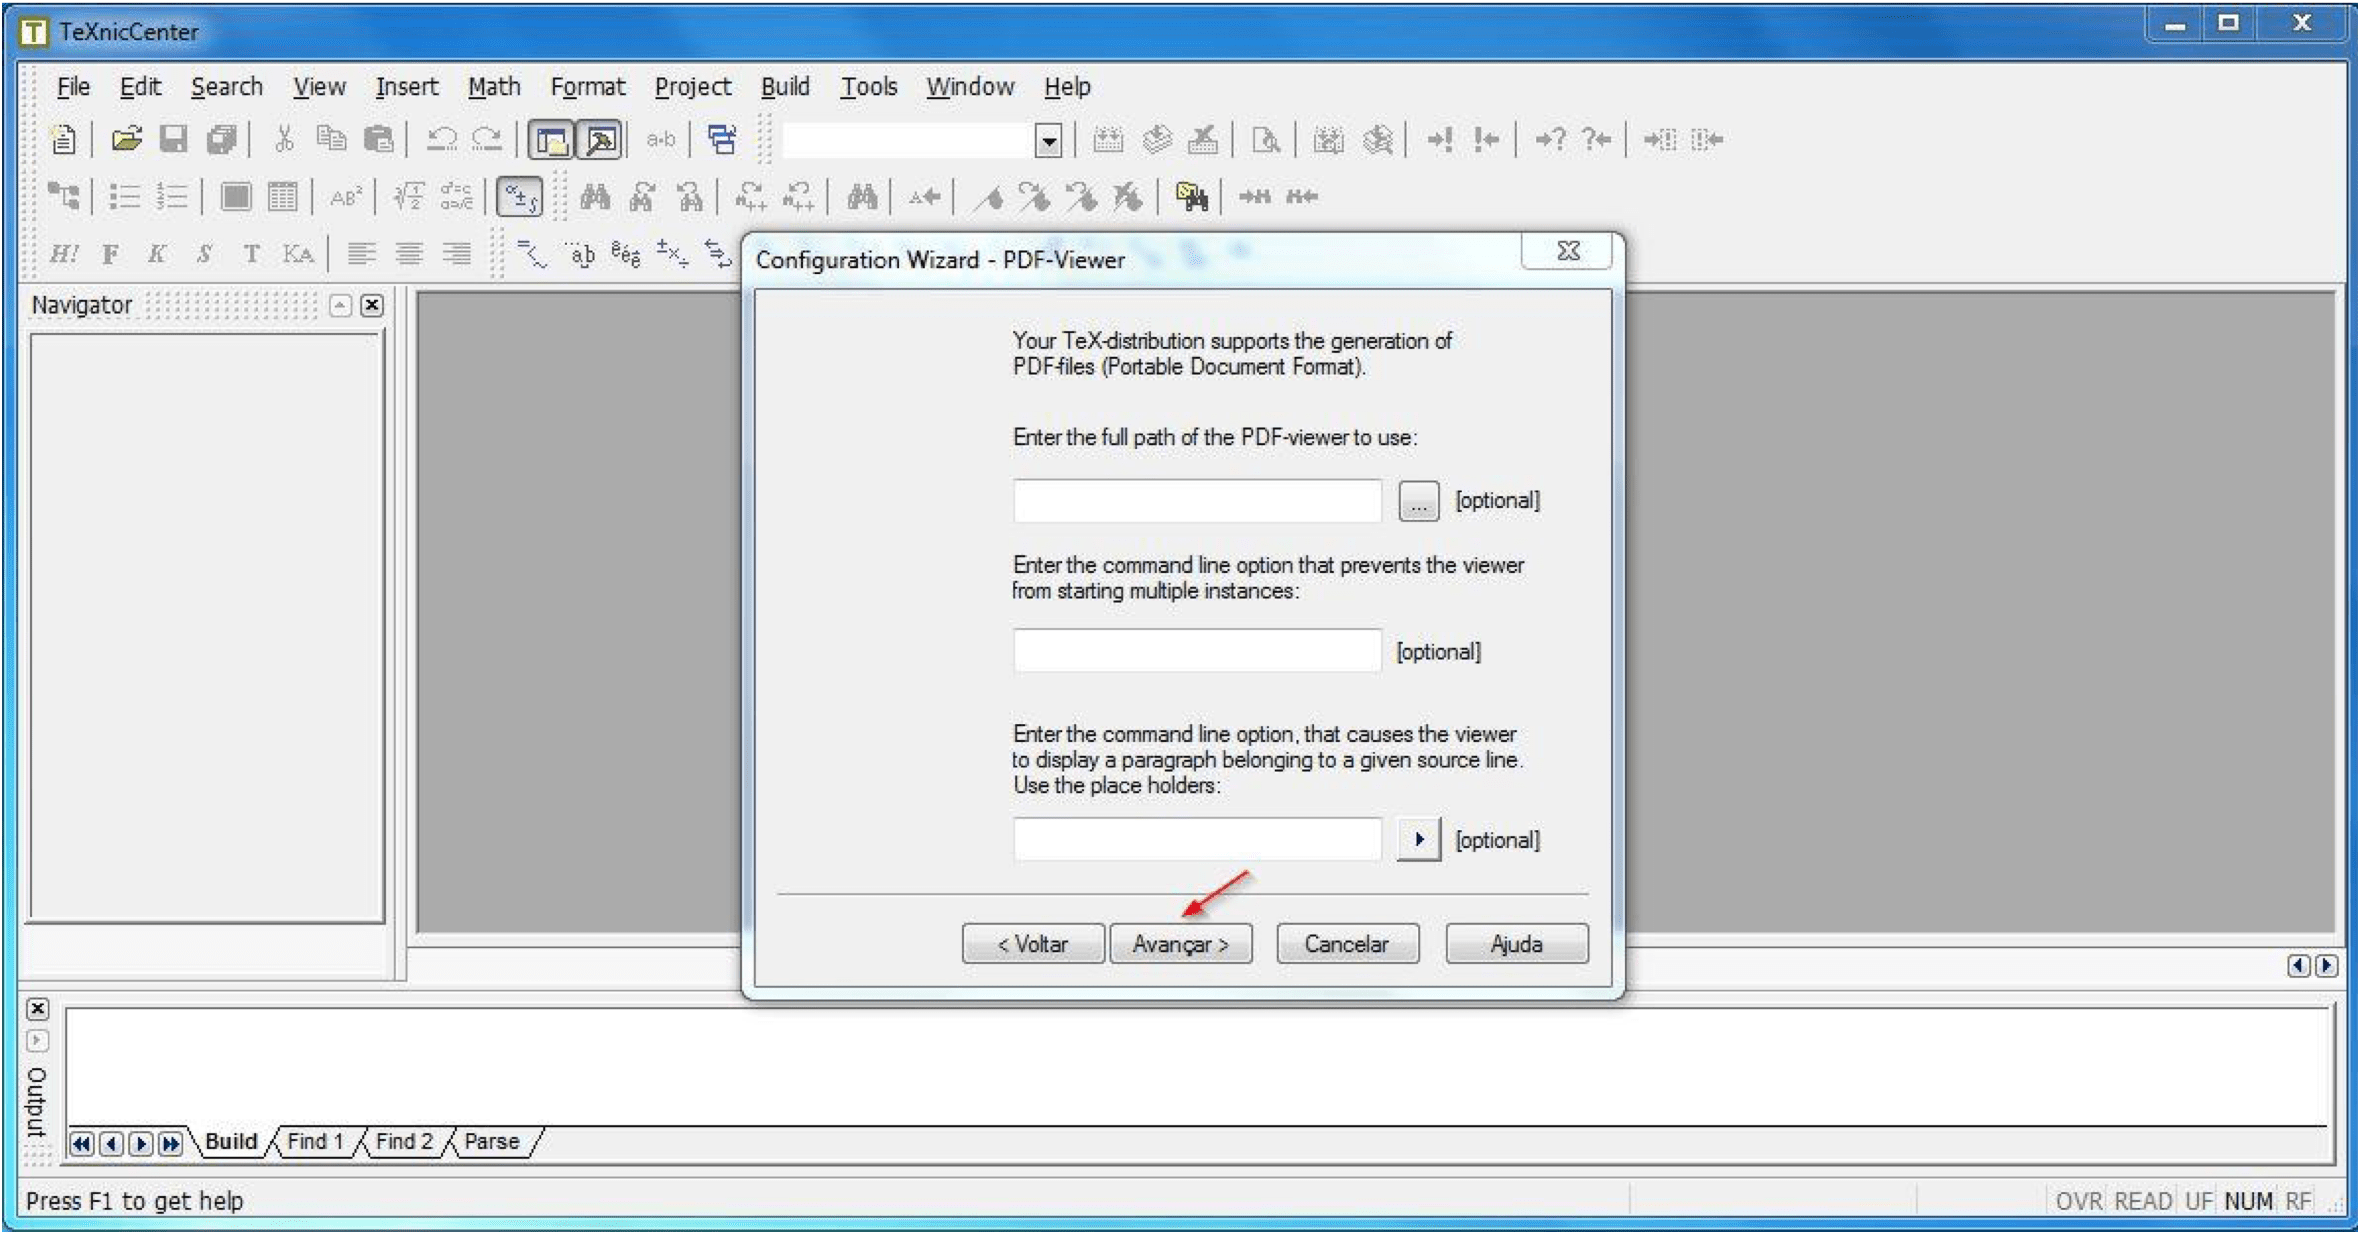
\includegraphics[width=1.0\textwidth]{./fig/texniccenter17}
  \caption{Configuração do TeXnicCenter - Sexta tela.}
  \fontefig{\cite{texnic}}
\end{figure}
\item Serão exibidos os nomes das configurações que serão feitas, apenas clique no botão \textbf{Concluir} para finalizar a configuração.
\begin{figure}[H]
  \centering
  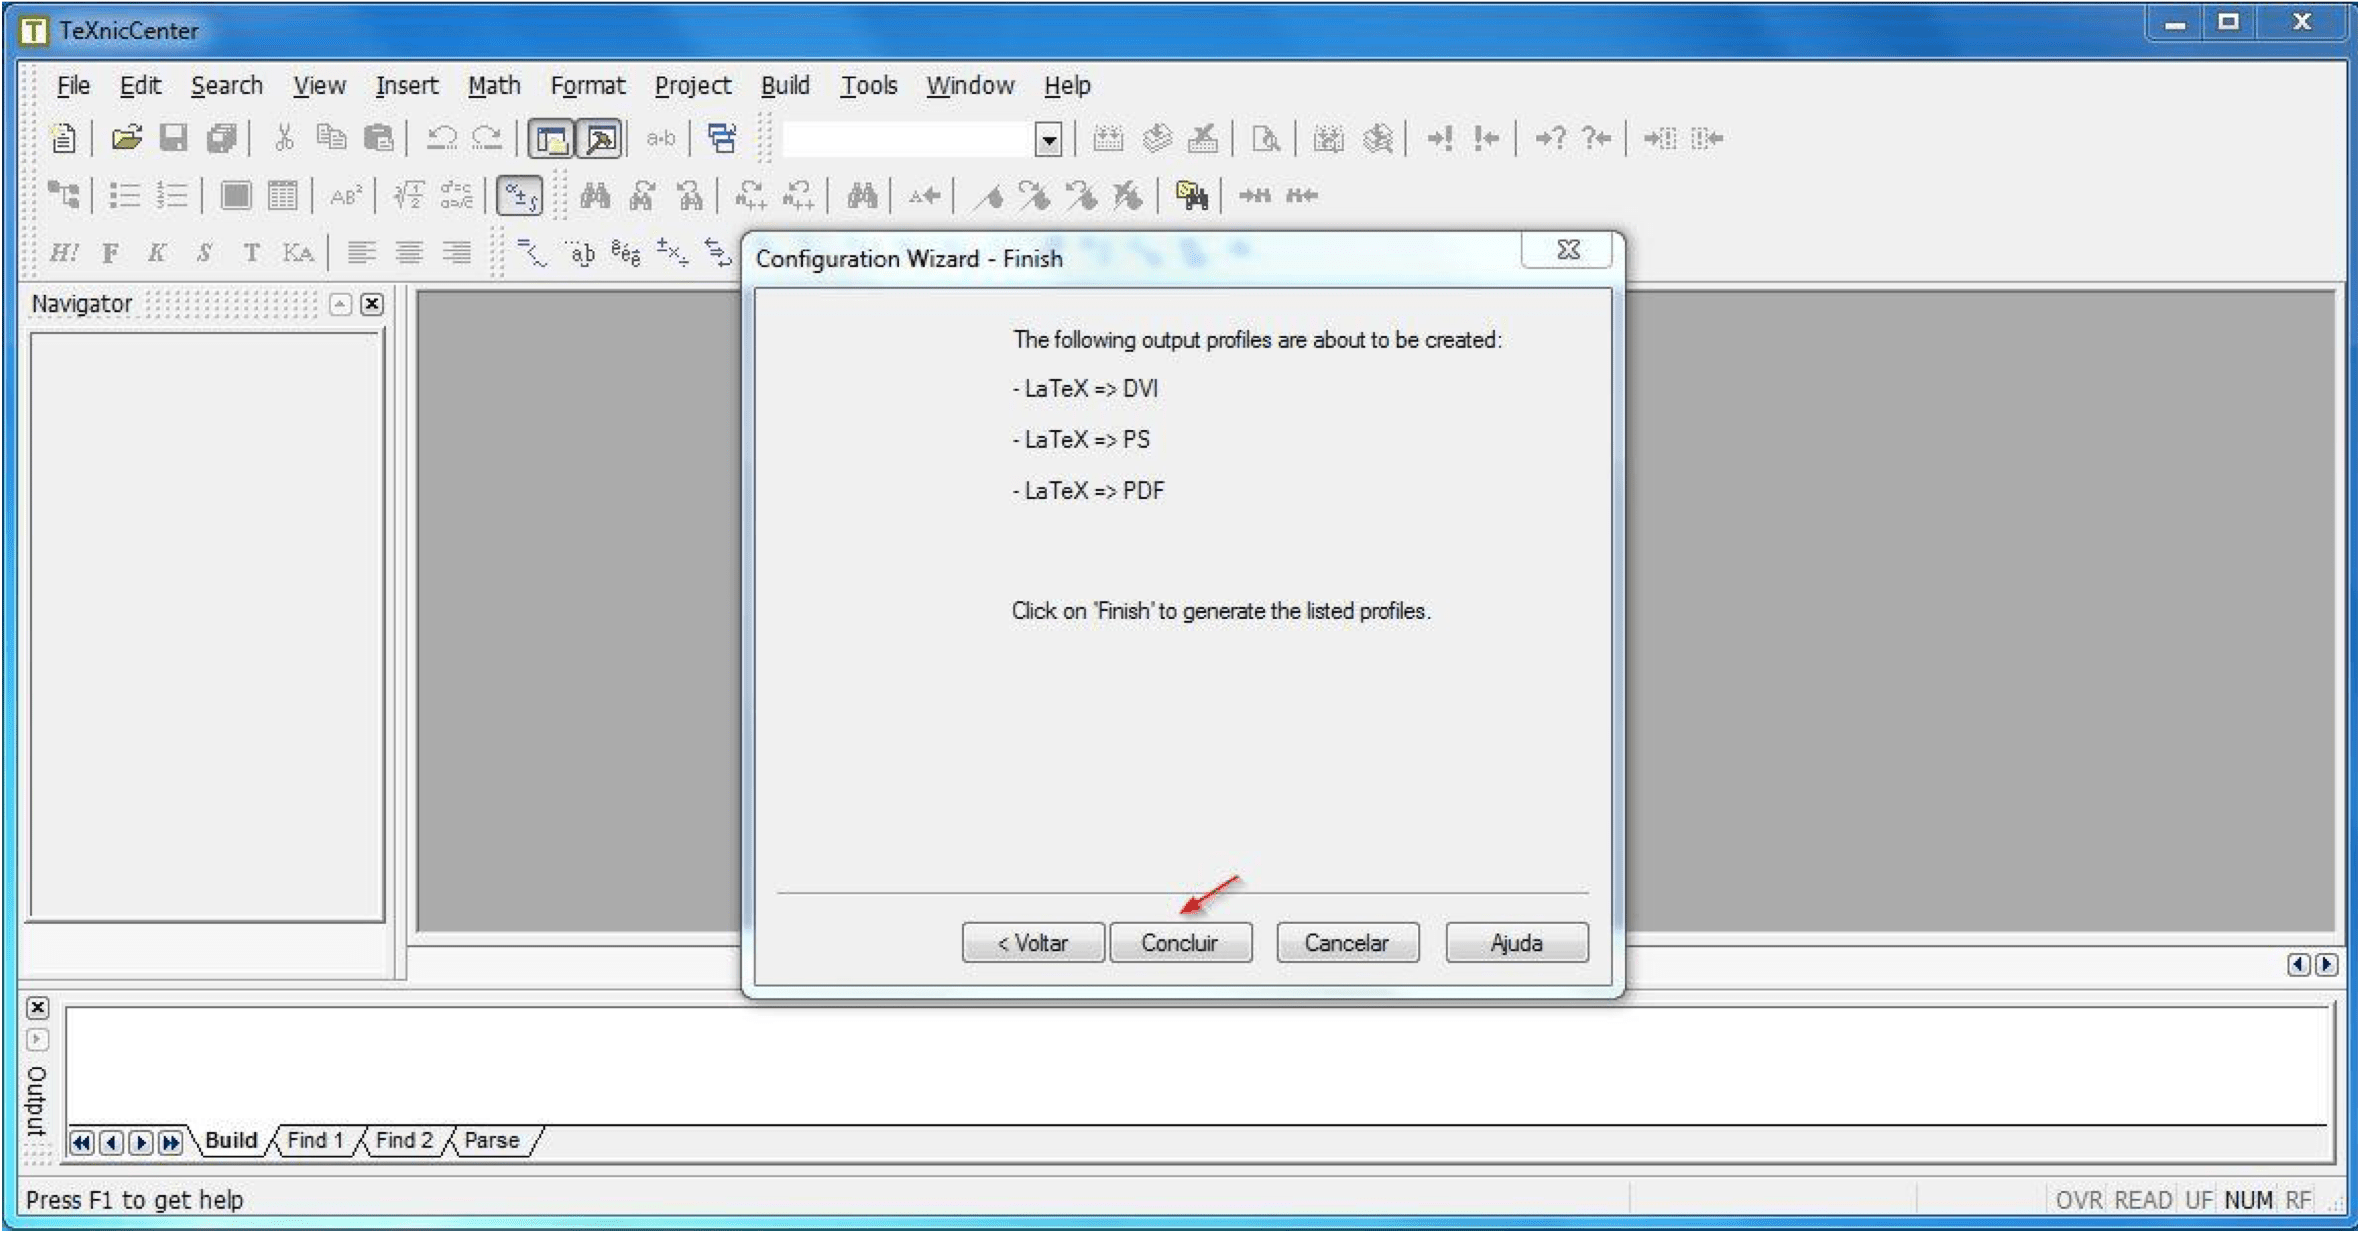
\includegraphics[width=1.0\textwidth]{./fig/texniccenter18}
  \caption{Configuração do TeXnicCenter - Sétima tela.}
  \fontefig{\cite{texnic}}
\end{figure}
\end{enumerate}

\section{Instalando o corretor ortográfico}

Por padrão o TeXnicCenter não vem com corretor ortográfico para português. Para instalá-lo siga os passos a seguir \cite{texnic}.

\begin{enumerate}
\item Faça o download do verificador ortográfico em \url{https://pt-br.libreoffice.org/projetos/vero/}.
\begin{figure}[H]
  \centering
  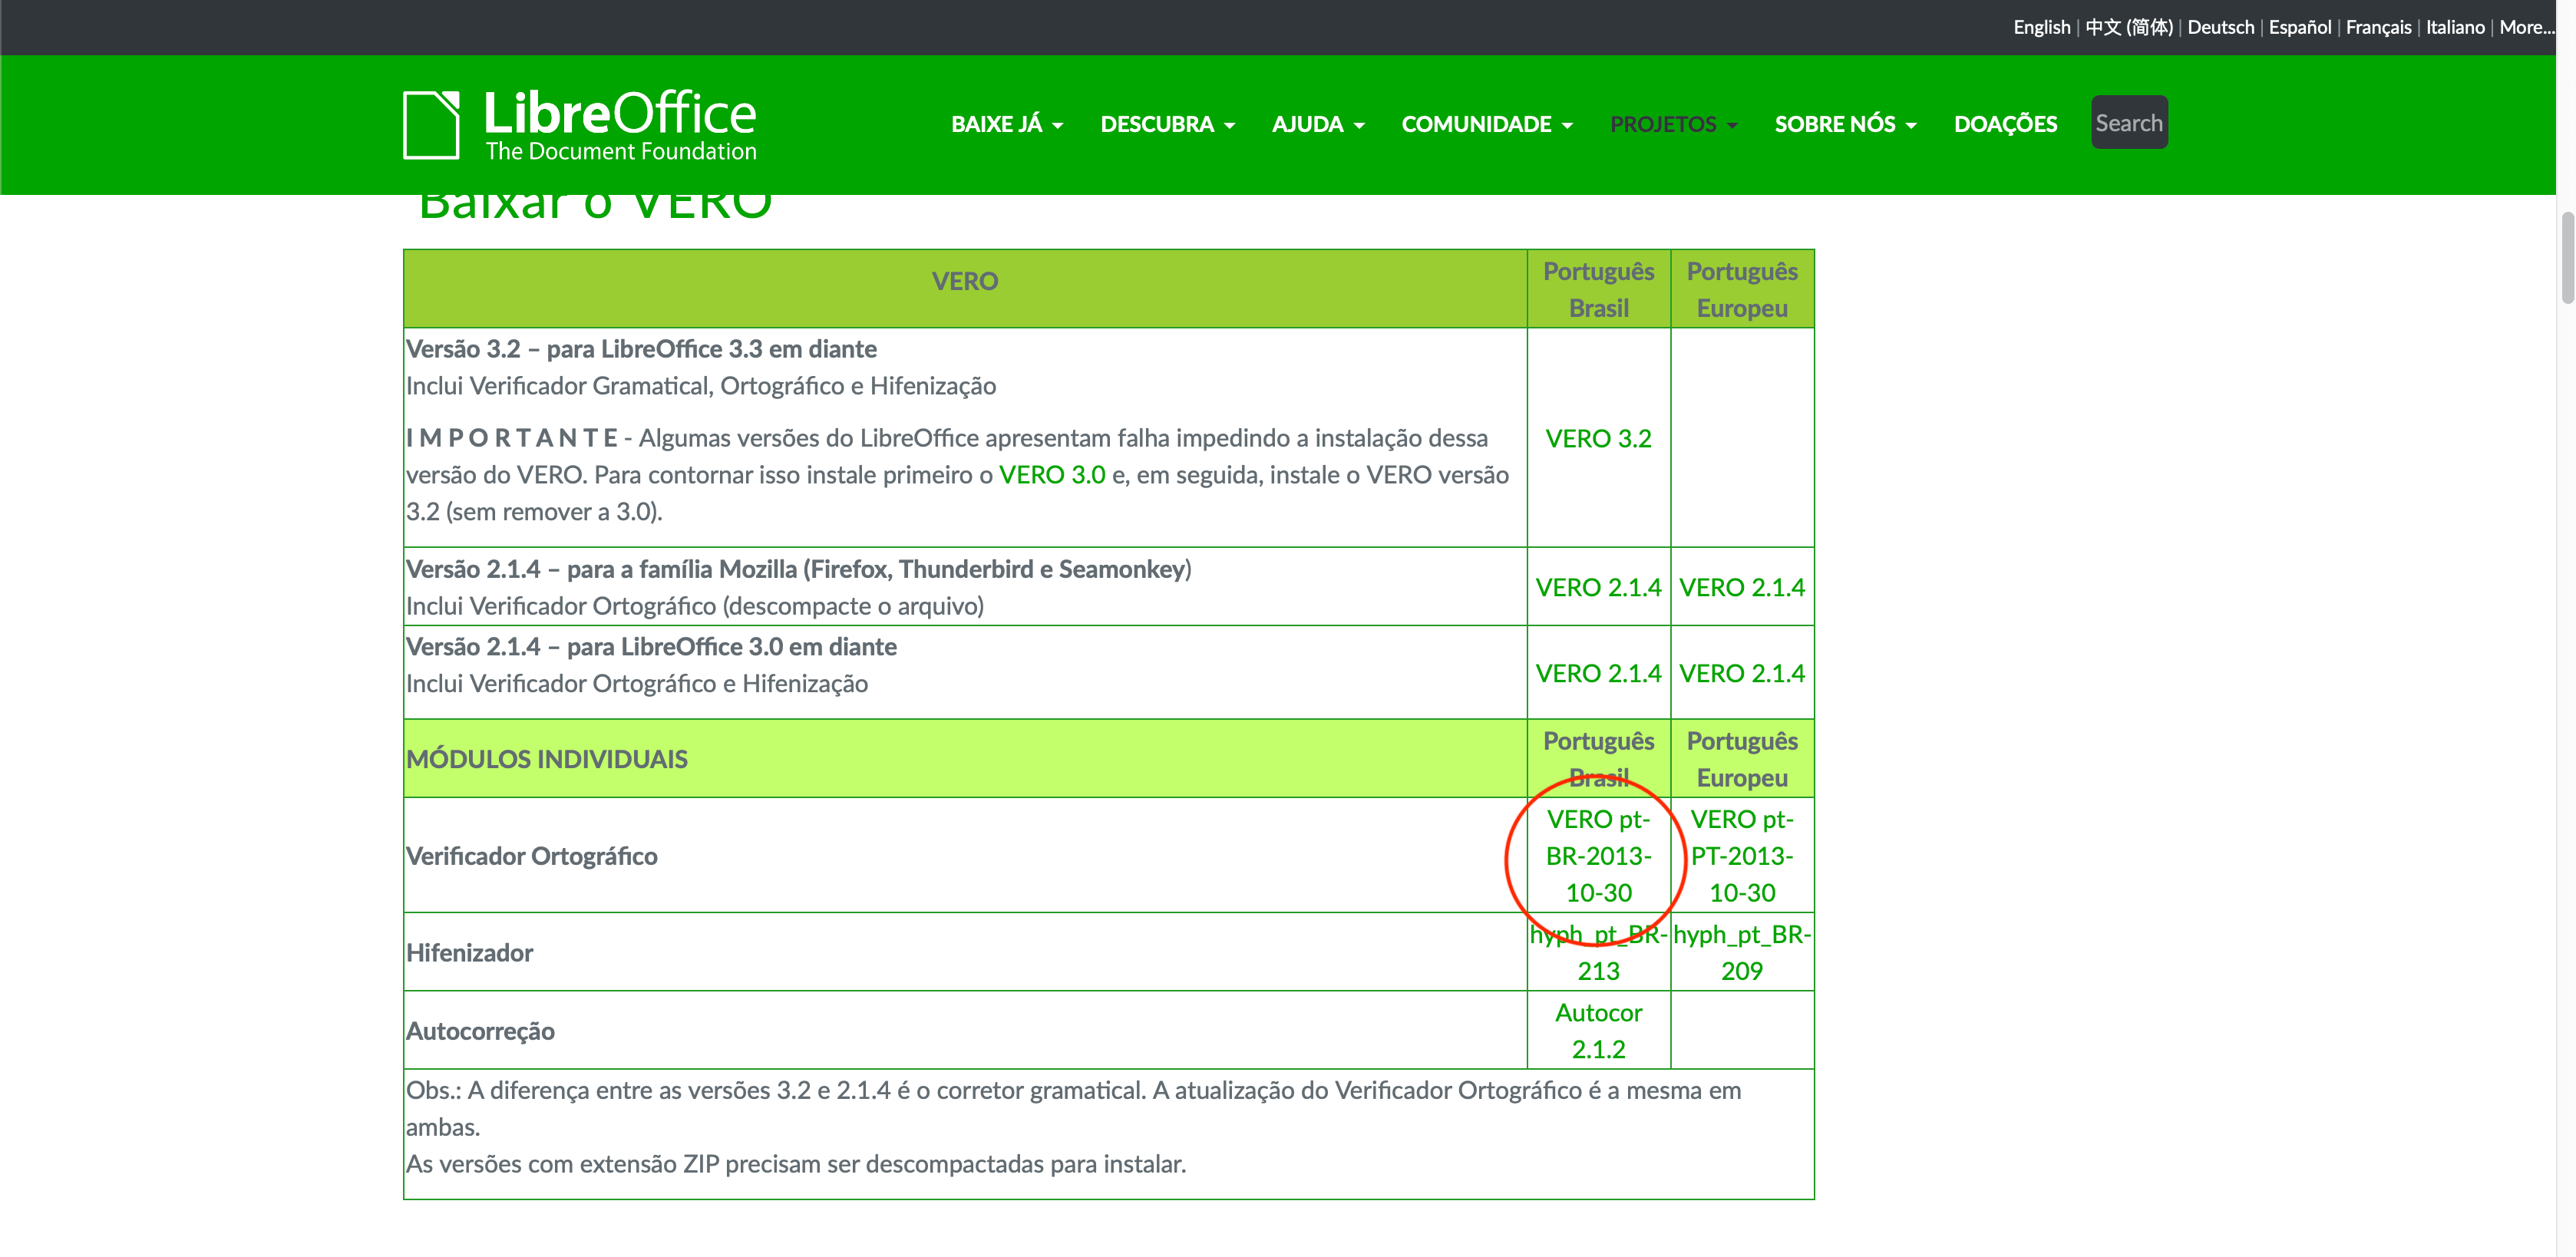
\includegraphics[width=1.0\textwidth]{./fig/vero01}
  \caption{Página de download do corretor ortográfico.}
  \fontefig{Elaborado pelo autor}
\end{figure}
\item Na pasta do arquivo descompactado anteriormente localize os arquivos \aspas{pt\_BR.aff} e \aspas{pt\_BR.dic} e copie eles.
\begin{figure}[H]
  \centering
  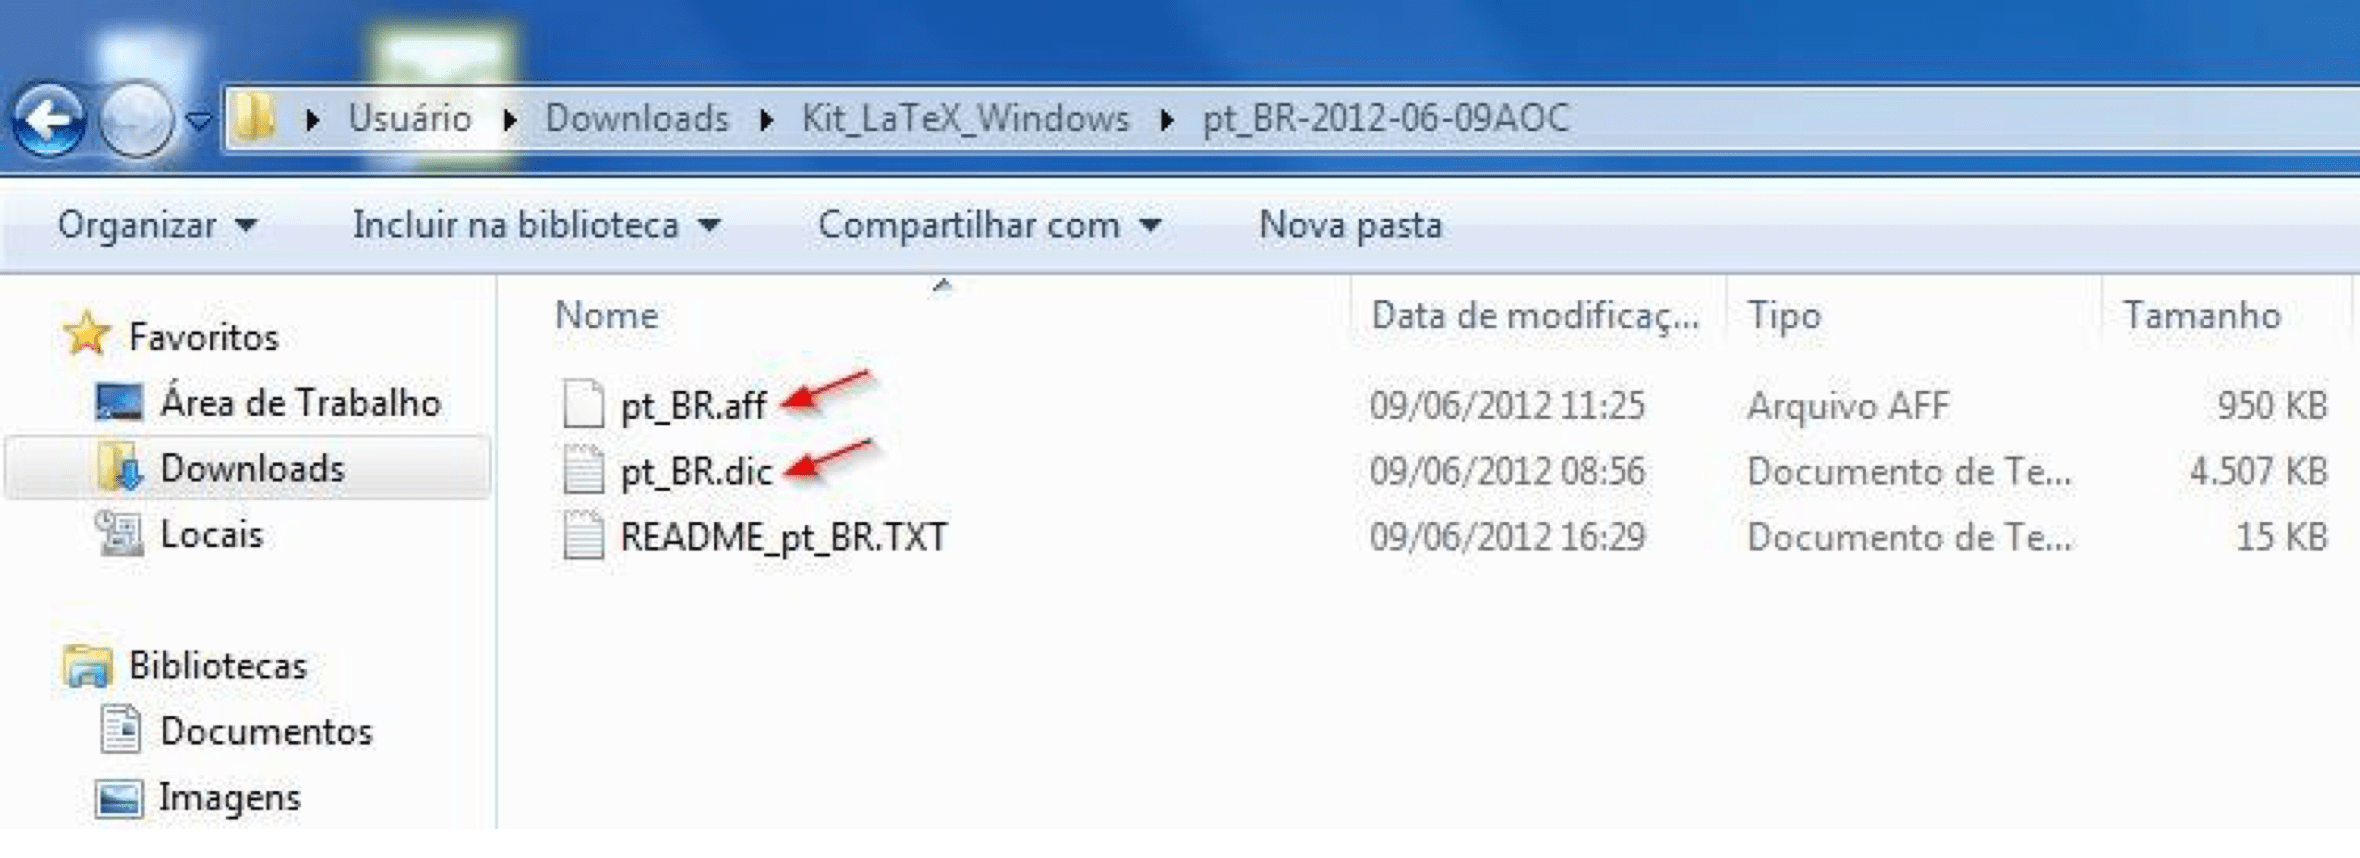
\includegraphics[width=1.0\textwidth]{./fig/vero02}
  \caption{Instalação do corretor ortográfico - Primeira tela.}
  \fontefig{\cite{texnic}}
\end{figure}
\item Localize a pasta de instalação do TeXnicCenter (neste tutorial é a pasta: \aspas{C:$\backslash$Program Files (x86)$\backslash$TeXnicCenter}, mas pode variar de acordo com a versão do Windows utilizada) e dentro dela localize a pasta \textbf{Language}.
\begin{figure}[H]
  \centering
  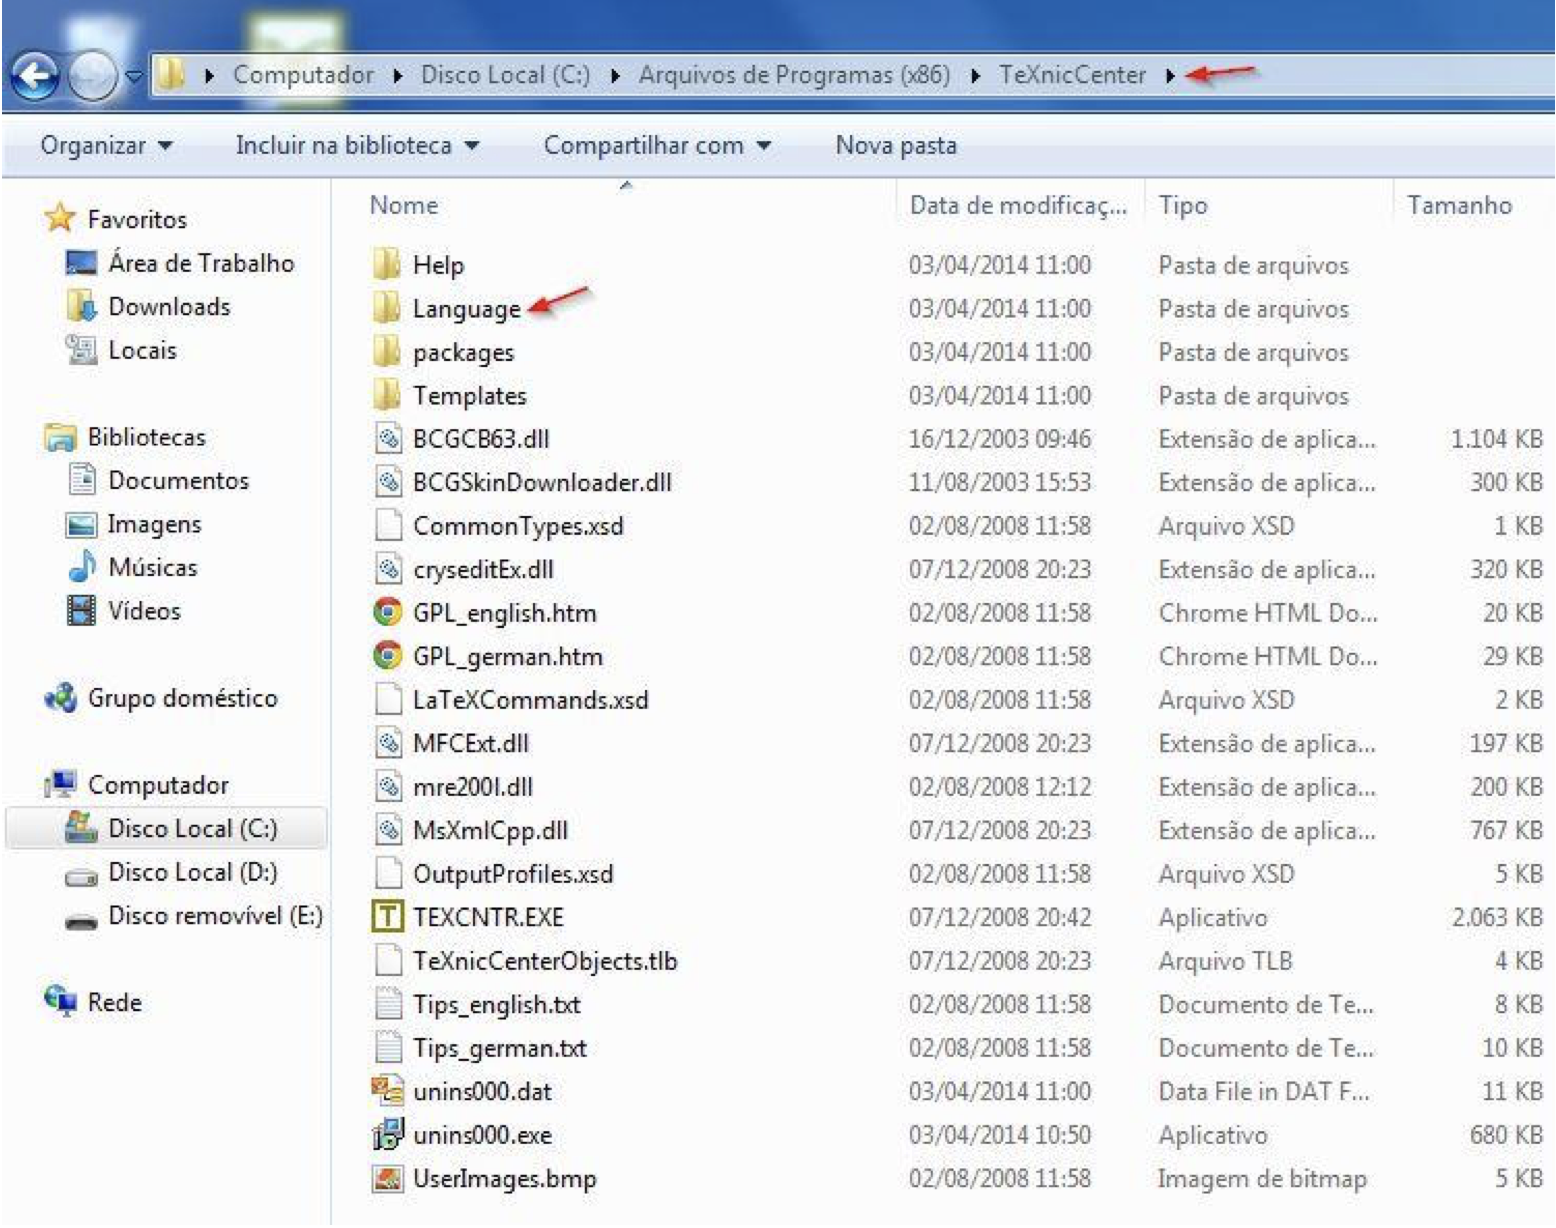
\includegraphics[width=1.0\textwidth]{./fig/vero03}
  \caption{Instalação do corretor ortográfico - Segunda tela.}
  \fontefig{\cite{texnic}}
\end{figure}
\item Cole os arquivos anteriormente copiados dentro da pasta \textbf{Language}.
\begin{figure}[H]
  \centering
  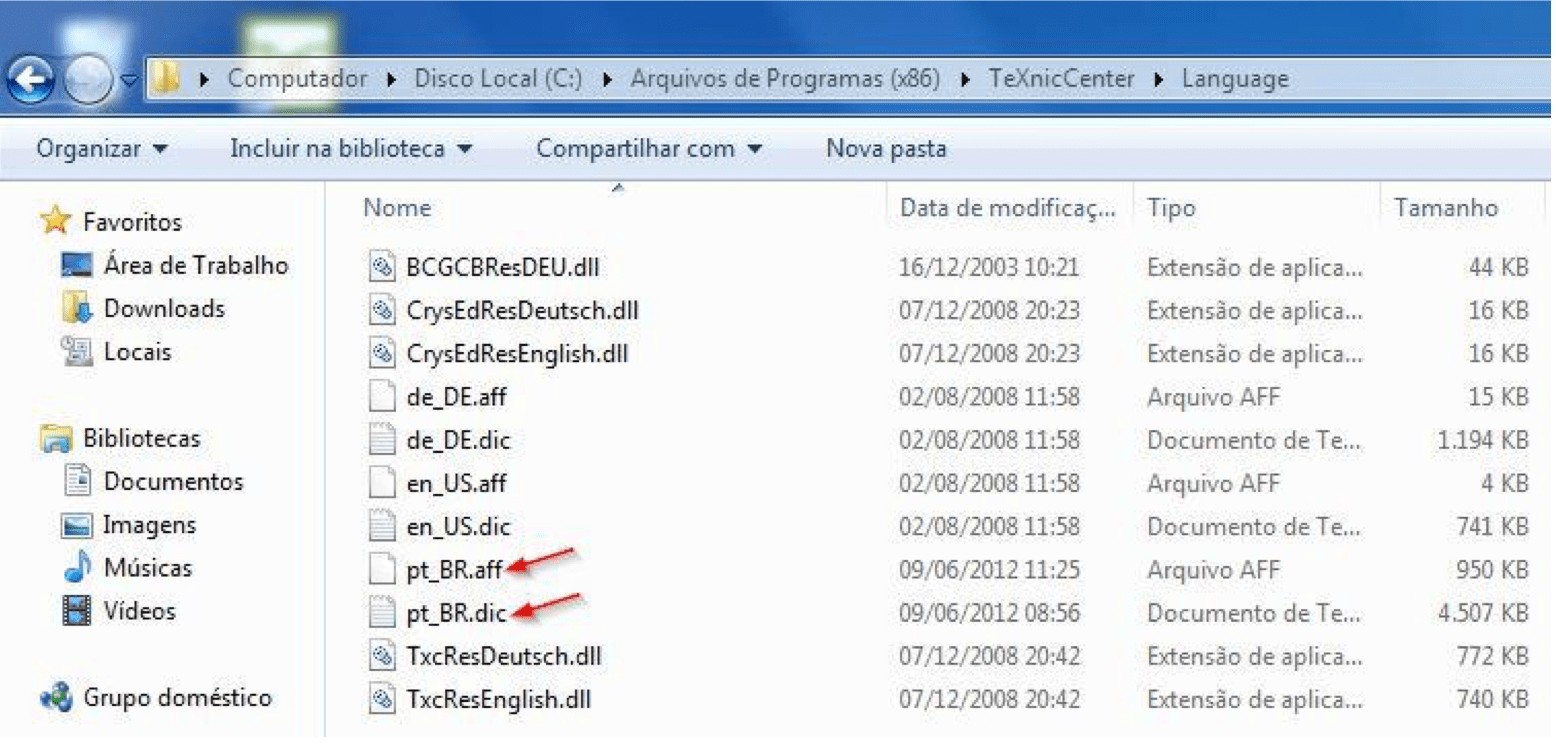
\includegraphics[width=1.0\textwidth]{./fig/vero04}
  \caption{Instalação do corretor ortográfico - Terceira tela.}
  \fontefig{\cite{texnic}}
\end{figure}
\item Para configurar o verificador ortográfico no TeXnicCenter, abra o aplicativo e no menu clique na opção \textbf{Tools}.
\begin{figure}[H]
  \centering
  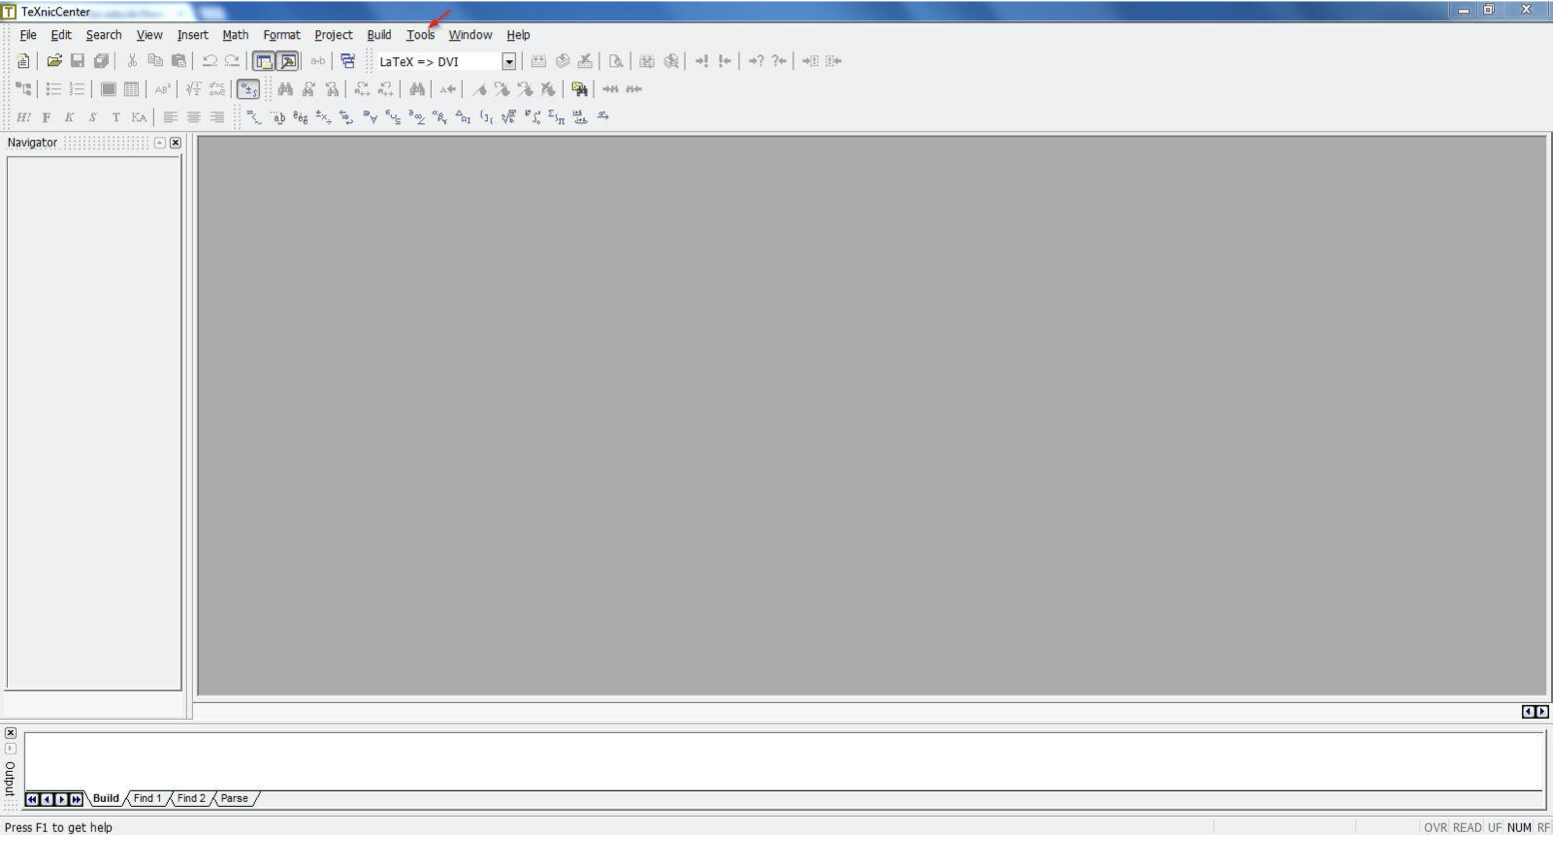
\includegraphics[width=1.0\textwidth]{./fig/vero05}
  \caption{Instalação do corretor ortográfico - Quarta tela.}
  \fontefig{\cite{texnic}}
\end{figure}
\item Agora nas opções abertas do menu é necessário clicar na opção \textbf{Options...}.
\begin{figure}[H]
  \centering
  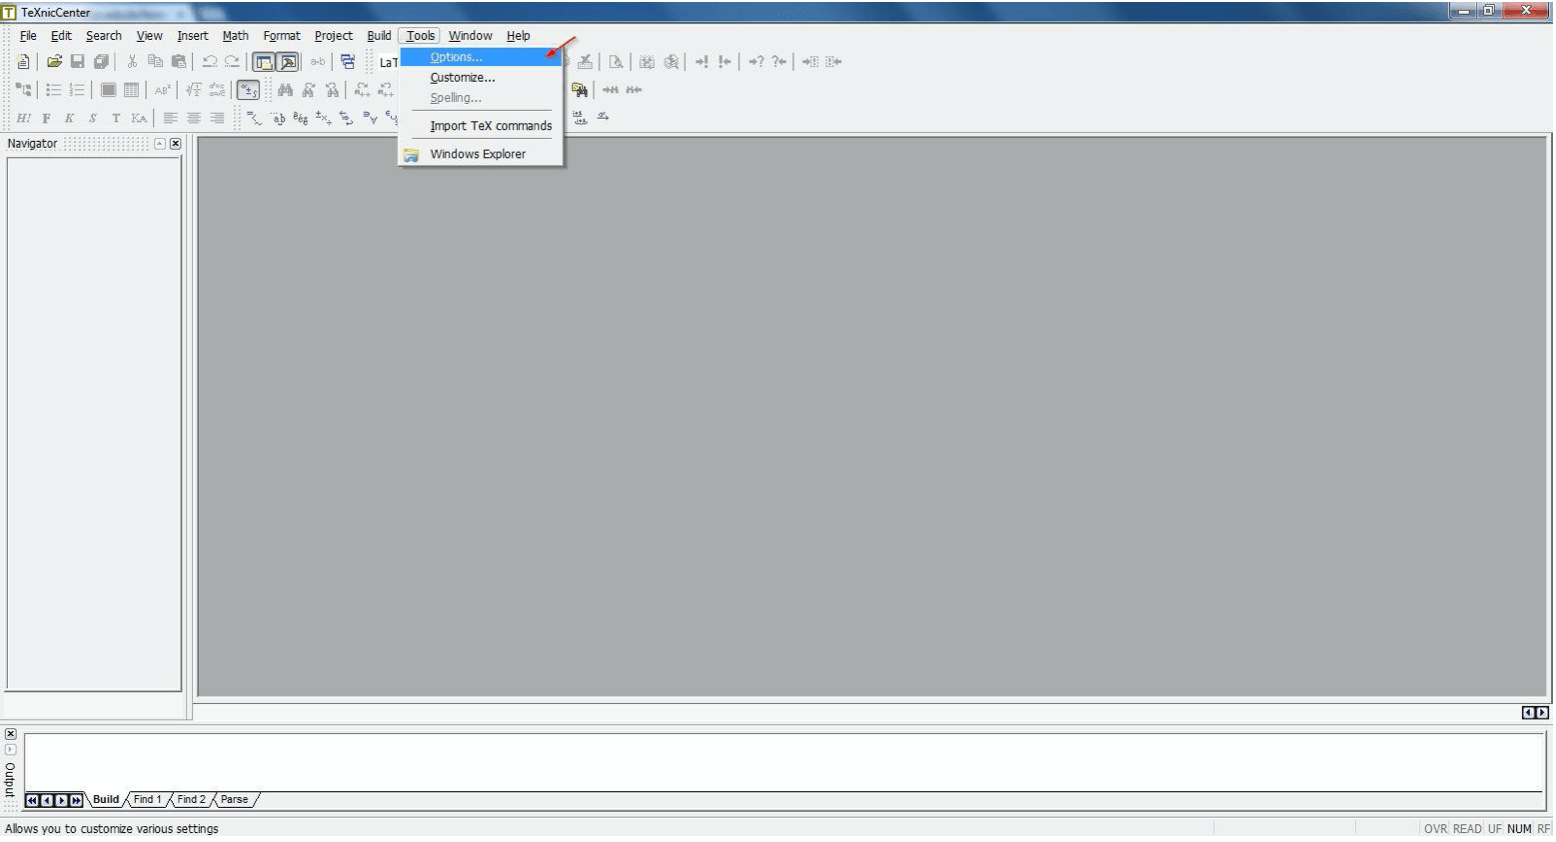
\includegraphics[width=1.0\textwidth]{./fig/vero06}
  \caption{Instalação do corretor ortográfico - Quinta tela.}
  \fontefig{\cite{texnic}}
\end{figure}
\item Na janela de opções aberta clique na aba \textbf{Spelling}.
\begin{figure}[H]
  \centering
  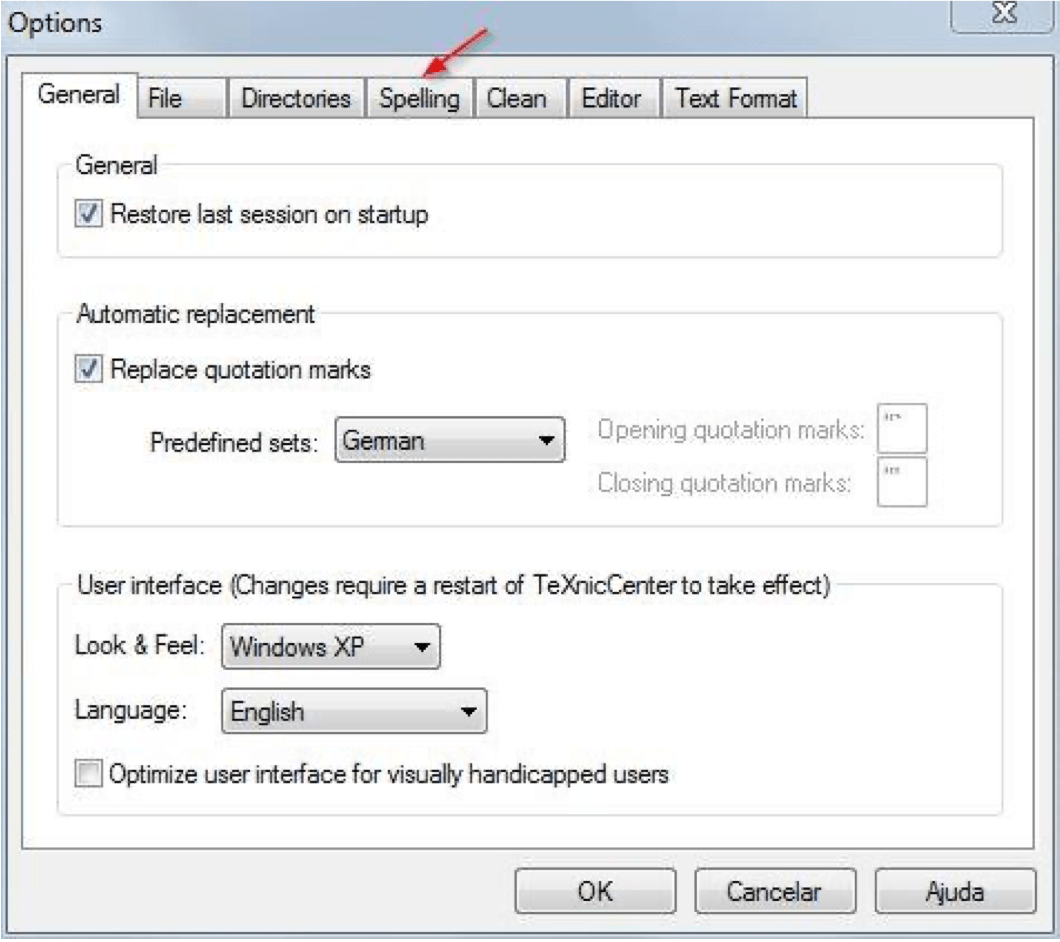
\includegraphics[width=0.6\textwidth]{./fig/vero07}
  \caption{Instalação do corretor ortográfico - Sexta tela.}
  \fontefig{\cite{texnic}}
\end{figure}
\item Na Na aba aberta na opção \textbf{Language} selecione \textbf{pt}, na opção \textbf{Dialect} selecione \textbf{BR}, na opção \textbf{Locale} selecione \textbf{Portuguese\_Brazil.1252} e na seção \textbf{Options} clique na caixa ao lado de \textbf{Check spelling while typing} para setar as opções de correção ortográfica. Após selecionadas as opções clique no botão \textbf{OK}.
\begin{figure}[H]
  \centering
  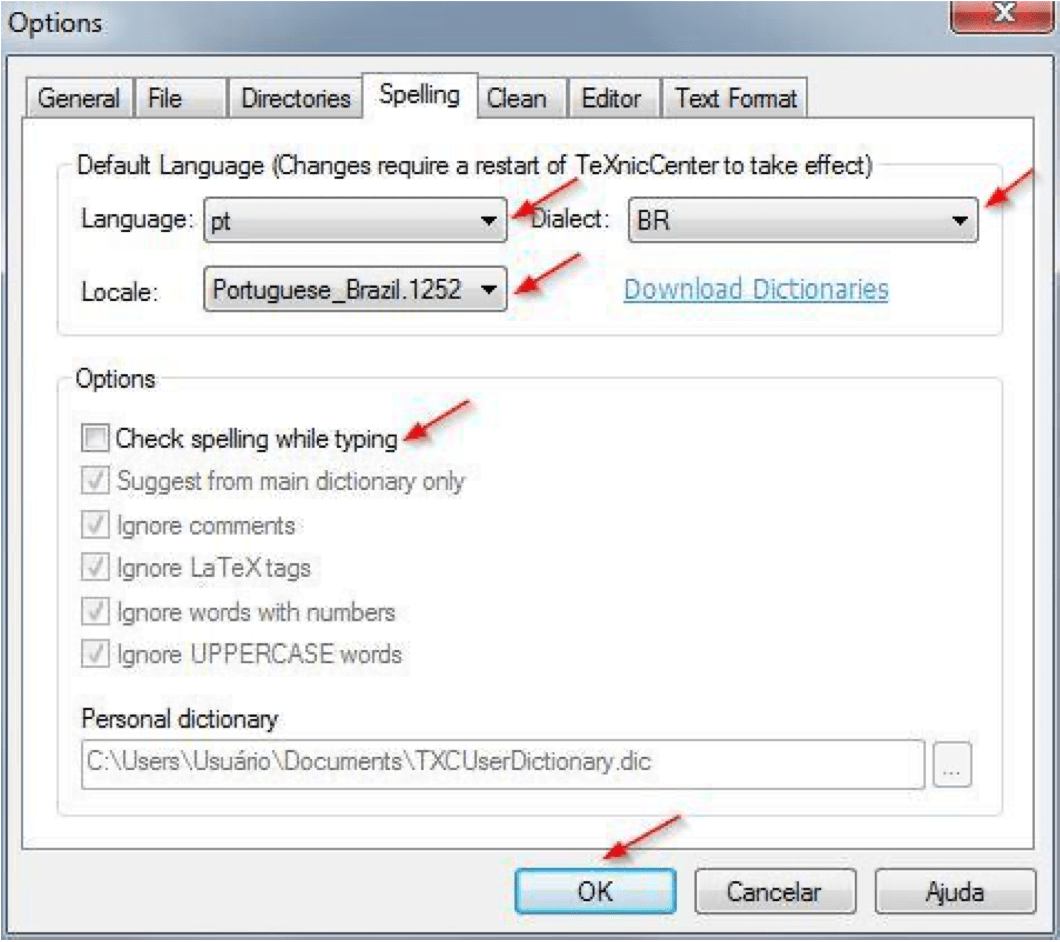
\includegraphics[width=0.6\textwidth]{./fig/vero08}
  \caption{Instalação do corretor ortográfico - Sétima tela.}
  \fontefig{\cite{texnic}}
\end{figure}
\item A caixa de diálogo abaixo será exibida informando que é necessário reiniciar o TeXnicCenter para que as opções selecionadas anteriormente tenham efeito. Clique no botão \textbf{OK} para fechar.
\begin{figure}[H]
  \centering
  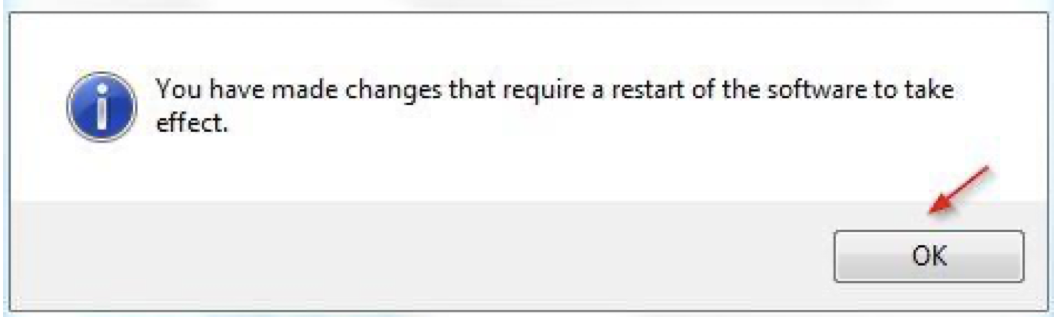
\includegraphics[width=0.6\textwidth]{./fig/vero09}
  \caption{Instalação do corretor ortográfico - Oitava tela.}
  \fontefig{\cite{texnic}}
\end{figure}
\item Será exibida uma caixa de diálogo informando que o dicionário de usuário não foi encontrado e que foi criado um novo dicionário pessoal vazio. Clique no botão \textbf{OK} para fechar.
\begin{figure}[H]
  \centering
  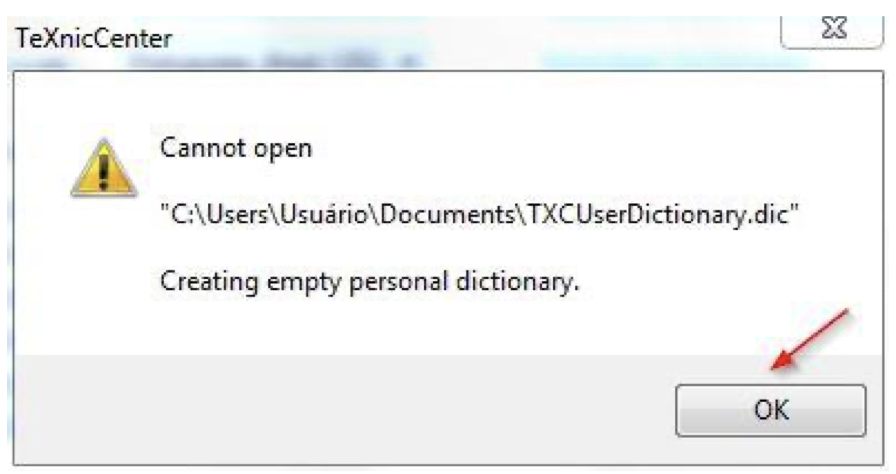
\includegraphics[width=0.5\textwidth]{./fig/vero10}
  \caption{Instalação do corretor ortográfico - Nona tela.}
  \fontefig{\cite{texnic}}
\end{figure}
\end{enumerate}

\section{Usando o \LaTeX\ online}

Em vez de utilizar o \LaTeX\ localmente em seu computador você pode utilizá-lo online usando o Overleaf, uma plataforma de escrita colaborativa, cujo objetivo principal  é facilitar o o processo de escrita acadêmica.

Inicialmente crie uma conta em \url{https://www.overleaf.com}. Depois, acesse o endereço \url{https://overleaf.com/docs?snip_uri=https://github.com/raphaeldeaquino/classe-ifg/archive/main.zip} que o projeto será criado automaticamente.